\documentclass[fleqn,10pt]{wlscirep}
\usepackage[utf8]{inputenc}
\usepackage[T1]{fontenc}
\usepackage{makecell}

\title{Supplementary Information}

\author[1,2,*,\textsuperscript{\textdagger}]{Carmen Cabrera}
\author[1]{Miguel González-Leonardo}
\author[1,3]{Andrea Nasuto}
\author[2]{Ruth Neville}
\author[1,\textsuperscript{\textdagger}]{Francisco Rowe}
\affil[1]{Geographic Data Science Lab, Department of Geography and Planning, University of Liverpool, Liverpool, UK}
\affil[2]{Centre for Advanced Spatial Analysis, University College London, London, UK}
\affil[3]{Institute for Quantitative Social Science, Harvard University, Cambridge, US}


\affil[*]{Corresponding author: c.cabrera@liverpool.ac.uk}

\affil[ \textsuperscript{\textdagger}]{These authors have contributed equally to this study.}


%\keywords{Keyword1, Keyword2, Keyword3}


\begin{abstract}
This is the Supplementary Information for the article titled ``Sustained changes to urban mobility after COVID-19 amplified socio-economic inequalities in Latin America''.
\end{abstract}

\begin{document}

\flushbottom

\maketitle
% * <john.hammersley@gmail.com> 2015-02-09T12:07:31.197Z:
%
%  Click the title above to edit the author information and abstract
%

% * <john.hammersley@gmail.com> 2015-02-09T12:07:31.197Z:
%
%  Click the title above to edit the author information and abstract
\vspace{-10mm}
\section{Processing Facebook data}

\subsection{Missing values}

\begin{table}[h!]
\centering
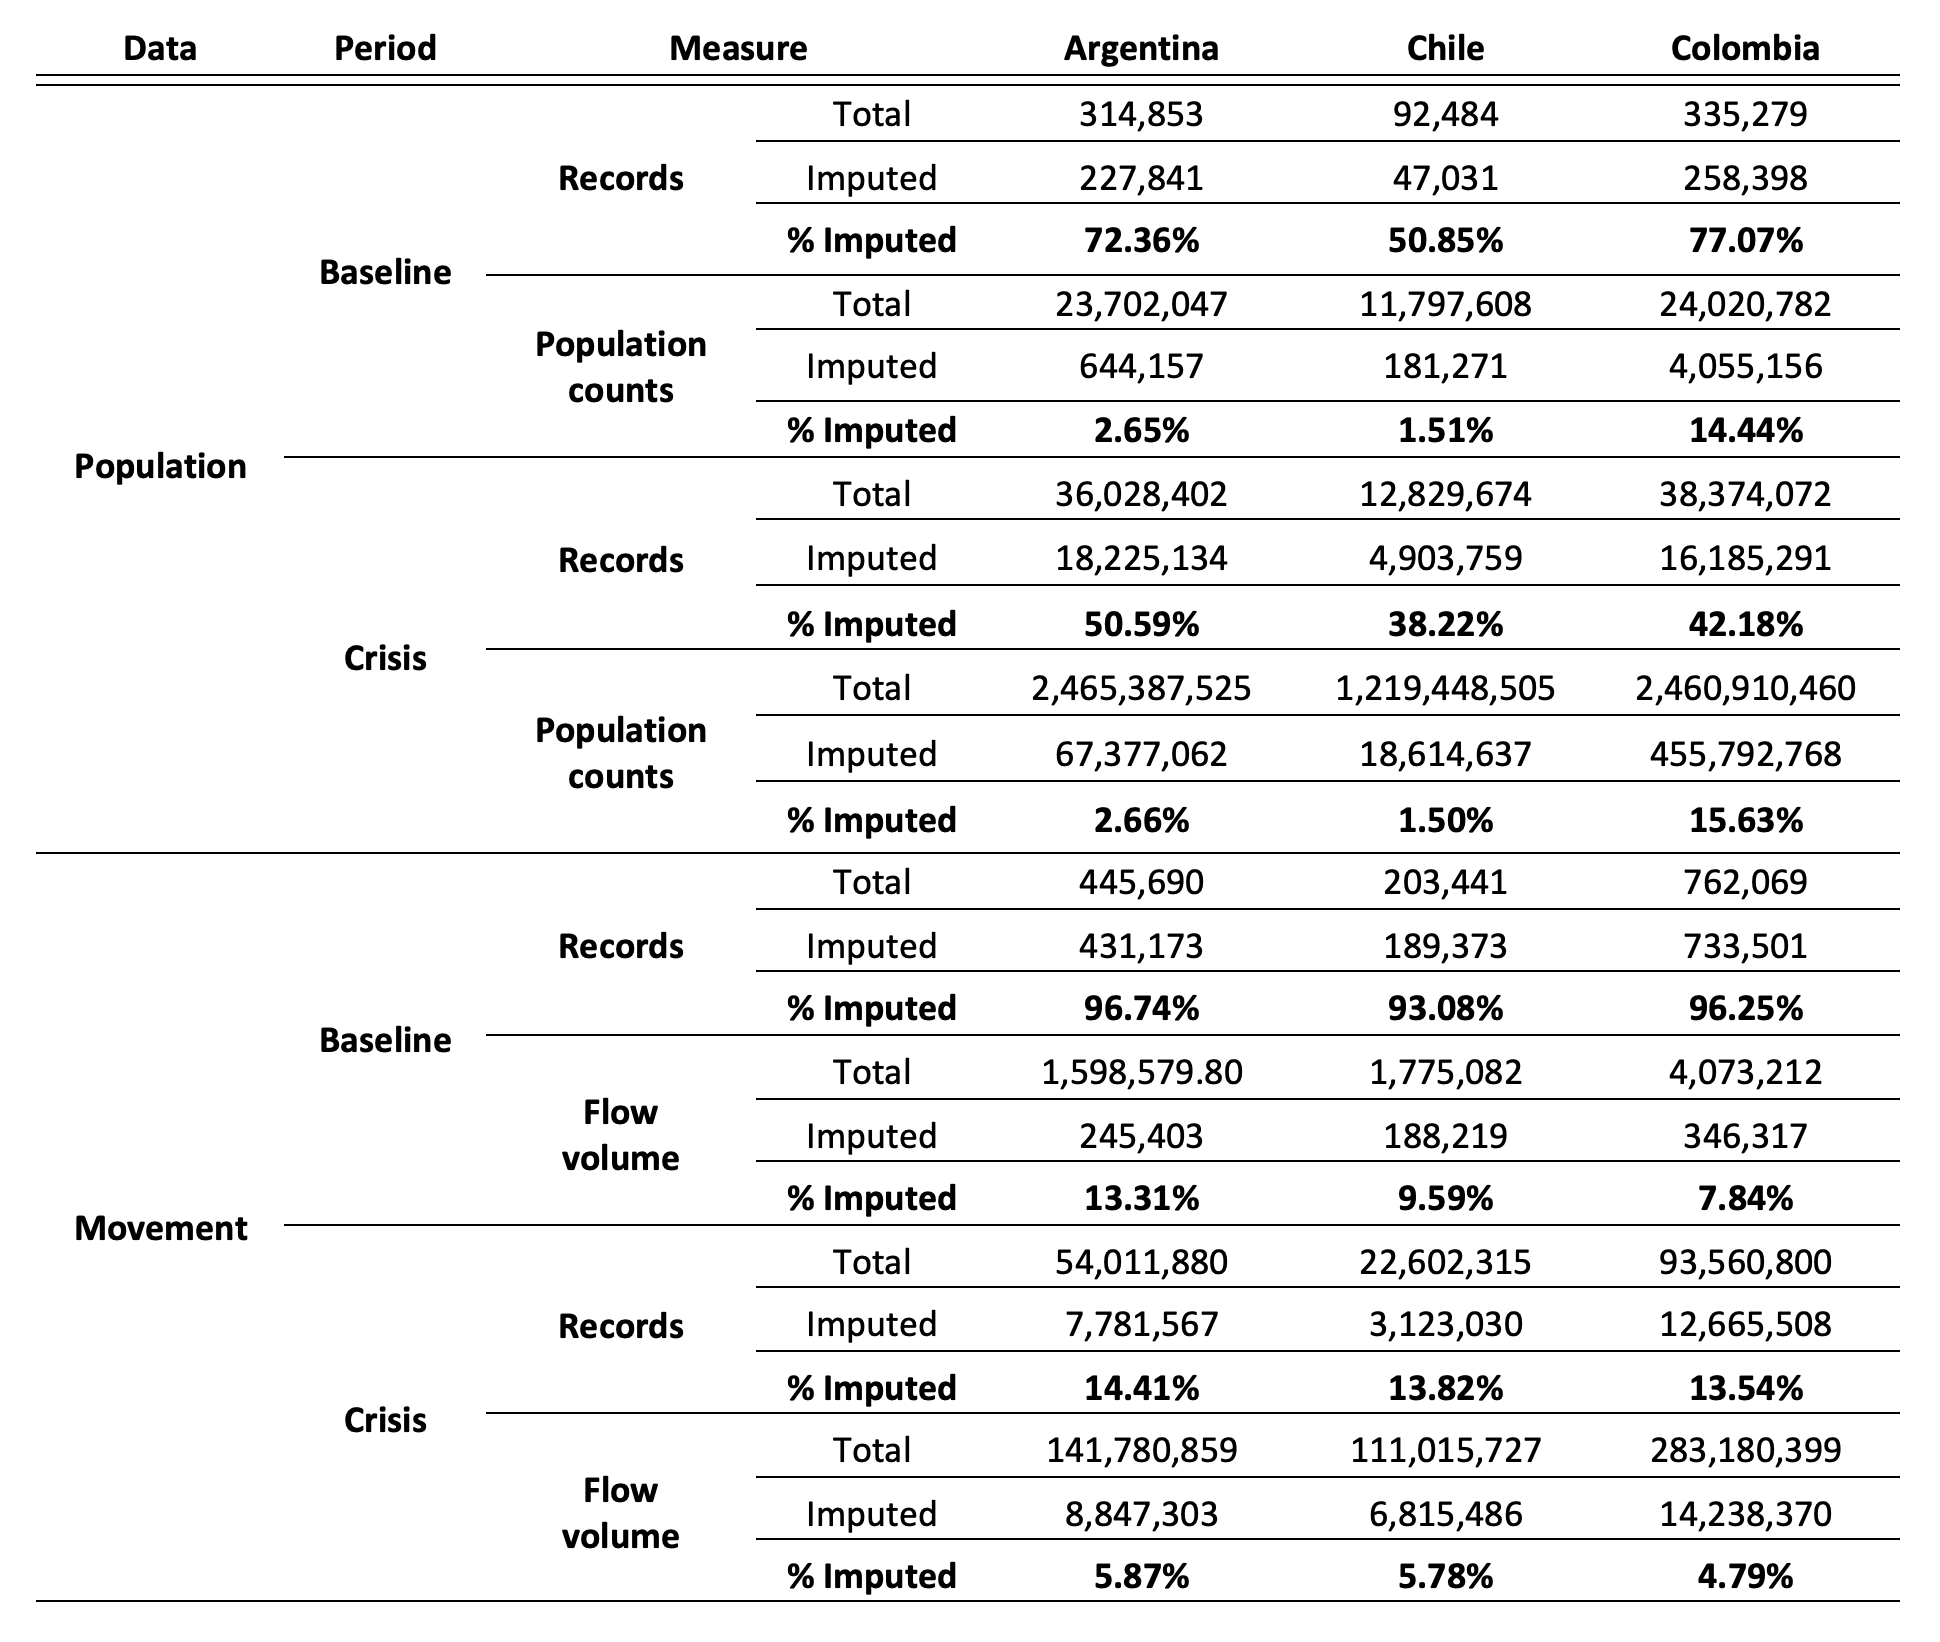
\includegraphics[width=0.8\linewidth]{supplementary/missing/SF-missing-data-table-r2.png}
\caption{Summary of imputation in the Facebook Population and Facebook Movement datasets during the baseline and crisis periods for Argentina, Chile and Colombia. The table reports, for each dataset and period, total records, imputed records and the percentage of records imputed, as well as total population or flows, imputed population or flows and the percentage of the final total contributed by imputation.}
\end{table}

\newpage

\begin{figure}[h!]
\centering
\includegraphics[width=.7\linewidth]{supplementary/missing/SF-missing.png}
\caption{Facebook Population baseline records corresponding to Monday, for Argentina, Chile and Colombia. The first row shows the original records, which include a high proportion of missing values. The second row shows the imputed baseline following a regression model with Worldpop data. This figure provides descriptive insight into the baseline population measure used in the analysis.}
\label{missing-baseline}
\end{figure}

\newpage

\subsection{Relationship between WorldPop population and Facebook Population baseline data for each day of the week}

\begin{figure}[h!]
\centering
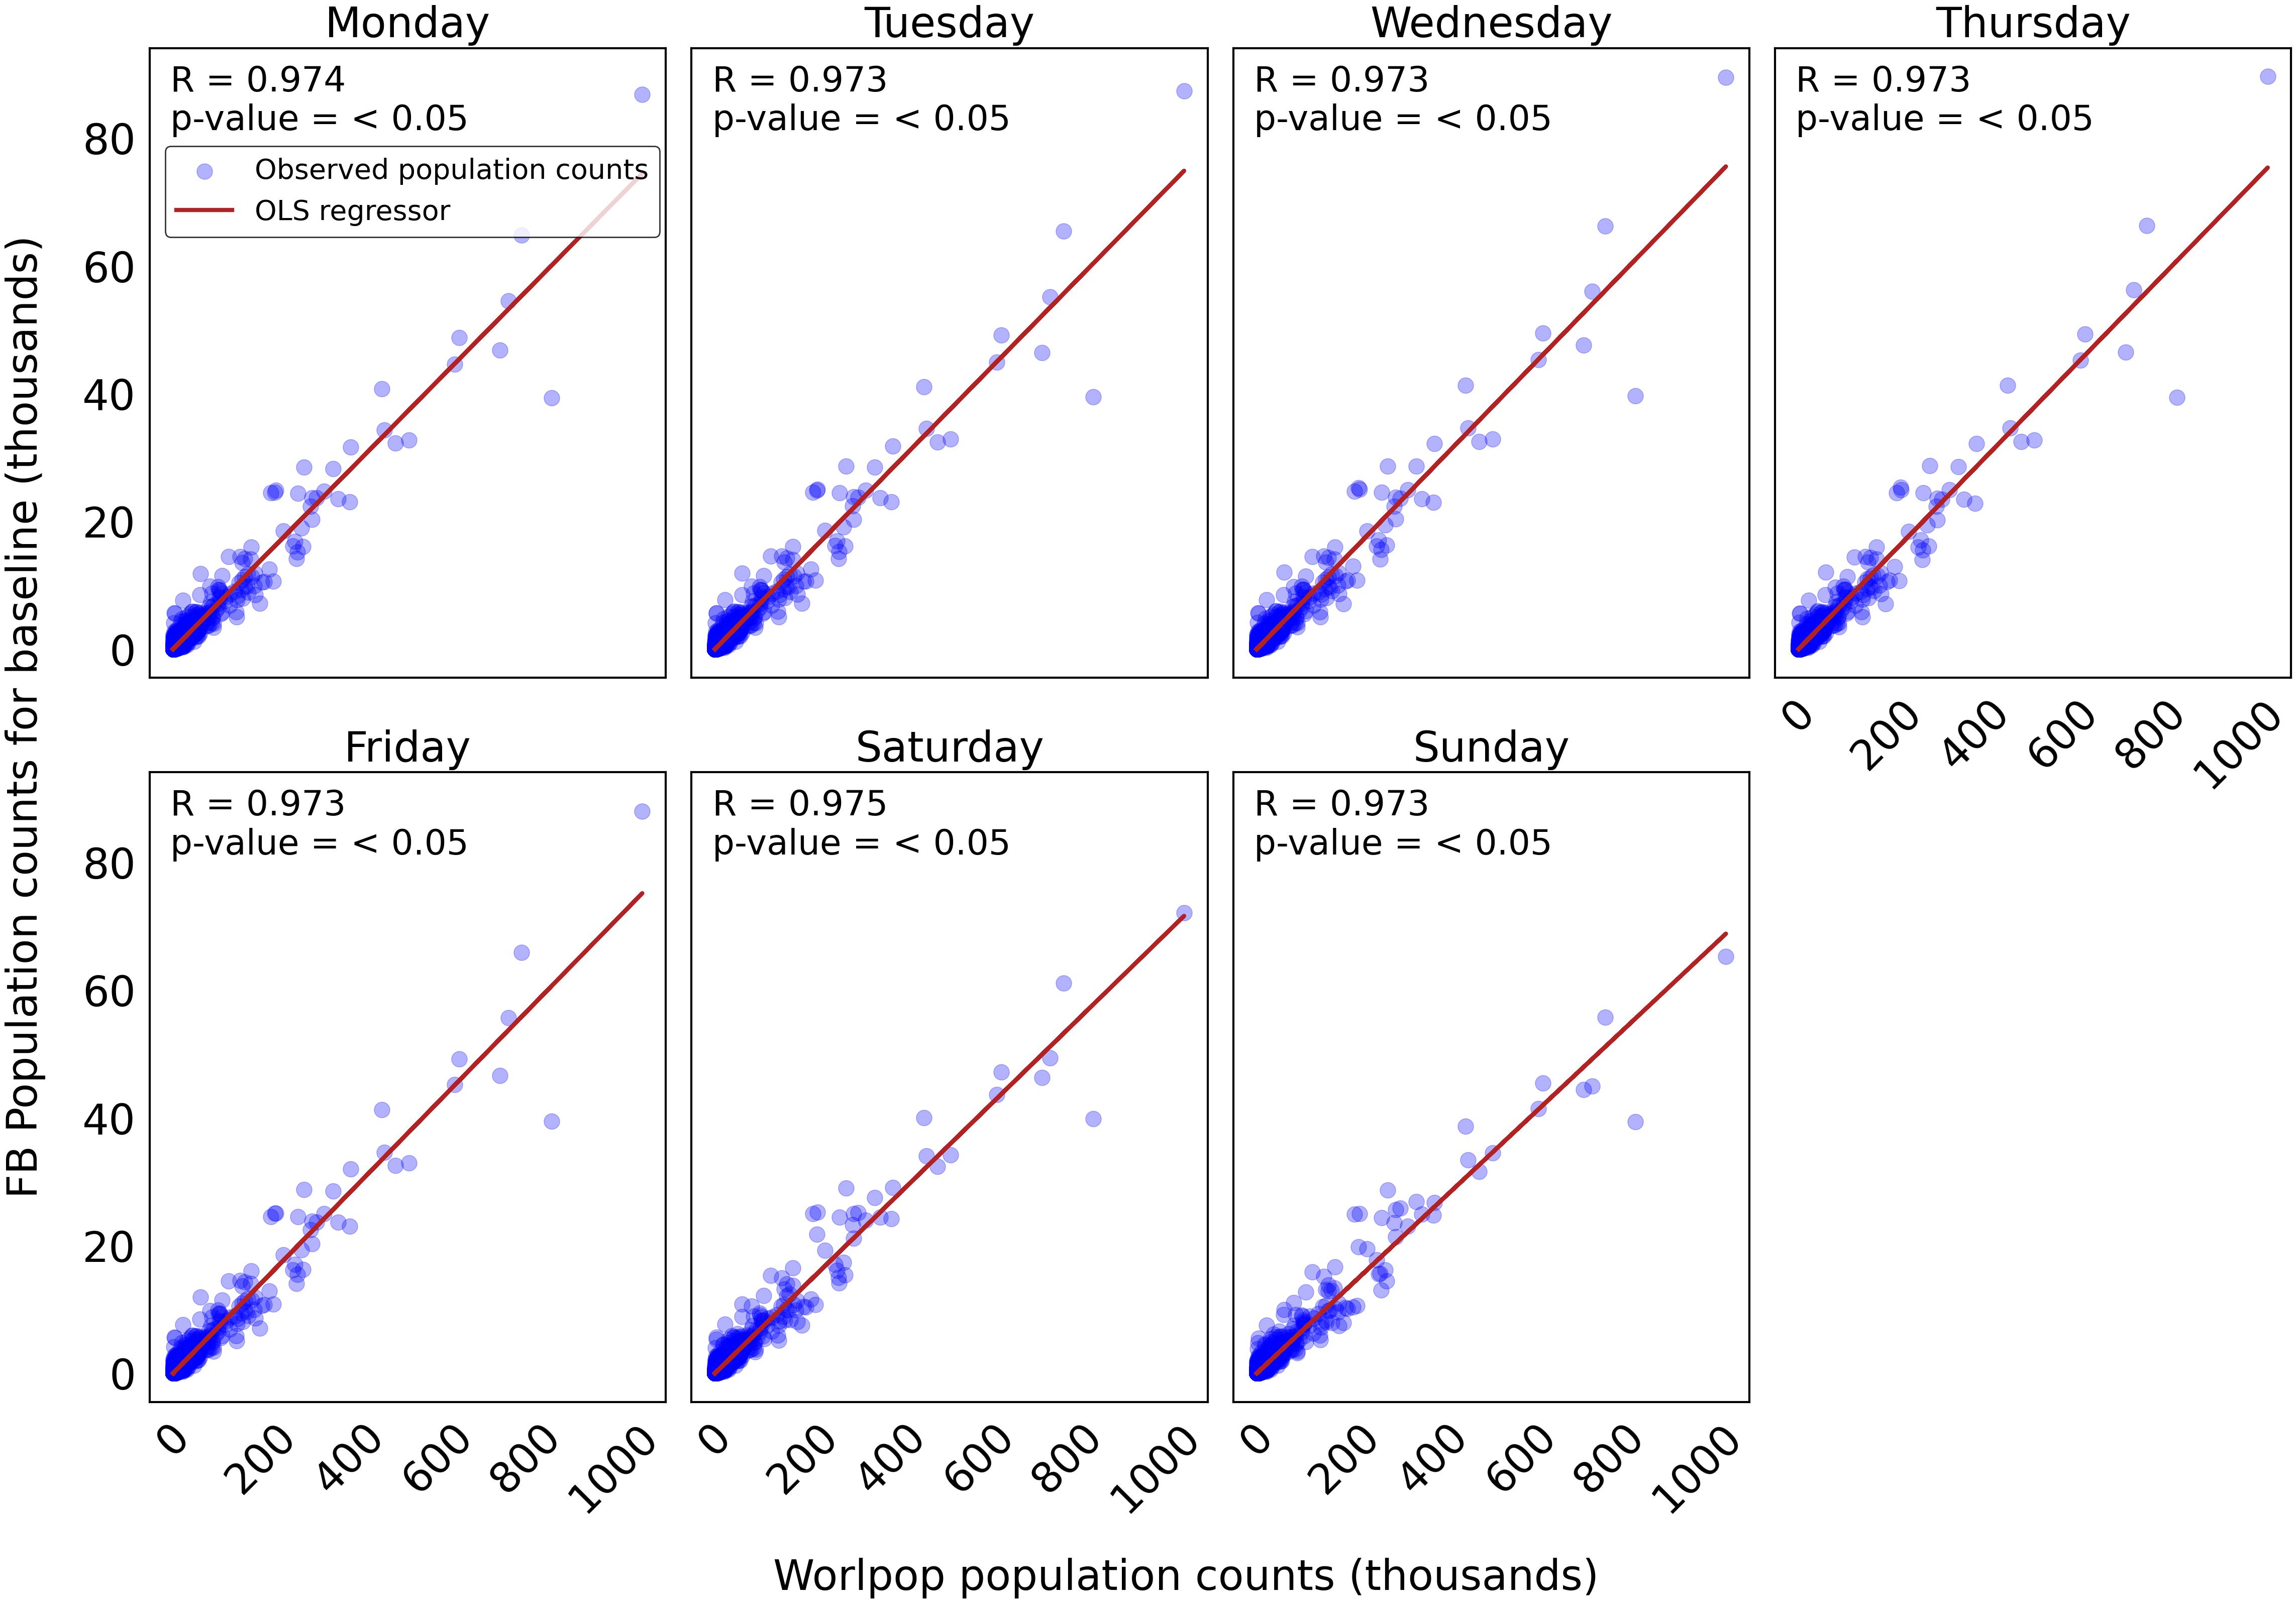
\includegraphics[width=\linewidth]{supplementary/correlation/correlation-wp-fb-pop-baseline-ARG.png}
\caption{Correlation between Worldpop population counts and Facebook Population counts during the baseline period in Argentina, for each day of the week.}
\label{correlation-wp-fbpop-ARG}
\end{figure}

\newpage

\begin{figure}[h!]
\centering
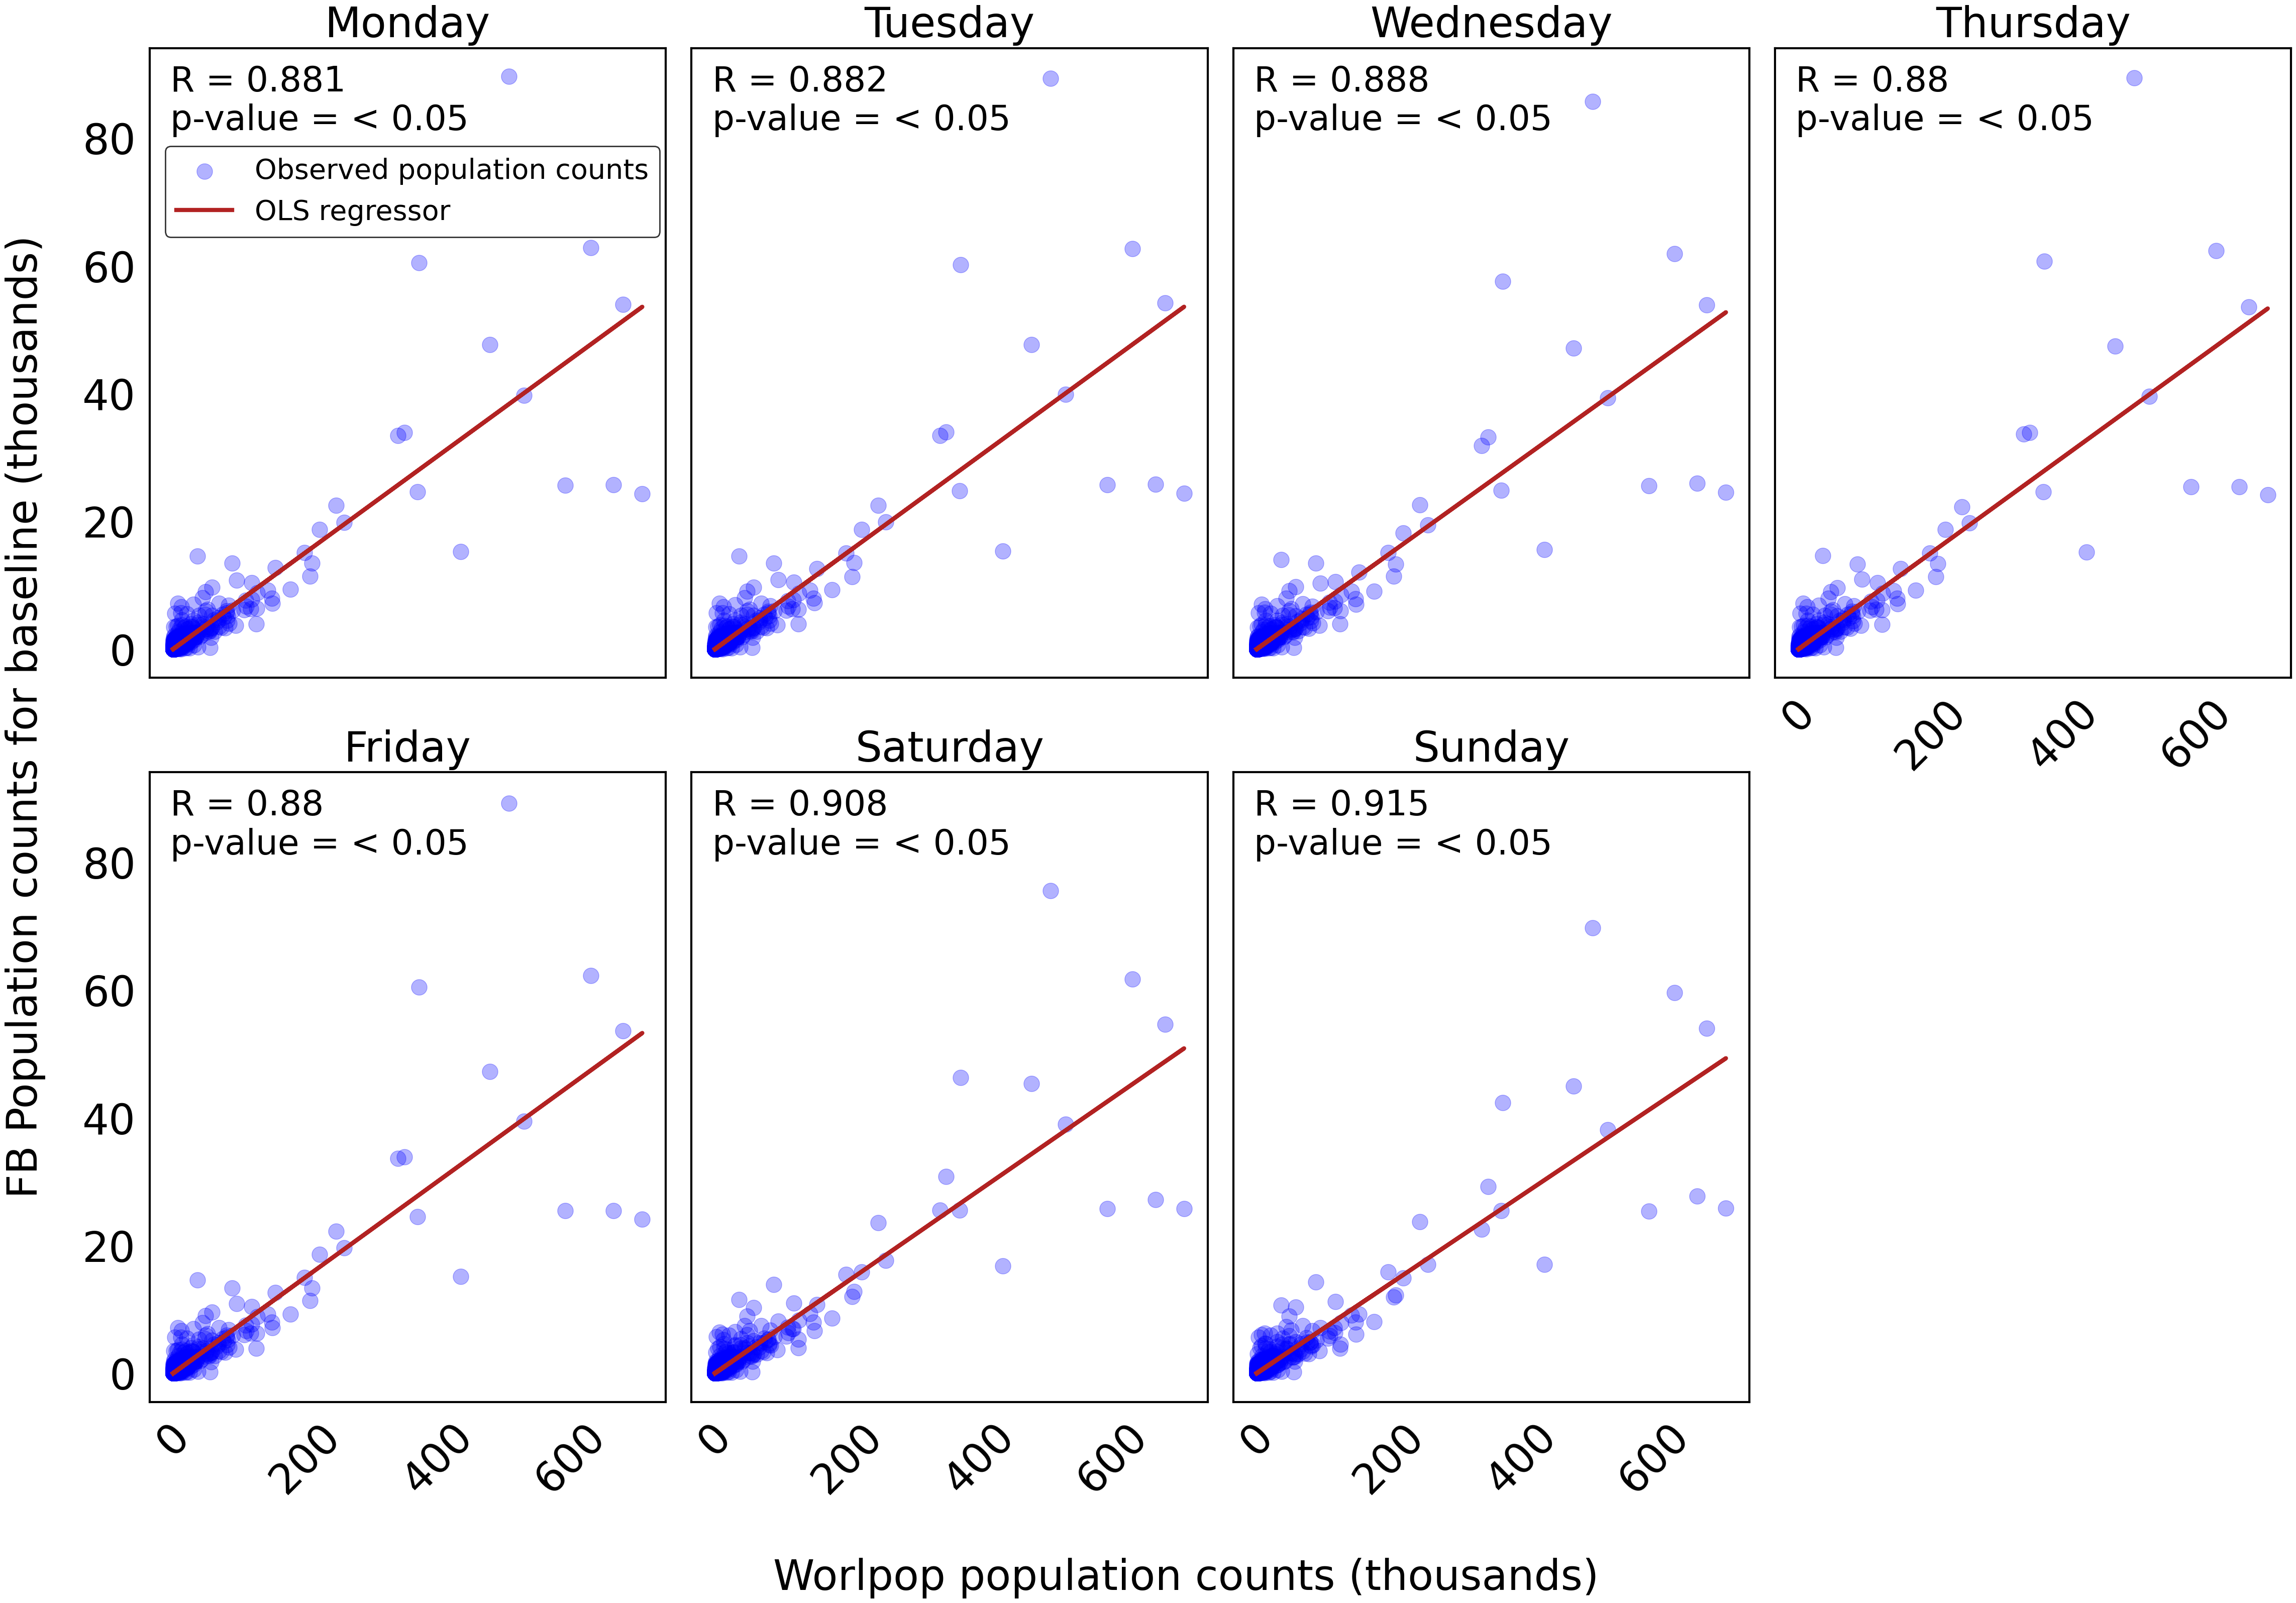
\includegraphics[width=\linewidth]{supplementary/correlation/correlation-wp-fb-pop-baseline-CHL.png}
\caption{Correlation between Worldpop population counts and Facebook Population counts during the baseline period in Chile, for each day of the week.}
\label{correlation-wp-fbpop-CHL}
\end{figure}

\newpage

\begin{figure}[h!]
\centering
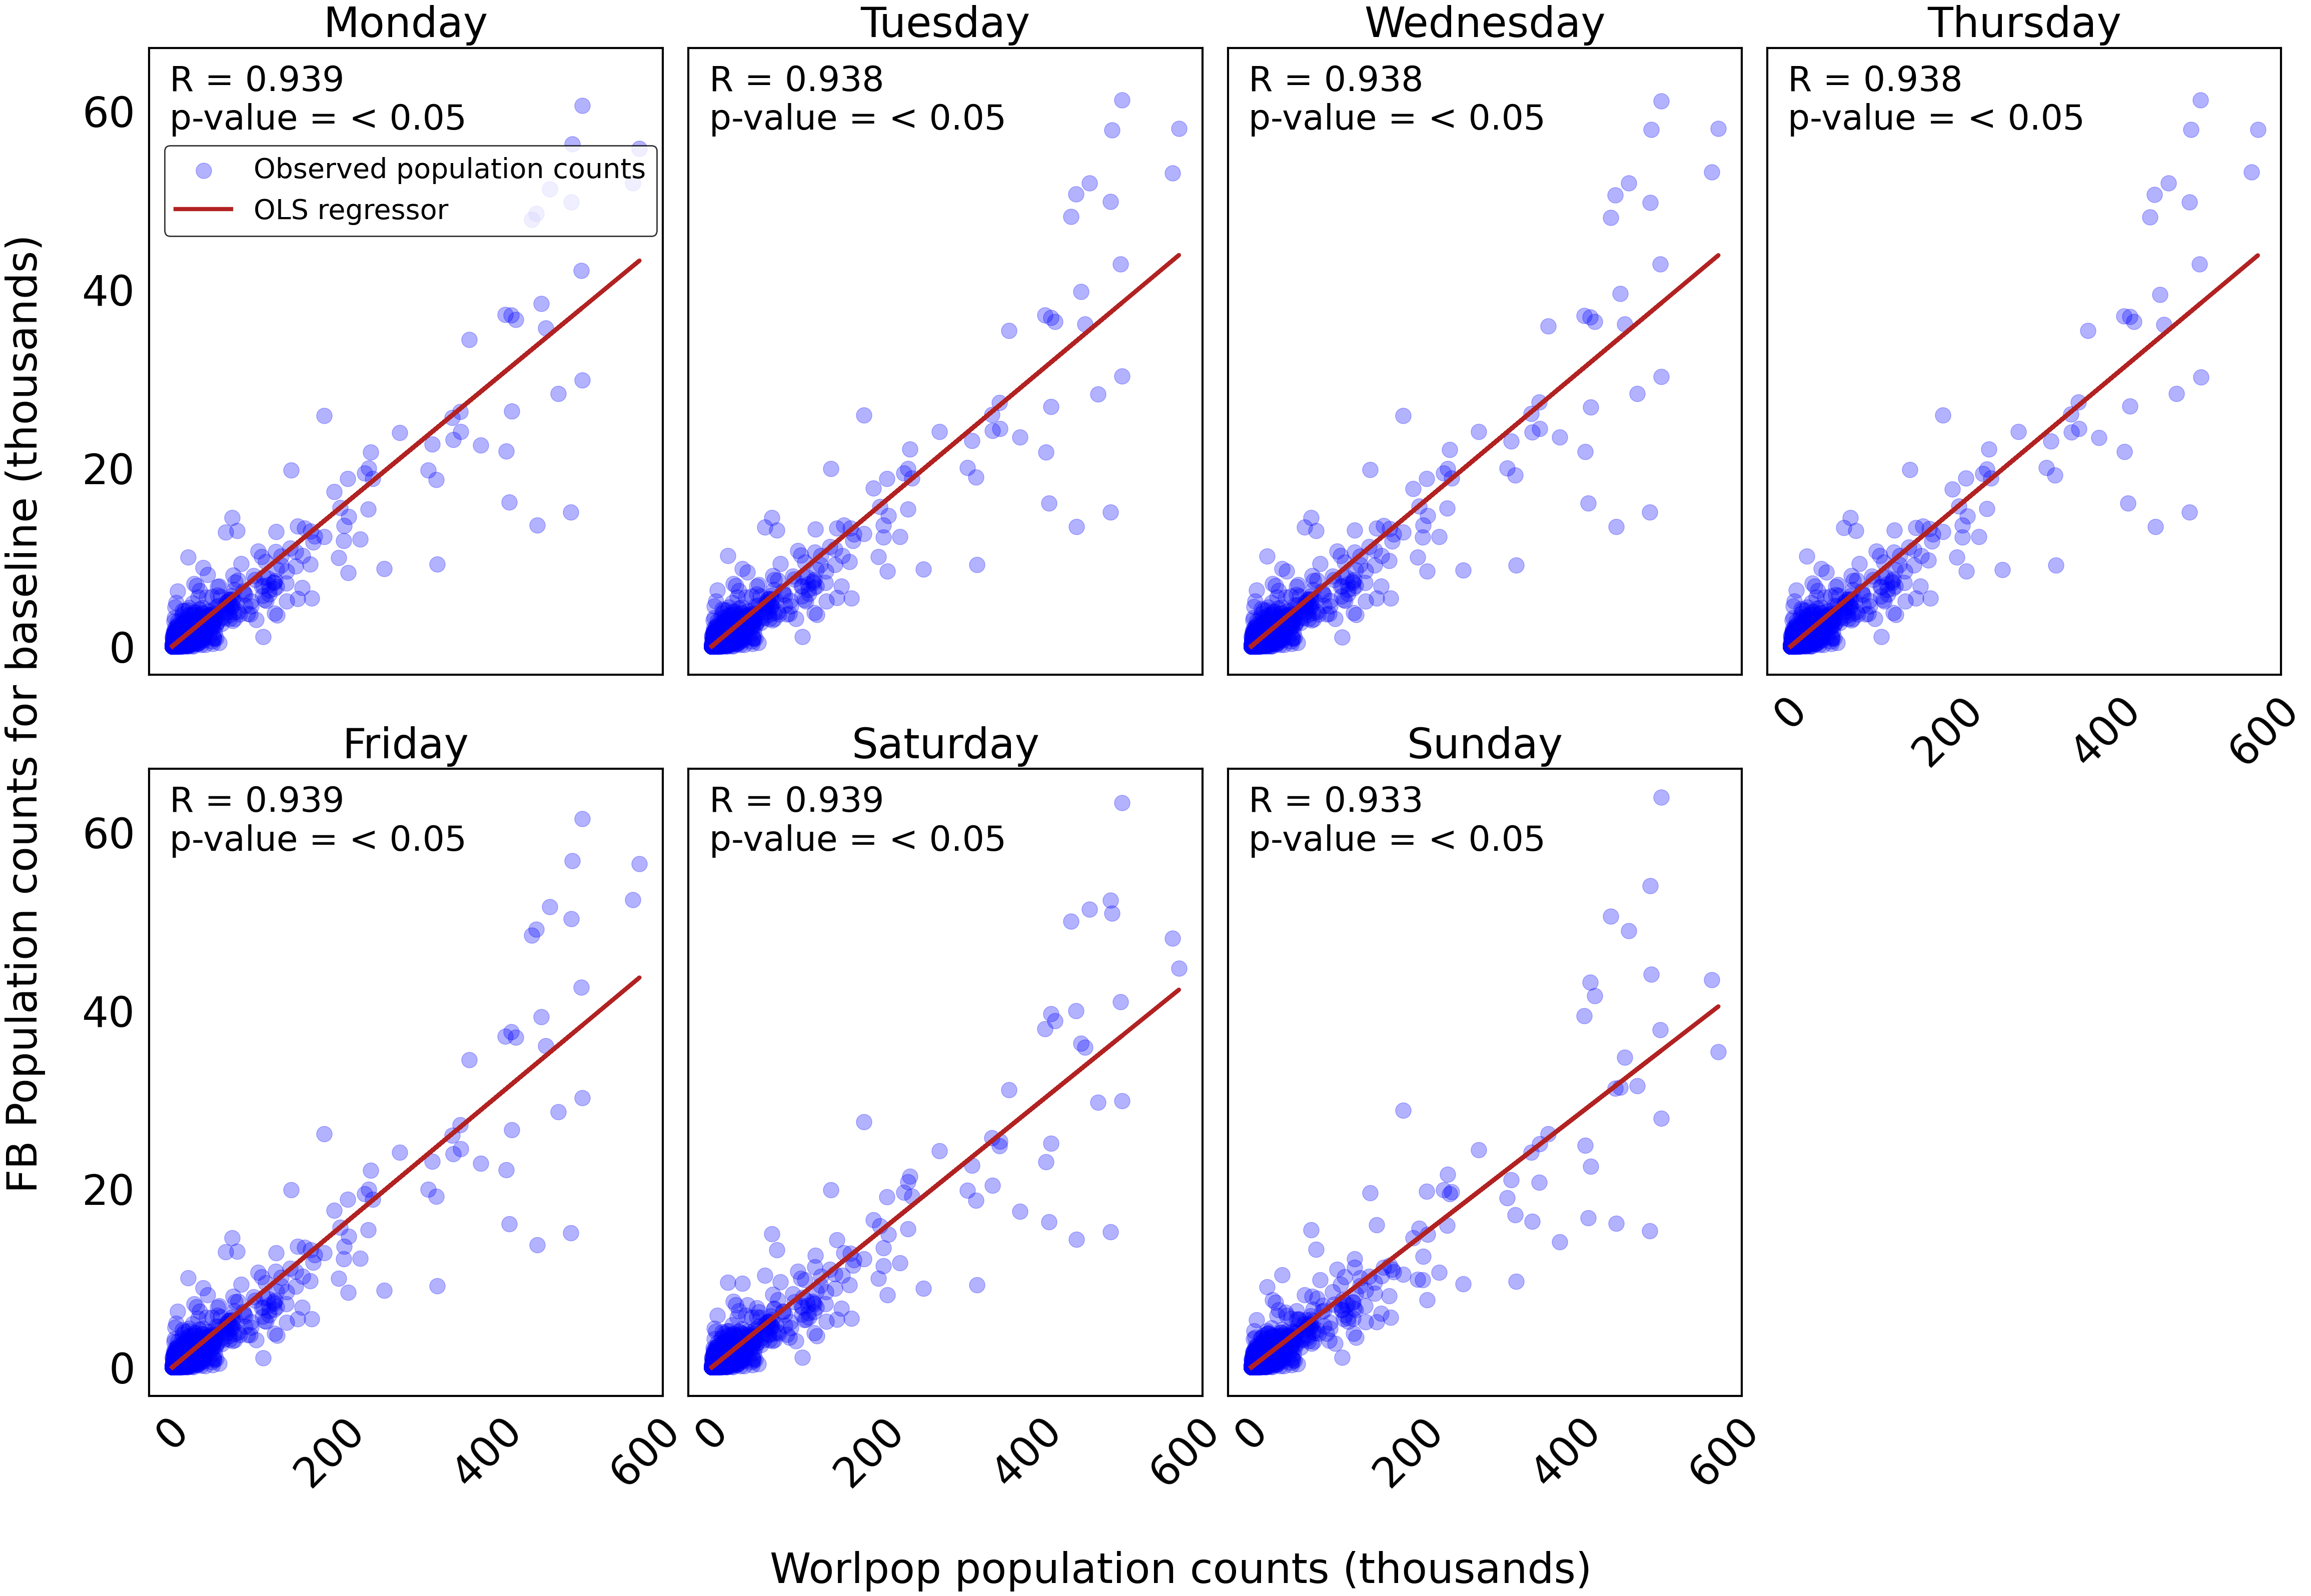
\includegraphics[width=\linewidth]{supplementary/correlation/correlation-wp-fb-pop-baseline-COL.png}
\caption{Correlation between Worldpop population counts and Facebook Population counts during the baseline period in Colombia, for each day of the week.}
\label{correlation-wp-fbpop-COL}
\end{figure}

\newpage

\subsection{Assessing results of spatial interaction model for imputing missing number of movements in baseline}

\begin{figure}[h!]
\centering
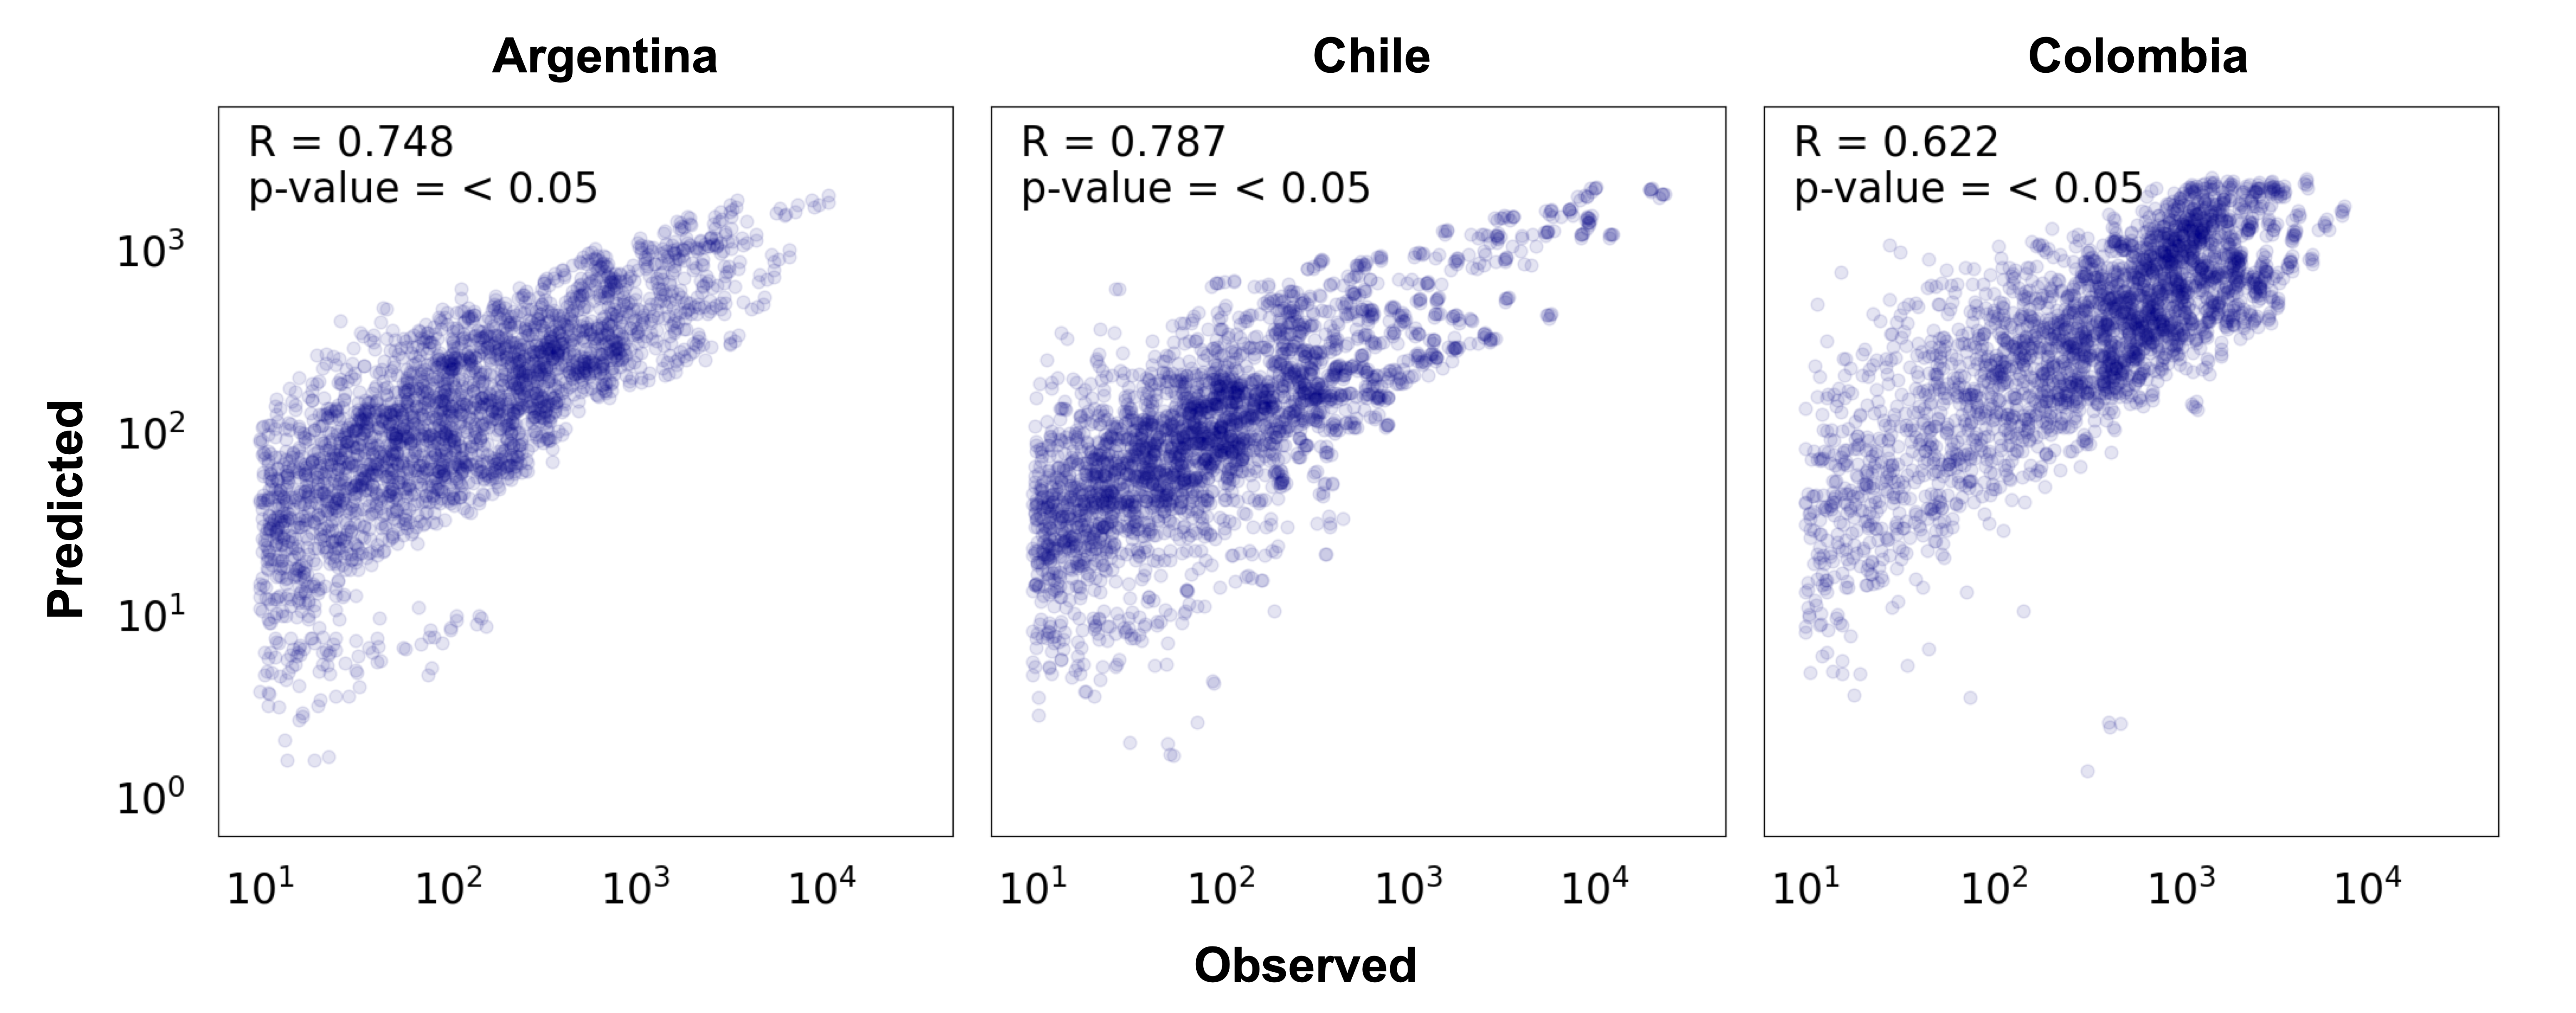
\includegraphics[width=\linewidth]{supplementary/sim/SF-sim-validation.png}
\caption{Relationship between observed and predicted value of number of movements between origin-destination pairs of Bing tiles during the baseline, for all weekdays.}
\end{figure}

\begin{figure}[h!]
\centering
\includegraphics[width=\linewidth]{supplementary/sim/SF-sim-check.png}
\caption{Relationship between Facebook Population at the origin and the destination of each population flow during the baseline period. The Facebook Population is considered after the imputation of the Facebook Population baseline data. The colour of the markers represents the volume of the flows during the baseline period, both observed and predicted through the spatial interaction model. Note that the Bing tiles used to record Facebook Movement data in Colombia are smaller than in Argentina and Chile, hence the lower numbers. }
\end{figure}

\newpage

\subsection{Sensitivity to flow imputation at two points in time}

\begin{figure}[h!]
\centering
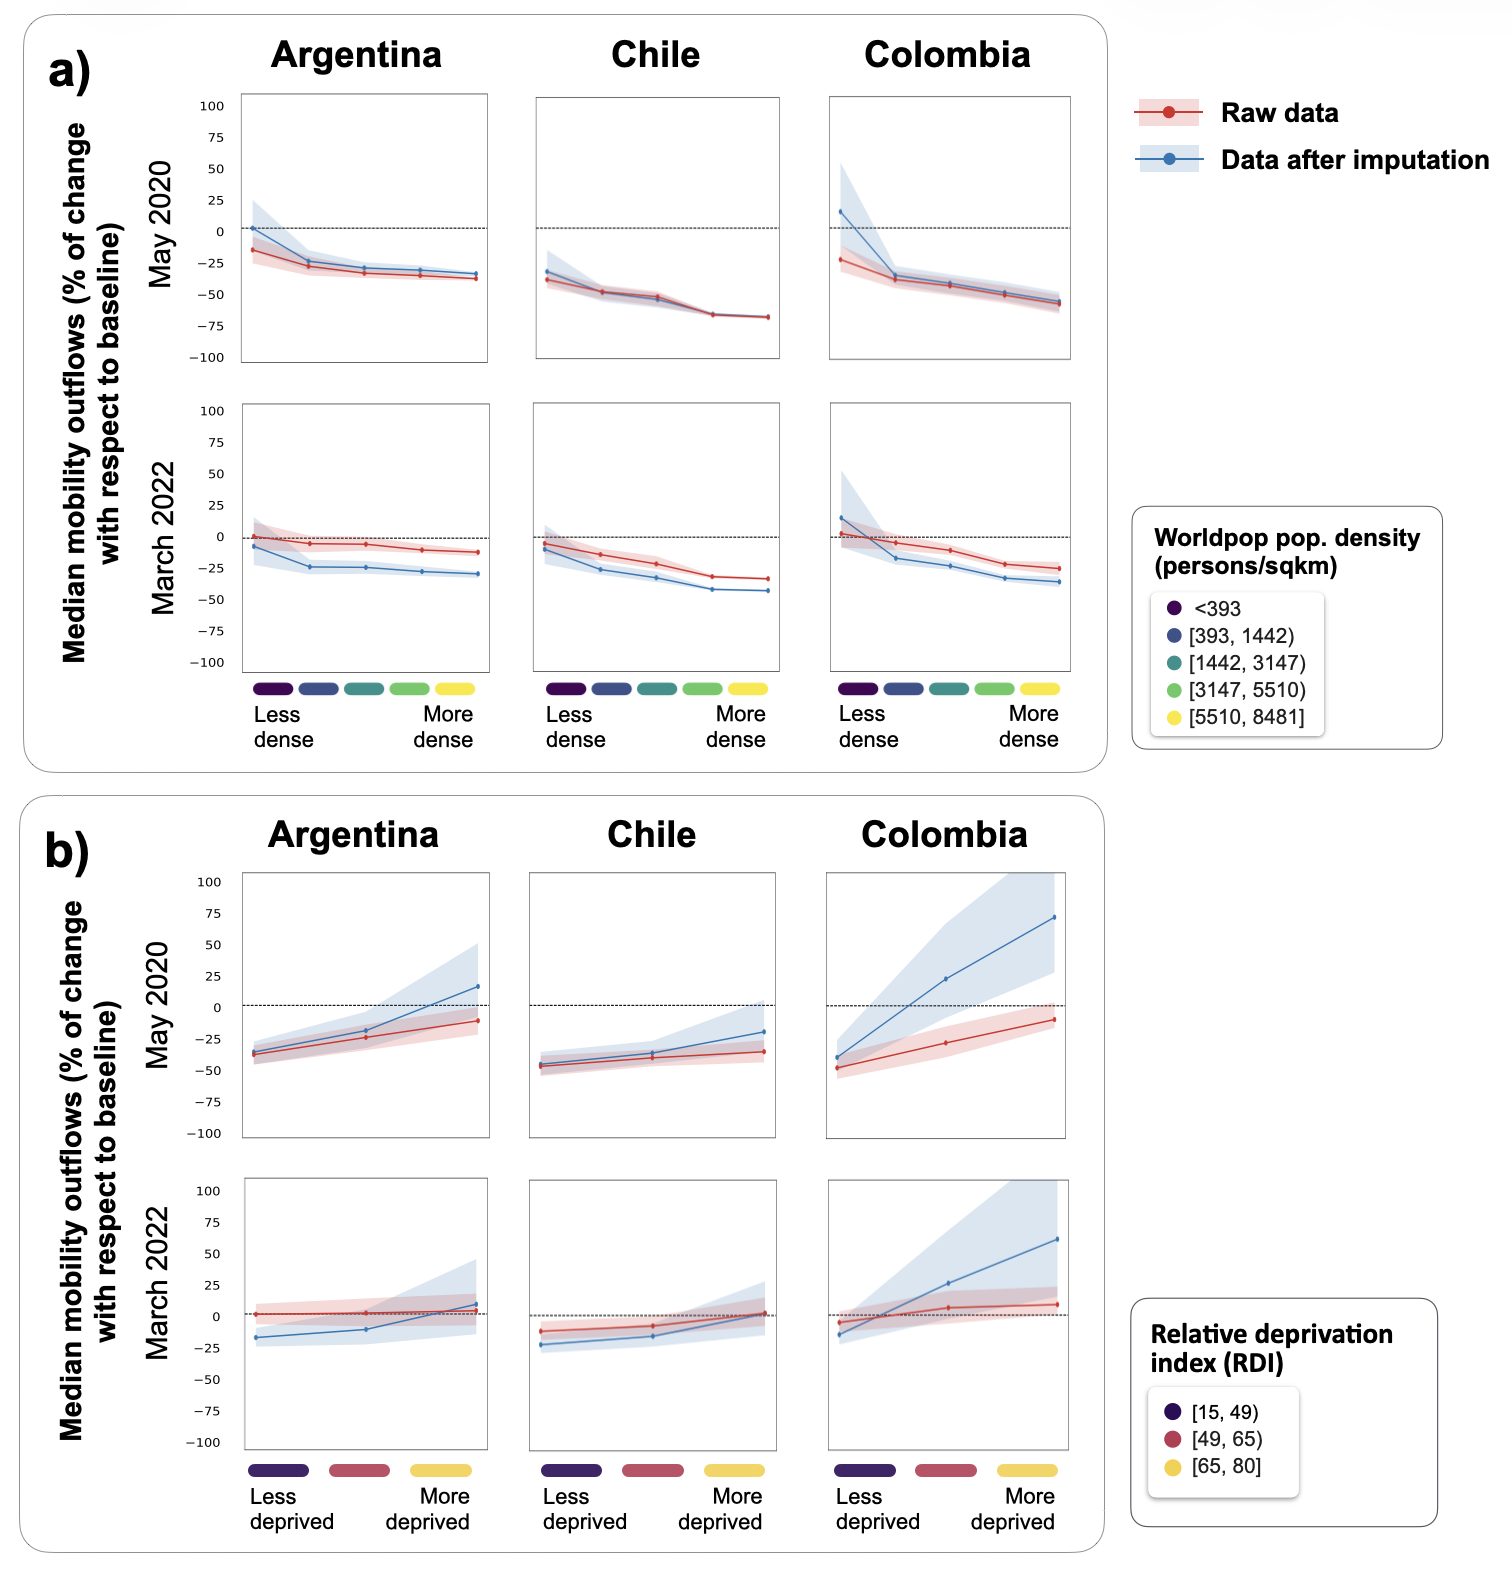
\includegraphics[width=\linewidth]{supplementary/validation-imputation/SF-validation-imputation-r2-censored10.png}
\caption{Comparison of raw and imputed mobility outflows at two time points in time, May 2020 and March 2022, across population-density and deprivation categories. Median mobility outflows, expressed as percentage change relative to the pre-pandemic baseline are shown for Argentina, Chile and Colombia using raw data and data after imputation. Panel (a) shows results by population-density category and panel (b) by relative deprivation index (RDI) category. Lines indicate the median across spatial units within each category, and shaded areas indicate the interquartile range (25th-75th percentiles).}
\end{figure}


\newpage
\section{Classification of tiles according to level of urbanisation and socioeconomic deprivation}

\begin{table}[h!]
\centering
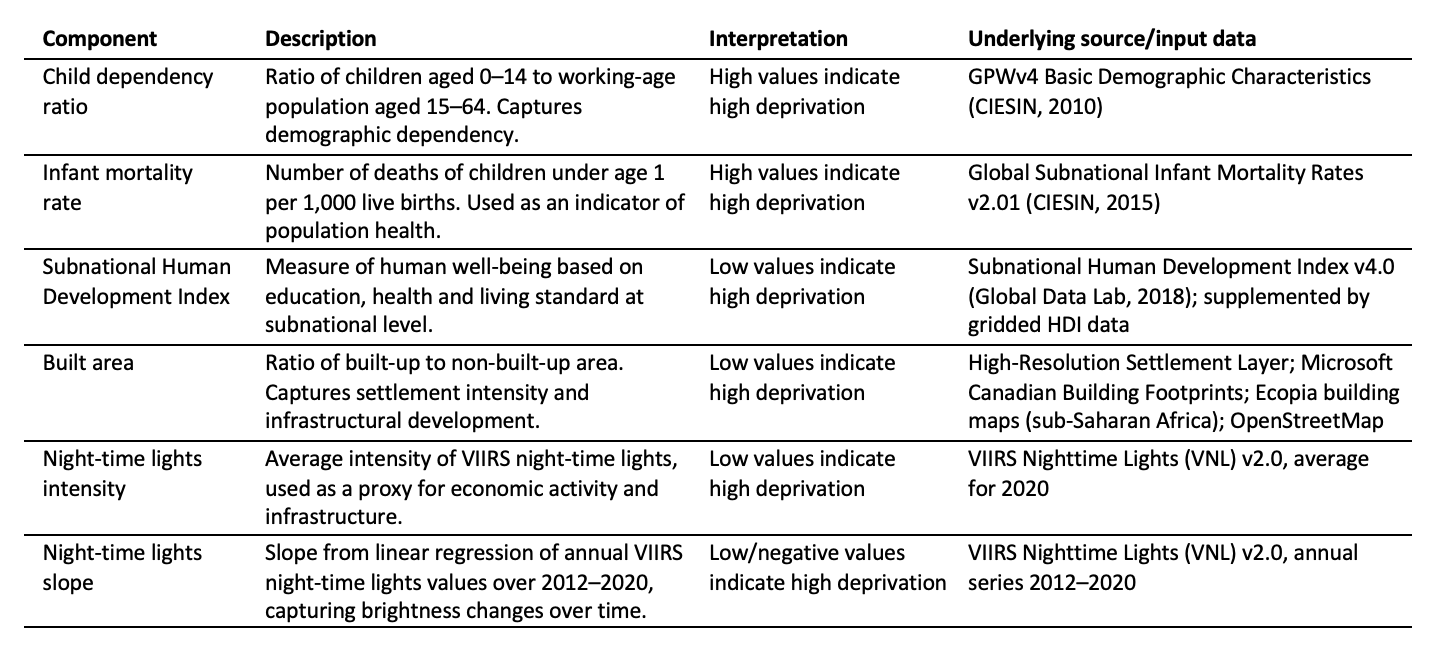
\includegraphics[width=\linewidth]{supplementary/categories/SF-rdi-components.png}
\caption{Variables and input data used in the construction of the Global Gridded Relative Deprivation Index (GRDIv1). The table reports the six component dimensions used by NASA SEDAC \cite{RDI2022} to compute the index, together with their definitions, interpretation in relation to deprivation and original source datasets. For the construction of the index, the variables were spatially harmonised and combined into a composite measure of relative deprivation at approximately 1 km resolution. Full methodology for index construction is explained in NASA's documentation \cite{RDI2022}. In the present study, the resulting RDI values were used to classify areas into low, medium and high deprivation categories.}
\end{table}

\begin{figure}[h!]
\centering
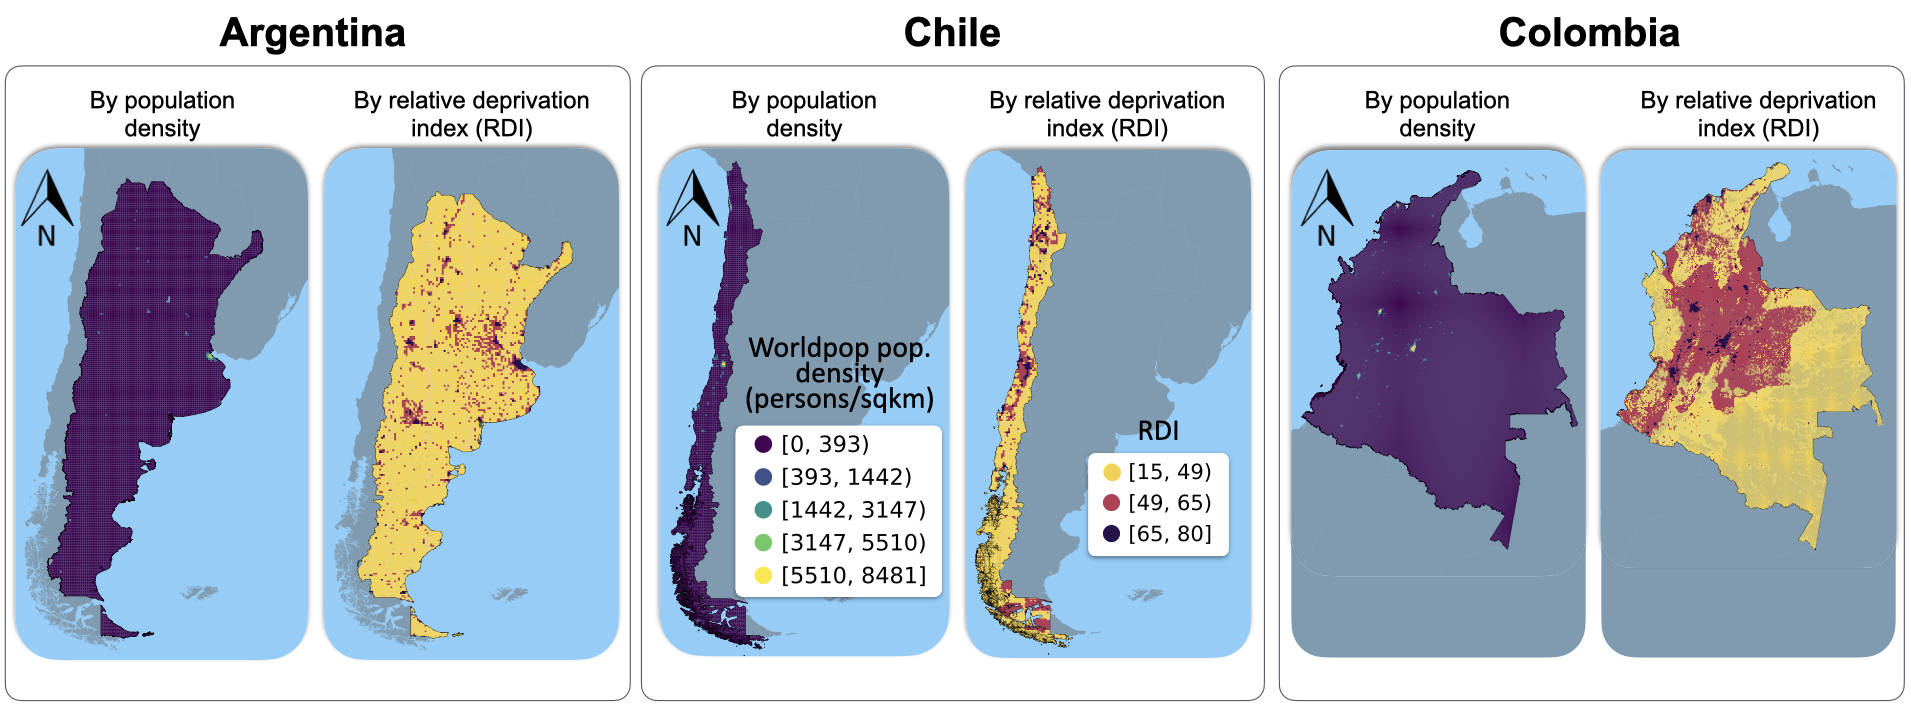
\includegraphics[width=\linewidth]{supplementary/categories/SF-maps-classes-r1.png}
\caption{Classification of spatial units into categories by population density and by relative deprivation index. This figure provides descriptive context for the key socioeconomic and density categories used in the analysis.}
\end{figure}

\begin{figure}[h!]
\centering
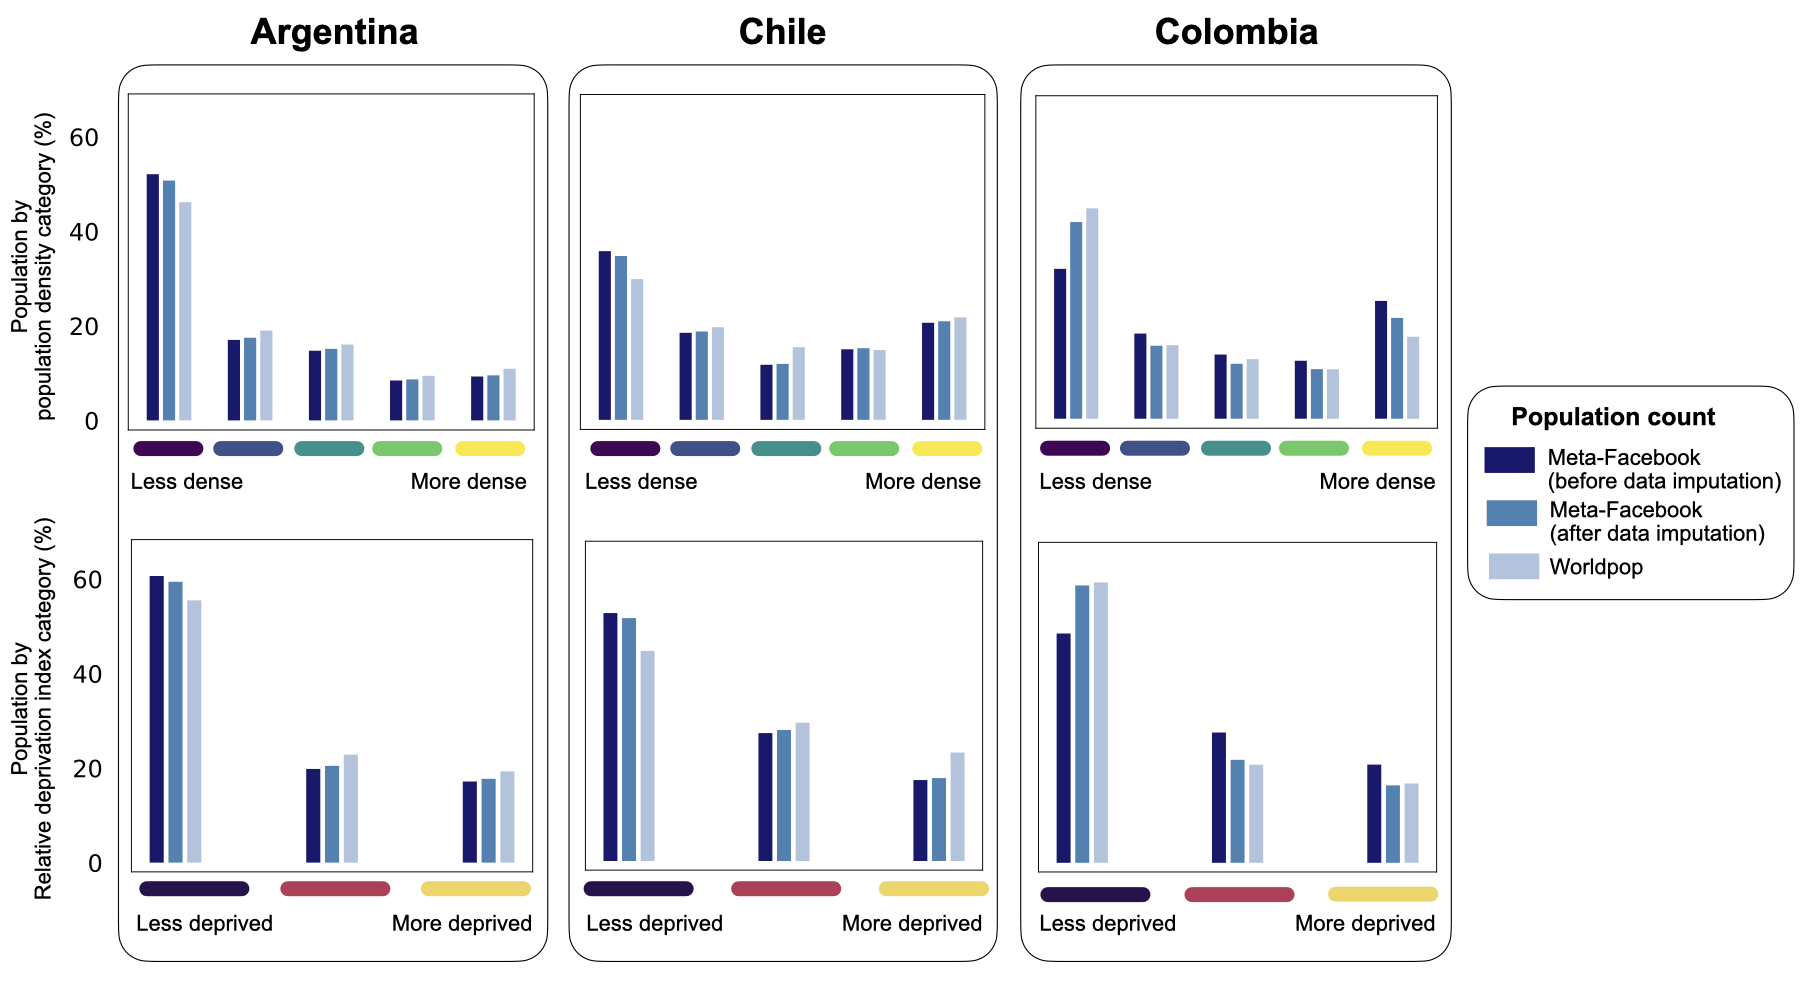
\includegraphics[width=\linewidth]{supplementary/categories/SF-classes-bias-r1.png}
\caption{Population share in each population density and Relative Deprivation Index category by country, according to Meta-Facebook data (before and after imputation) and to Worldpop data. The similarity in category-specific population shares across the Facebook and Worldpop indicates that the Meta-Facebook data provide reasonably representative coverage across deprivation categories, particularly after imputation.}
\end{figure}

\begin{figure}[h!]
\centering
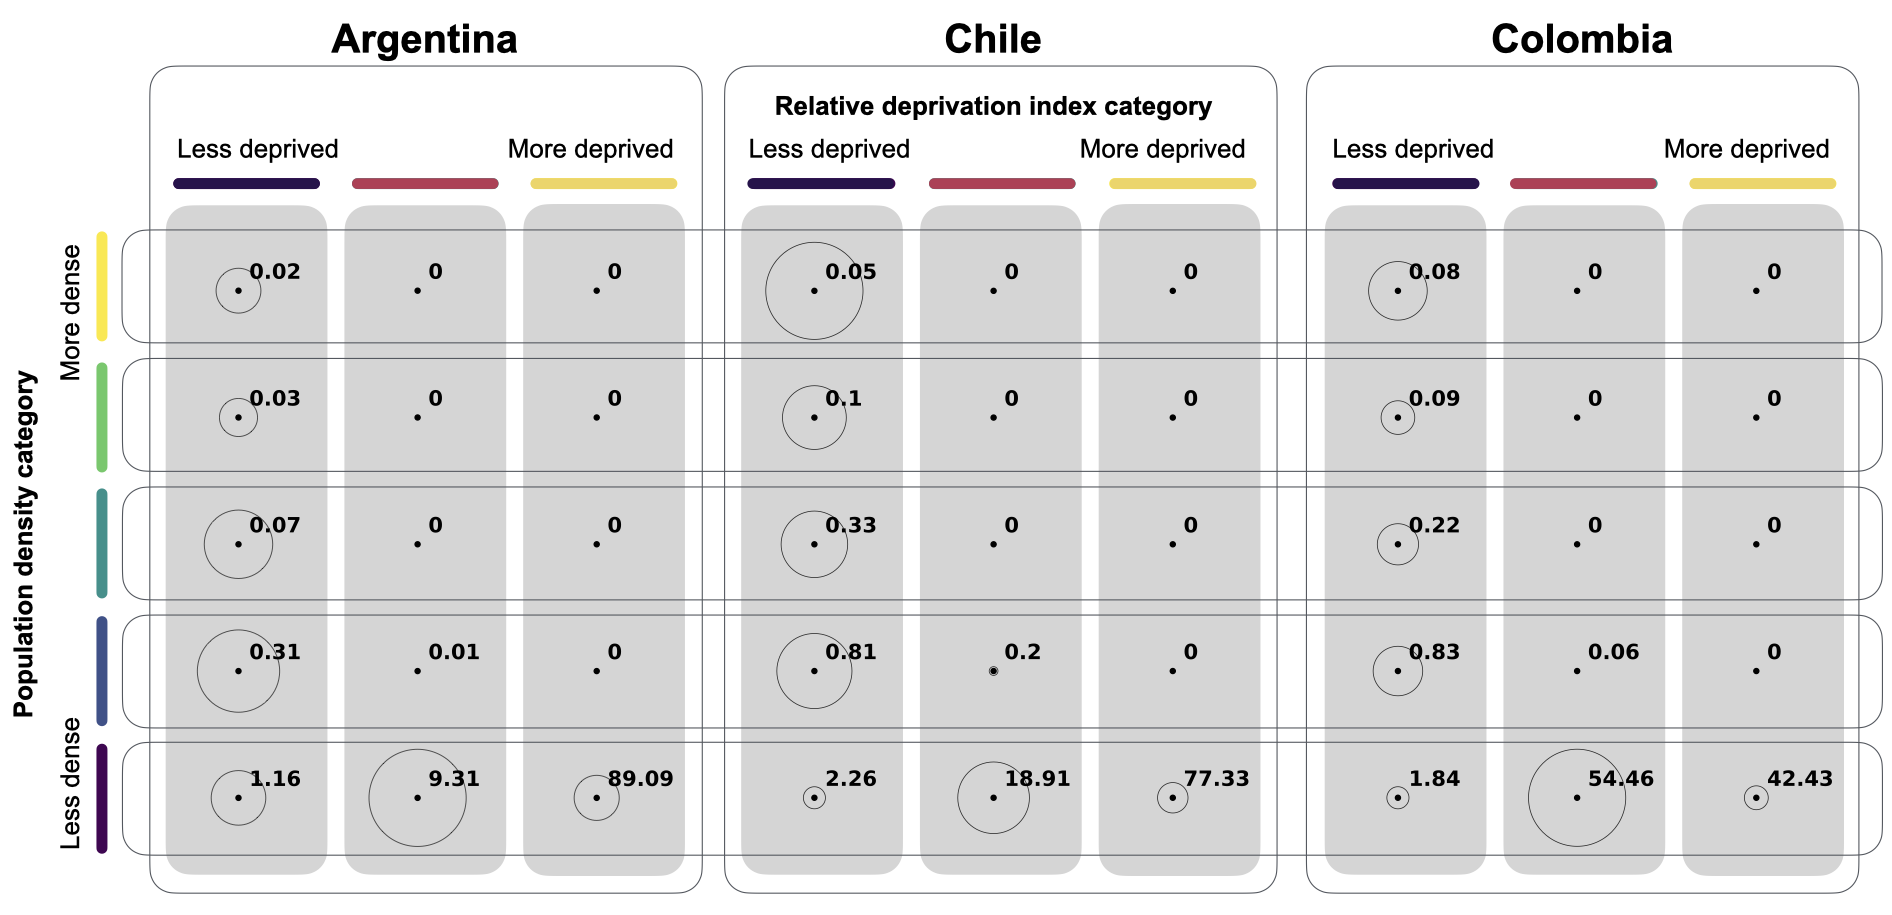
\includegraphics[width=\linewidth]{supplementary/categories/SF-classes-combined-r1.png}
\caption{Joint distribution of spatial units by population density (rows) and relative deprivation index (RDI) categories (columns), with values representing the percentage of spatial units within each country. Circle sizes indicate the total population corresponding to each category pair. This figure provides descriptive context for the combined socioeconomic and density structure of the study areas.}
\end{figure}

\clearpage
\section{Trend analysis}

\subsection{Time series to be modelled with trend analysis}

\begin{figure}[h!]
\centering
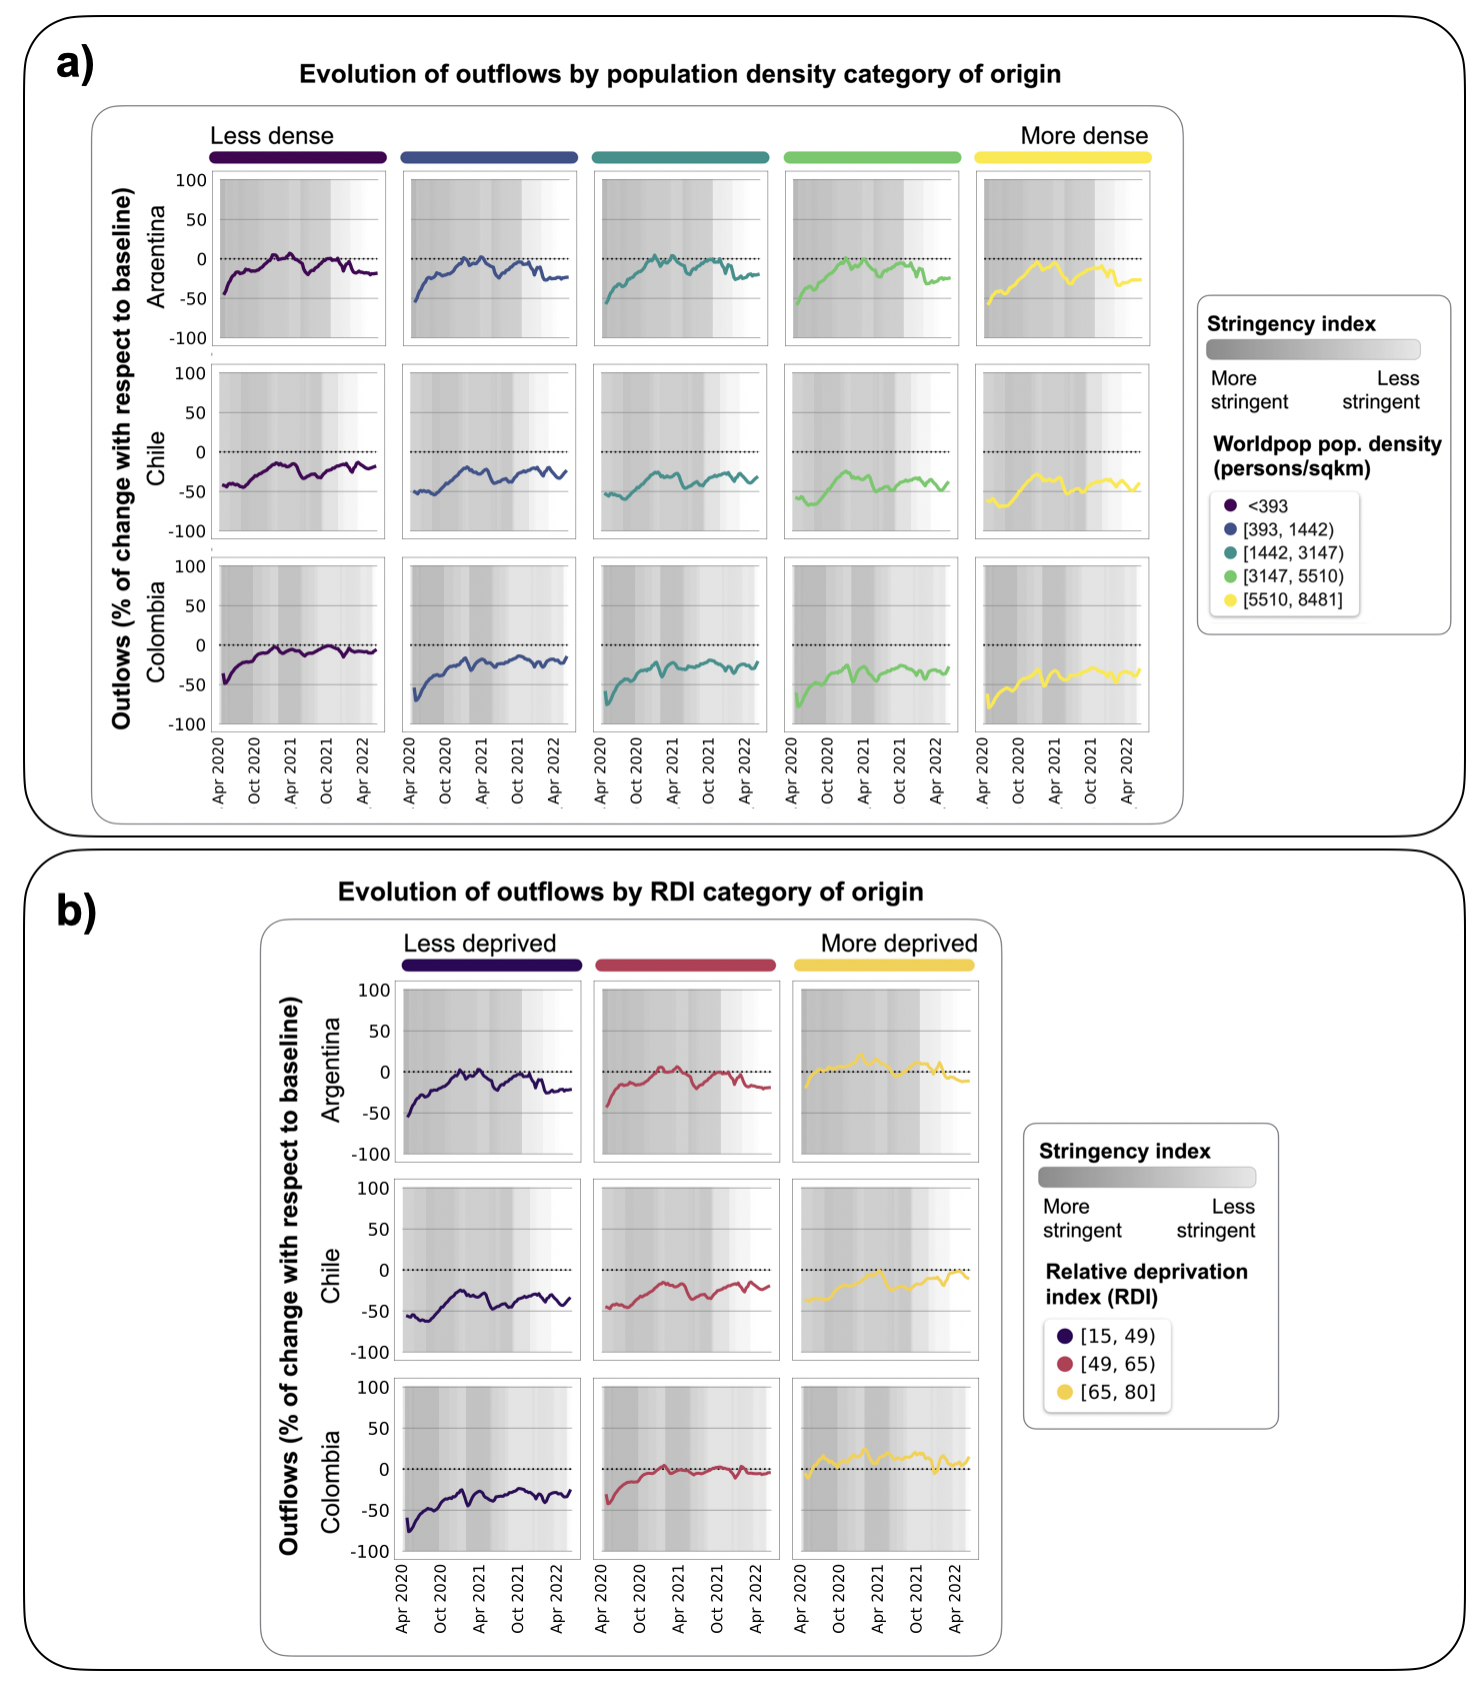
\includegraphics[width=0.8\linewidth]{supplementary/time-series/Fig-recovery-combined-design-r2.png}
\caption{Time evolution of percentage change of outflows relative to pre-pandemic baseline levels, by country and by (a) population density category and (b) relative deprivation category.}
\label{fig-classification}
\end{figure}

\clearpage
\subsection{Robustness of trend extraction method}

\begin{table}[h!]
\centering
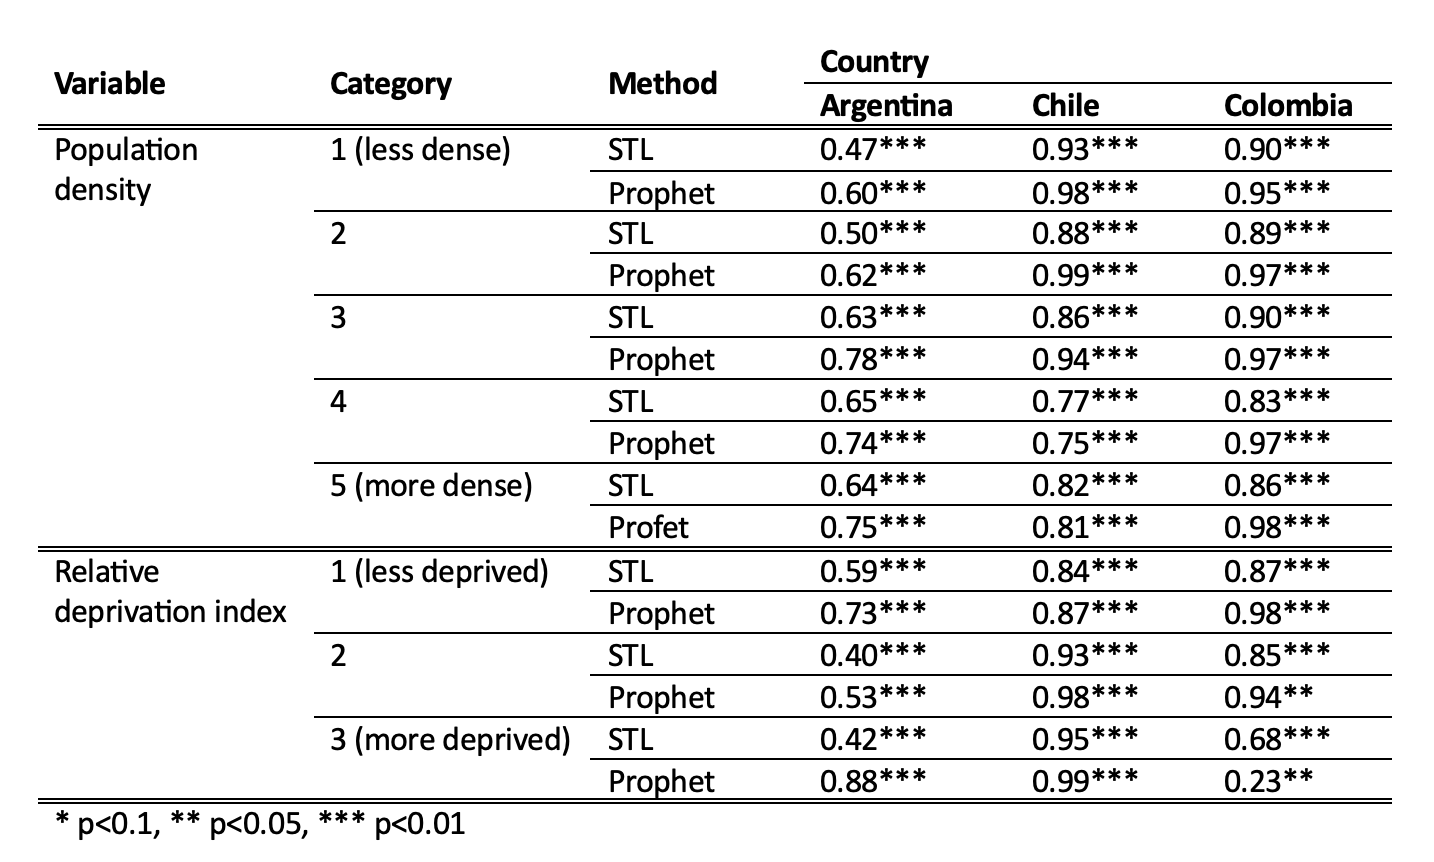
\includegraphics[width=0.8\linewidth]{supplementary/trend-extraction/trend-extraction-robustness-r2.png}
\caption{Pearson correlation coefficients (with p-values) comparing trends extracted using the moving-average method (used in the main analysis) with those extracted using Seasonal-Trend decomposition using Loess (STL) decomposition and the Prophet model. Results are reported for each country and across all population density and relative deprivation categories. The high correlations indicate strong consistency across trend extraction methods.}
\end{table}


\subsection{Model specification}

\begin{table}[h!]
\centering
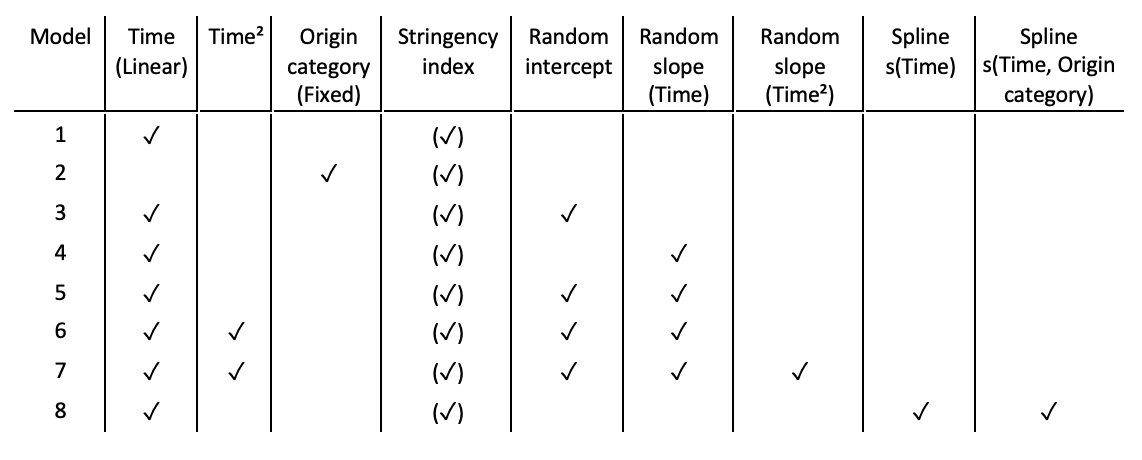
\includegraphics[width=0.8\linewidth]{supplementary/models-tables/SF-models-specification.png}
\caption{Summary of model specifications. There is a total of 16: 14 for mixed-effects, 2 for Generalised Additive Models with spline terms. Each row in the table represents a pair of models: one that includes the stringency index as a covariate and one that excludes it. This is denoted by a bracketed check mark [(\checkmark)]. All other check marks [\checkmark] indicate terms that are included in both models of the pair. Random effects and the second spline term are considered according to the population density or the Relative Deprivation Index (RDI) of the origin location of outflows.}
\end{table}



\newpage
\subsection{Mixed-effects model outcomes by old-age dependency ratio categories}

\begin{figure}[h!]
\centering
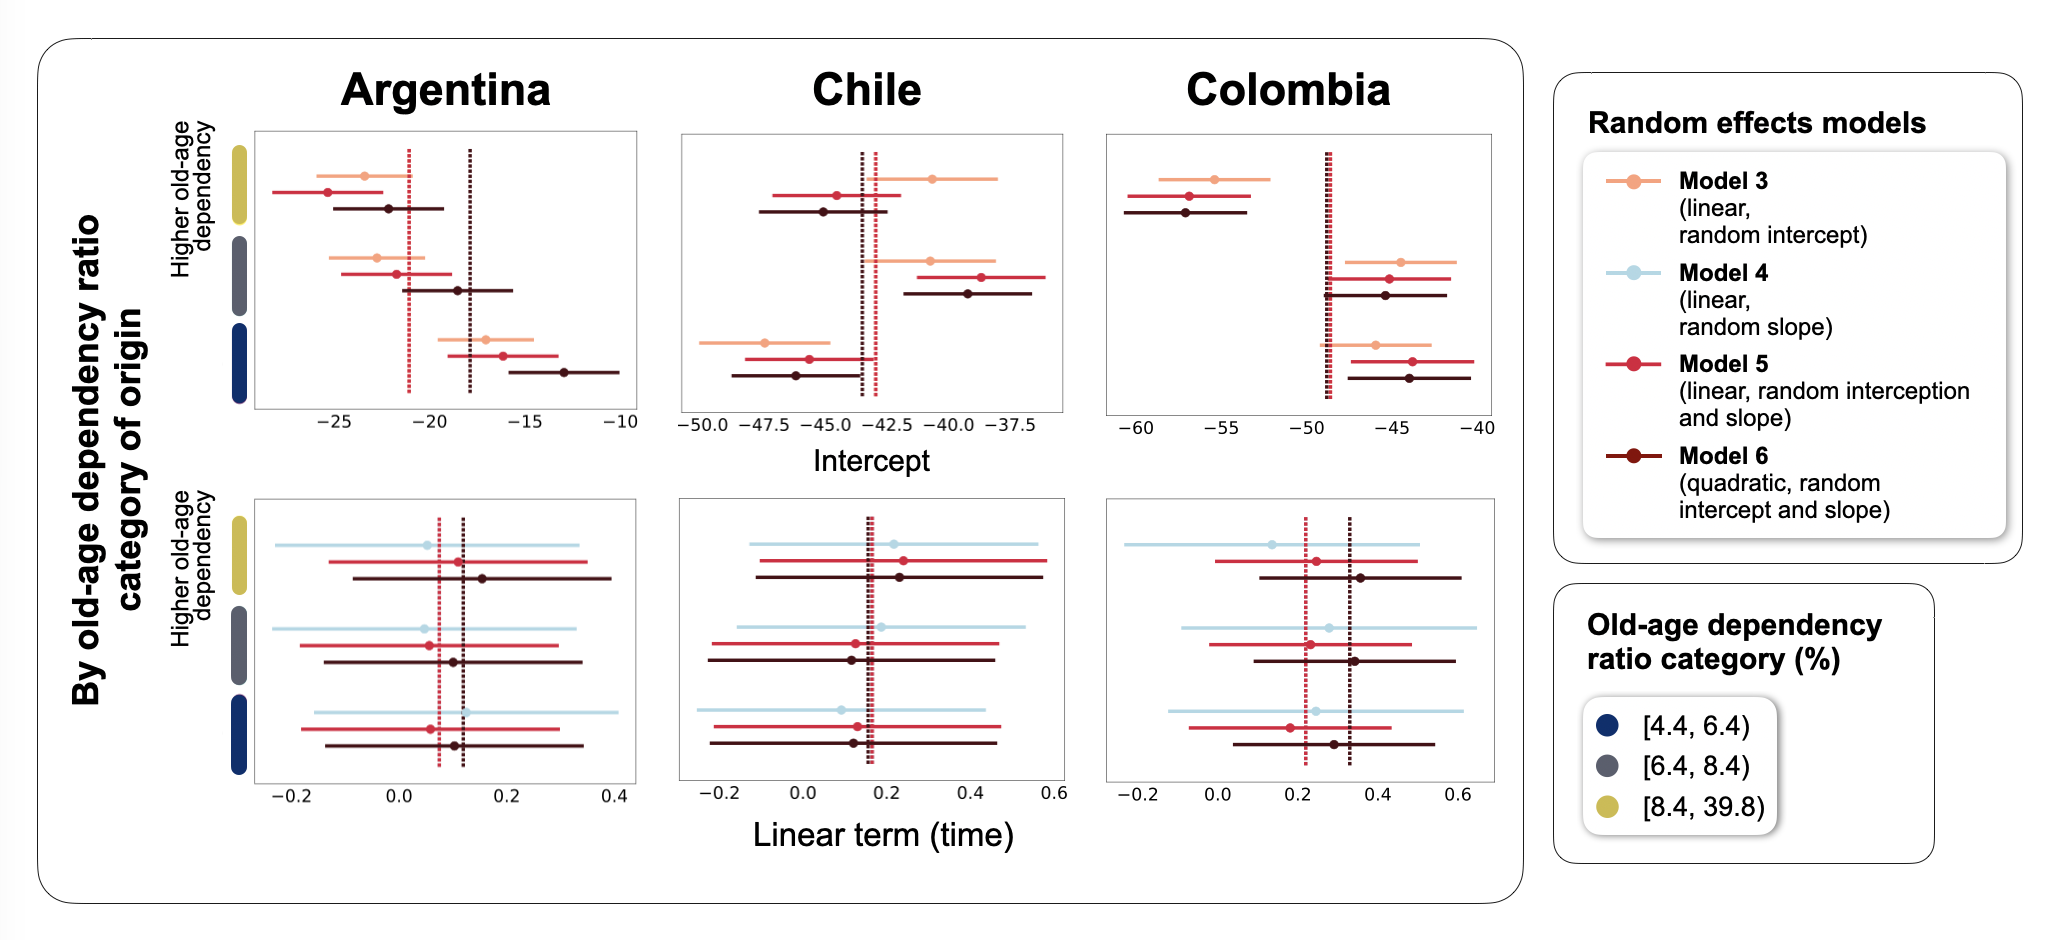
\includegraphics[width=\linewidth]{supplementary/models-figures/SF-re-combined-design-oldage-r2.png}
\caption{Mixed-effects modelling estimates (random intercept and random
linear time term), by country and old-age dependency ratio category; bars denote 95\% confidence intervals; colours encode different model specifications; vertical dashed lines
represent the estimated values for fixed effects of the corresponding terms (i.e. intercept, linear time). Panel a) displays results by population density category and b) by relative
deprivation category.}
\end{figure}

\clearpage
\subsection{Model estimates - relative change in outflows}

\begin{table}[h!]
\centering
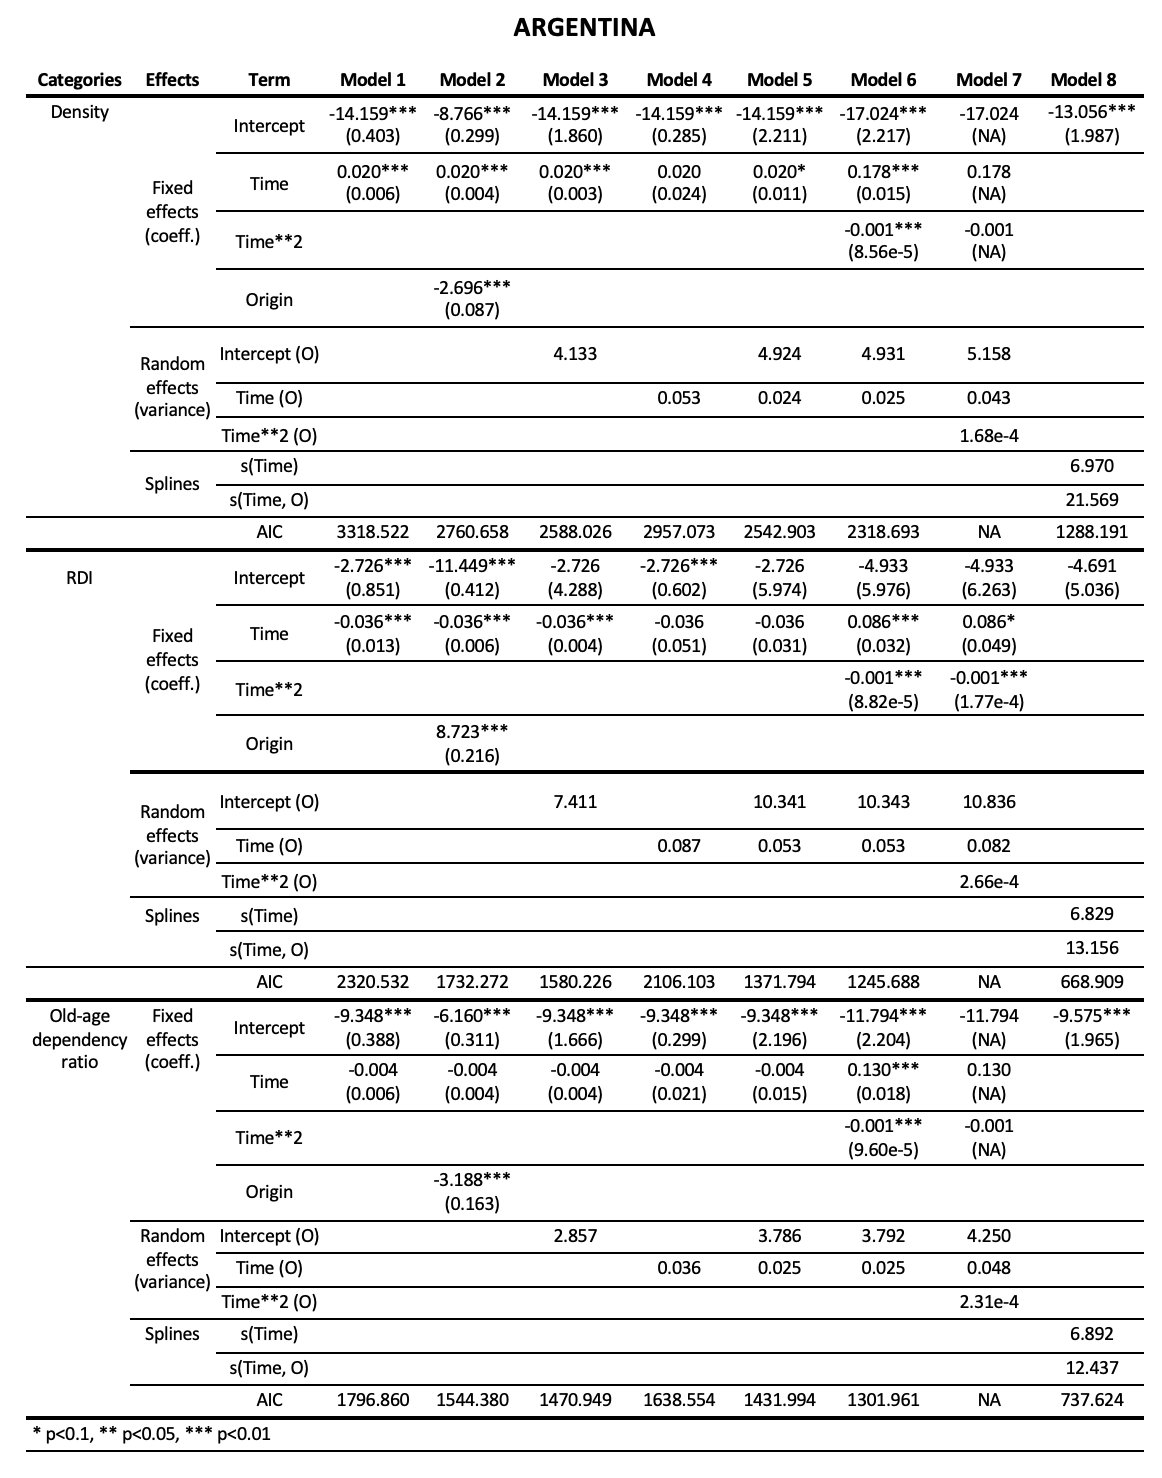
\includegraphics[width=0.9\linewidth]{supplementary/models-tables/models-table-ARG-quadratic-new-censored10.png}
\caption{Results of mixed-effects and Generalised Additive Model (GAM) models for trend analysis of relative change in outflows in Argentina. Fixed and random effects according to the population density, the Relative Deprivation Index (RDI) or the old-age dependency ratio of the origin location of outflows are reported for Models 1-7. Effective degrees of freedom are reported for the Spline terms in Model 8.}
\end{table}

\clearpage

\begin{table}[h!]
\centering
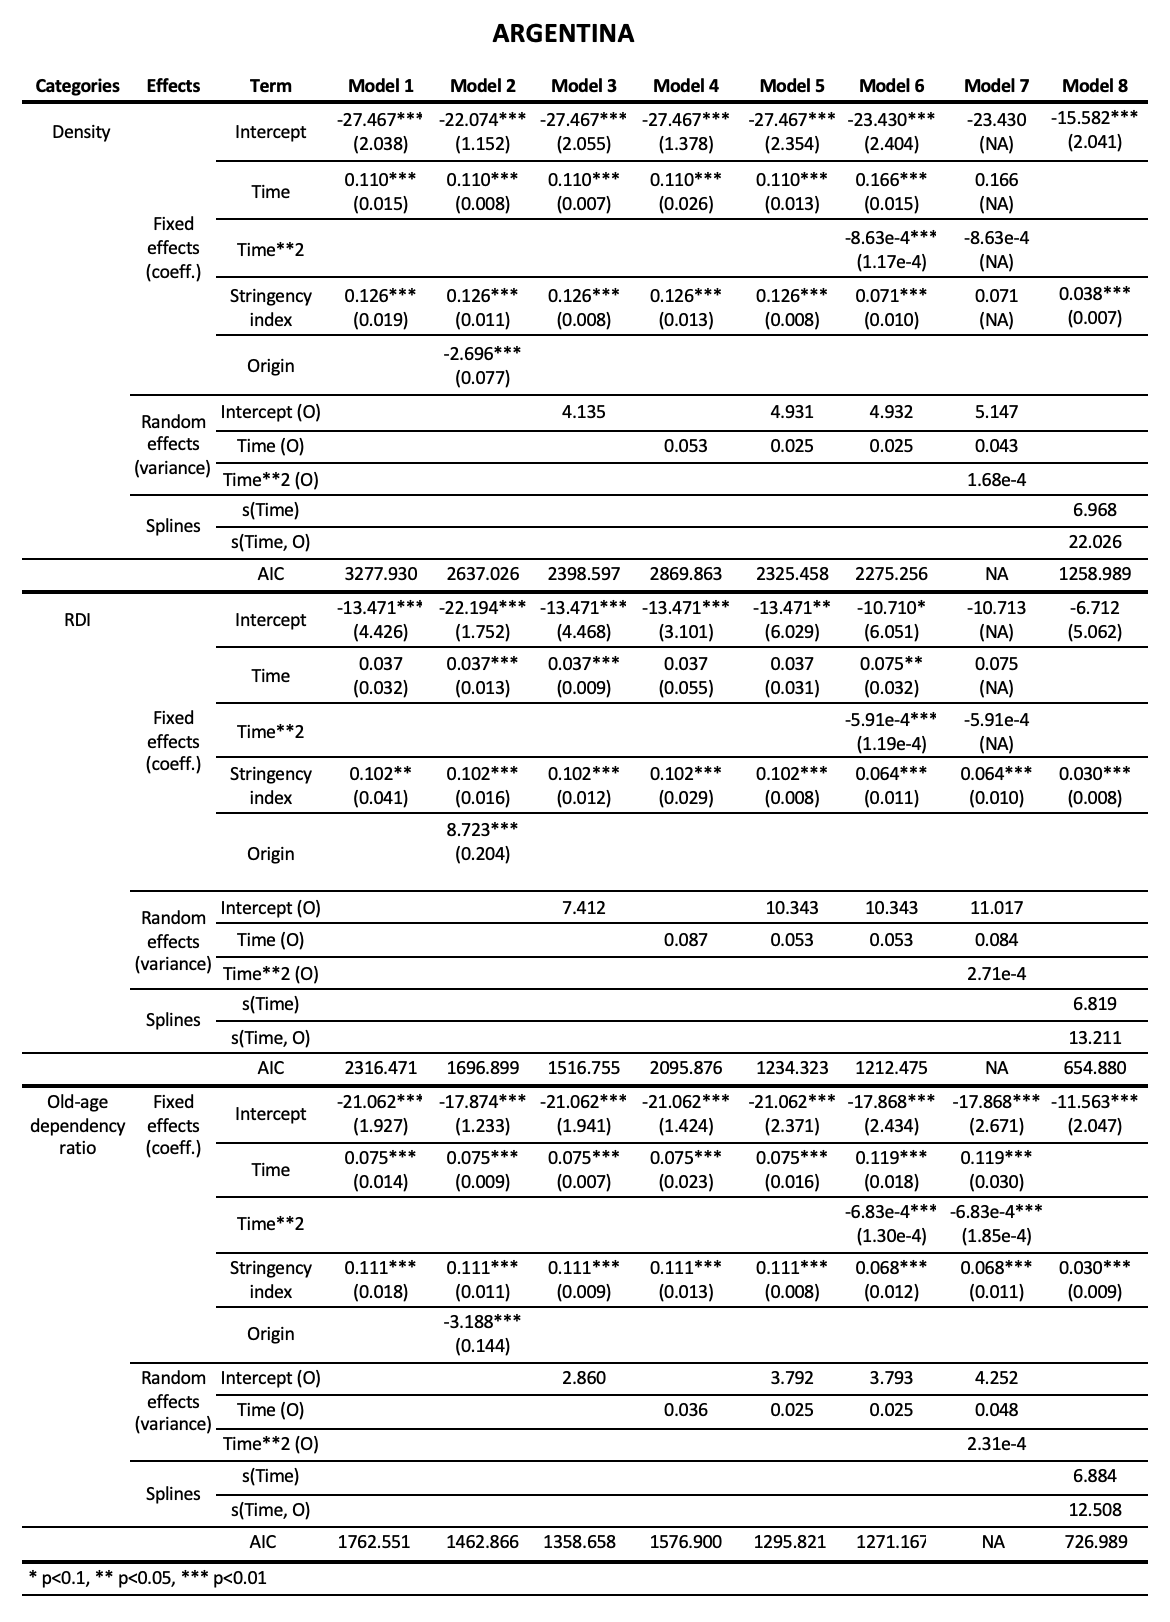
\includegraphics[width=0.9\linewidth]{supplementary/models-tables/models-table-ARG-quadratic-stringency-new-censored10.png}
\caption{Results of mixed-effects and Generalised Additive Model (GAM) models for trend analysis of relative change in outflows in Argentina including stringency index as a predictor variable. Fixed and random effects according to the population density, the Relative Deprivation Index (RDI) or the old-age dependency ratio of the origin location of outflows are reported for Models 1-7. Effective degrees of freedom are reported for the Spline terms in Model 8.}
\label{tab-modelsARG-stringency}
\end{table}

\clearpage

\begin{table}[h!]
\centering
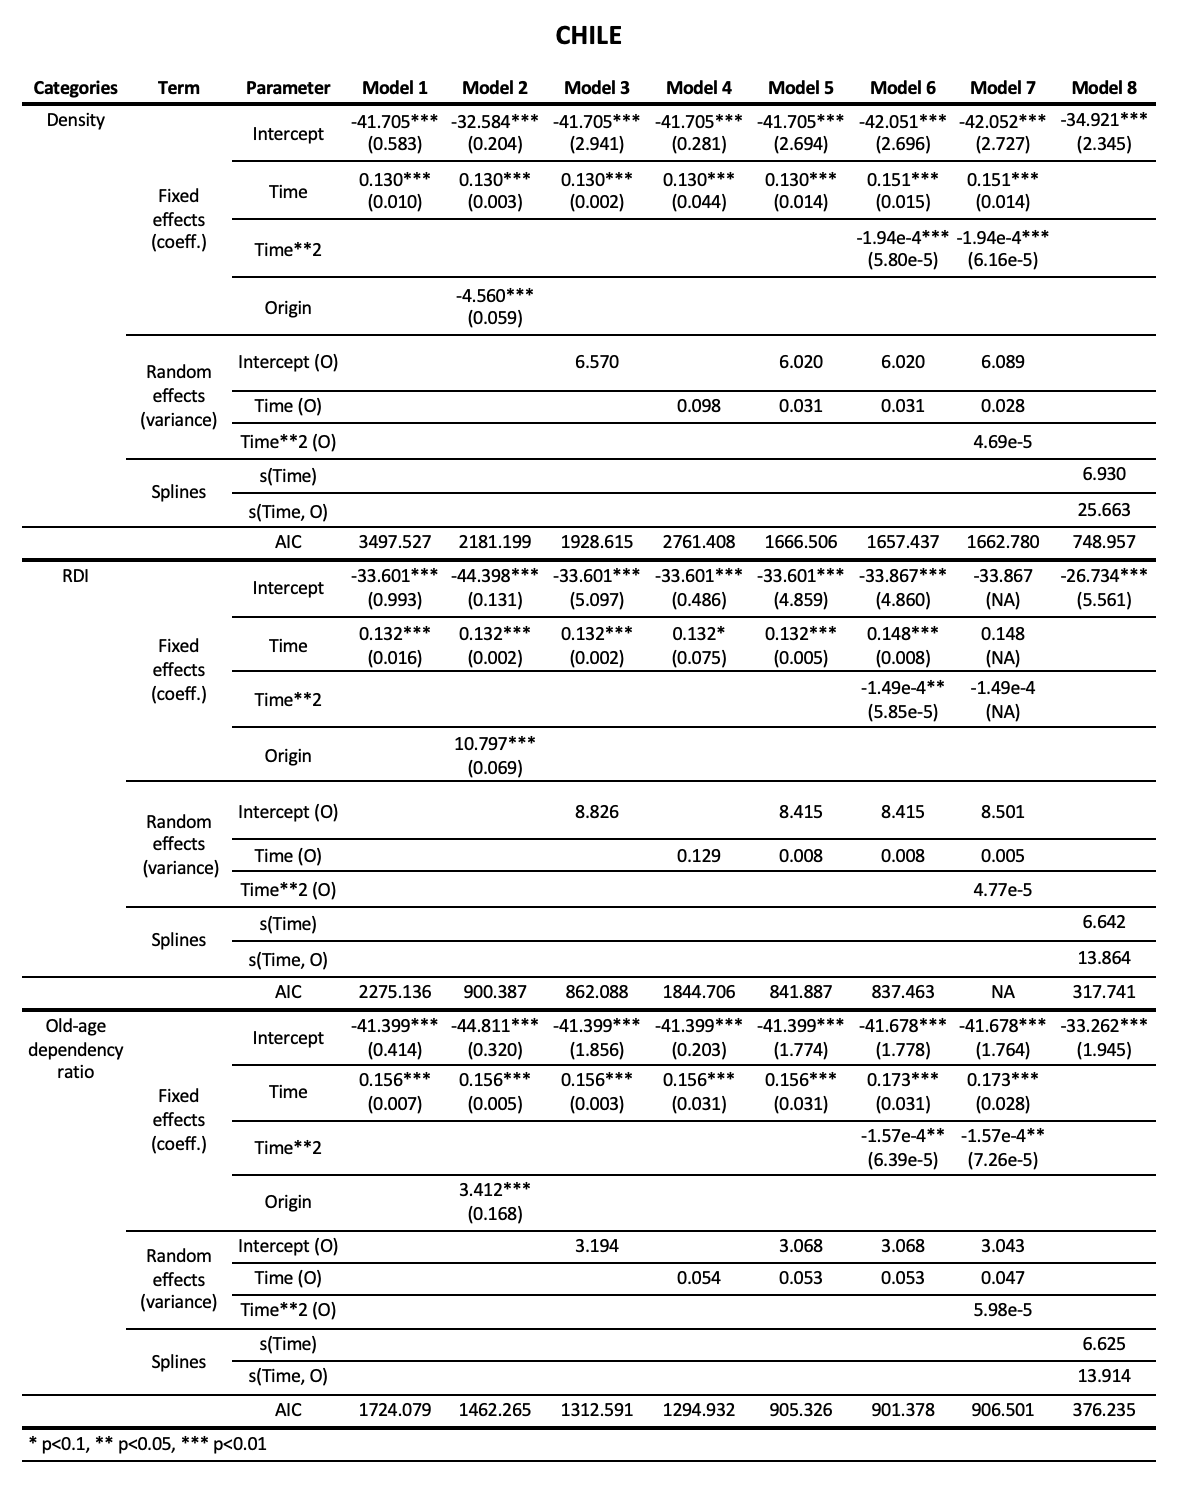
\includegraphics[width=0.9\linewidth]{supplementary/models-tables/models-table-CHL-quadratic-new-censored10.png}
\caption{Results of mixed-effects and Generalised Additive Model (GAM) models for trend analysis of relative change in outflows in Chile. Fixed and random effects according to the population density, the Relative Deprivation Index (RDI) or the old-age dependency ratio of the origin location of outflows are reported for Models 1-7. Effective degrees of freedom are reported for the Spline terms in Model 8.}
\label{tab-modelsCHL}
\end{table}

\clearpage

\begin{table}[h!]
\centering
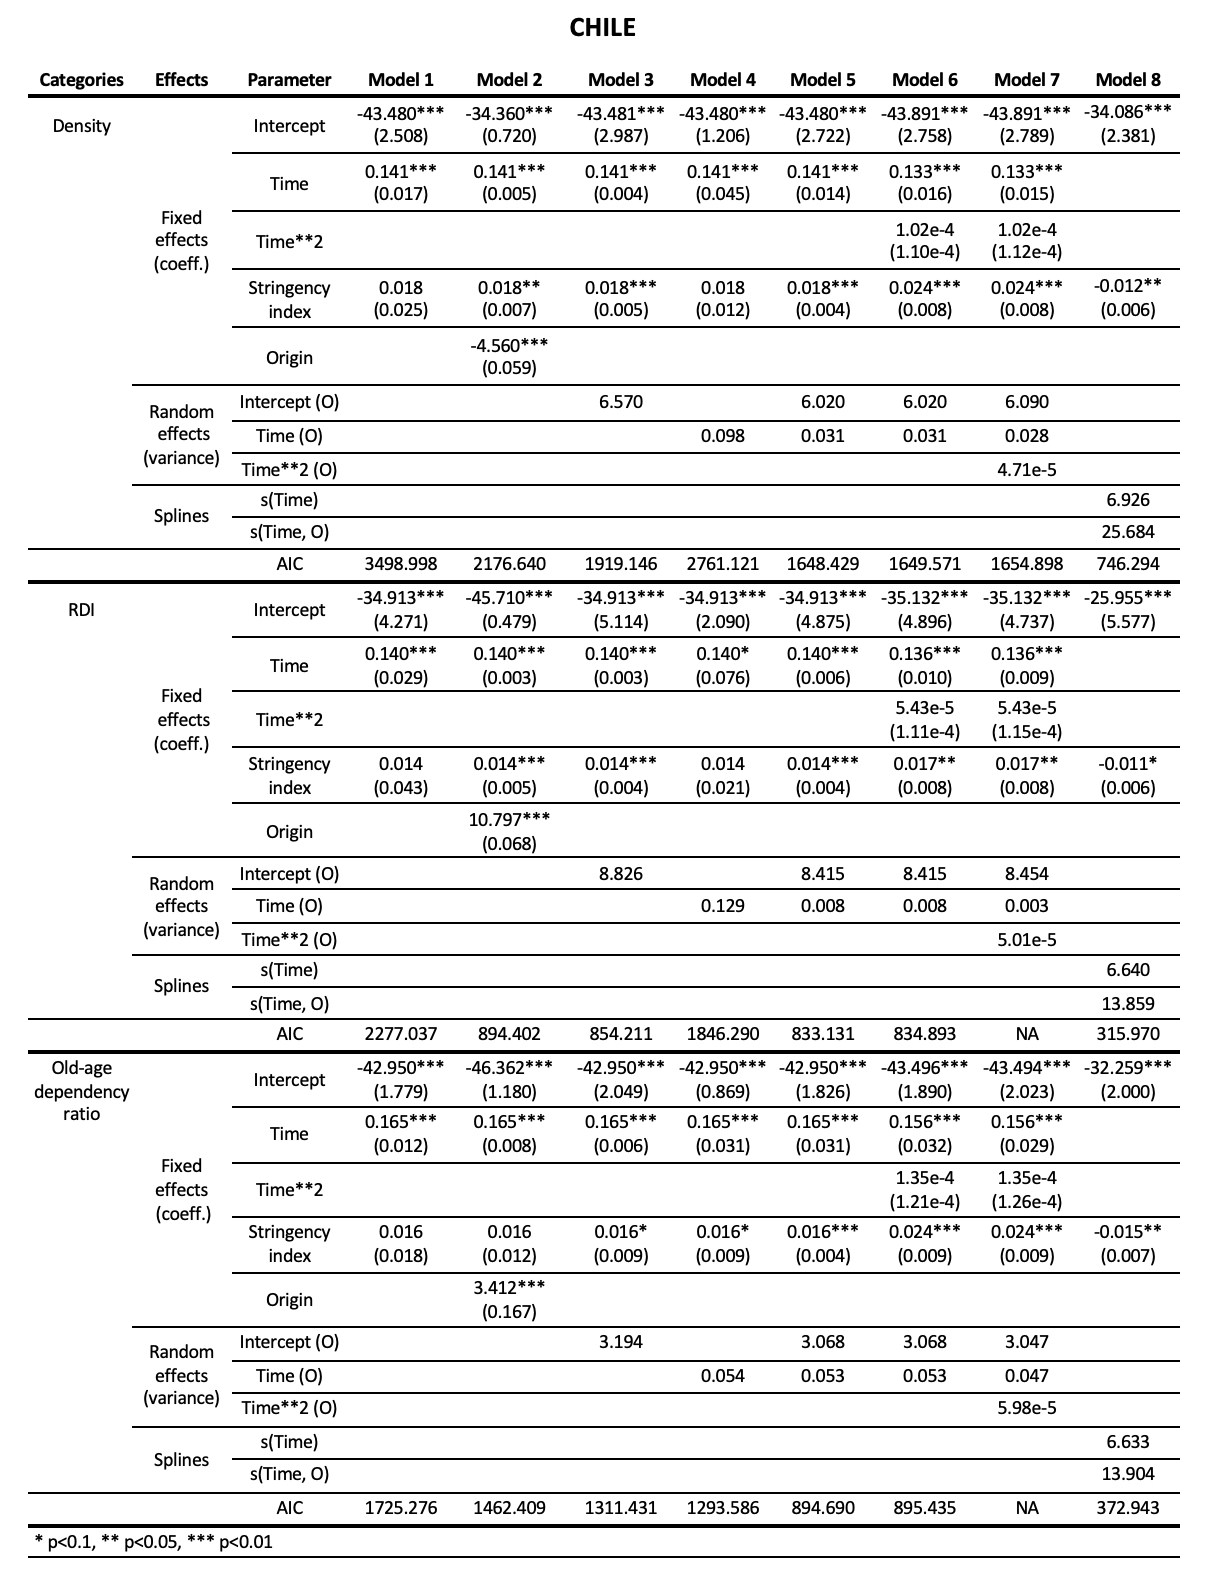
\includegraphics[width=0.9\linewidth]{supplementary/models-tables/models-table-CHL-quadratic-stringency-new-censored10.png}
\caption{Results of mixed-effects and Generalised Additive Model (GAM) models for trend analysis of relative change in outflows in Chile including stringency index as a predictor variable. Fixed and random effects according to the population density, the Relative Deprivation Index (RDI) or the old-age dependency ratio of the origin location of outflows are reported for Models 1-7. Effective degrees of freedom are reported for the Spline terms in Model 8.}
\label{tab-modelsCHL-stringency}
\end{table}

\clearpage

\begin{table}[h!]
\centering
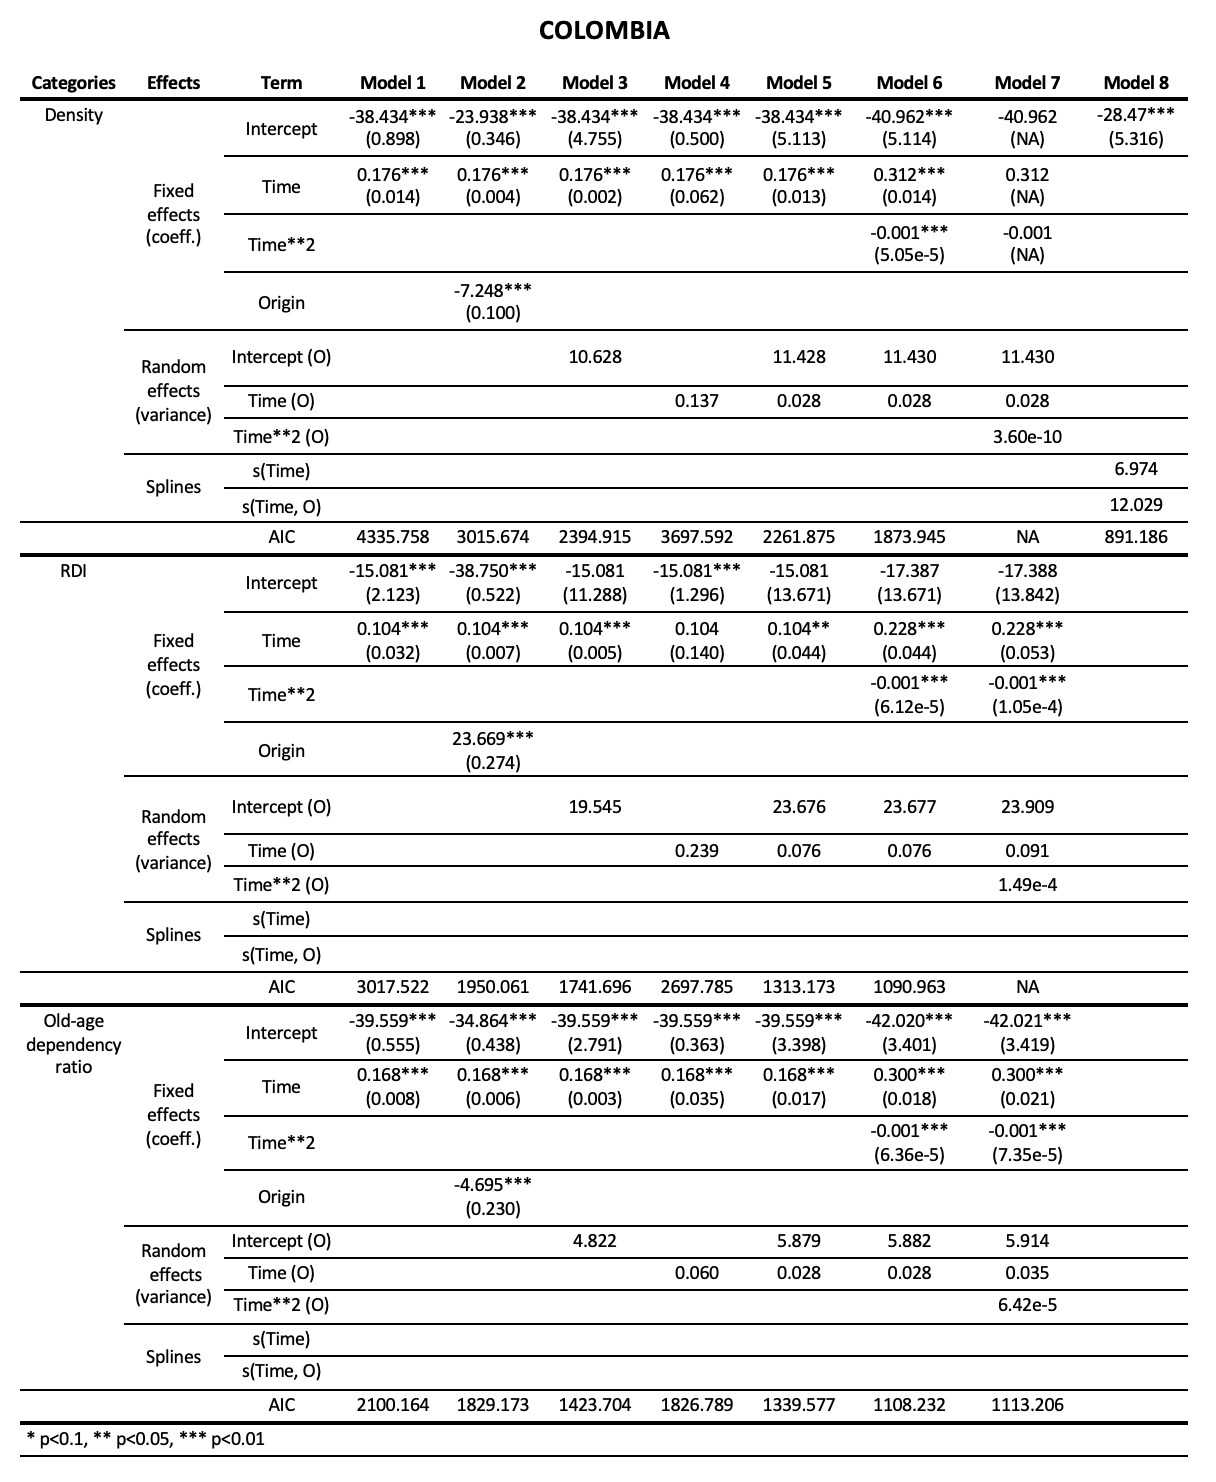
\includegraphics[width=0.9\linewidth]{supplementary/models-tables/models-table-COL-quadratic-new-censored10.png}
\caption{Results of mixed-effects and Generalised Additive Model (GAM) models for trend analysis of relative change in outflows in Colombia. Fixed and random effects according to the population density, the Relative Deprivation Index (RDI) or the old-age dependency ratio of the origin location of outflows are reported for Models 1-7. Effective degrees of freedom are reported for the Spline terms in Model 8.}
\label{tab-modelsCOL}
\end{table}

\clearpage

\begin{table}[h!]
\centering
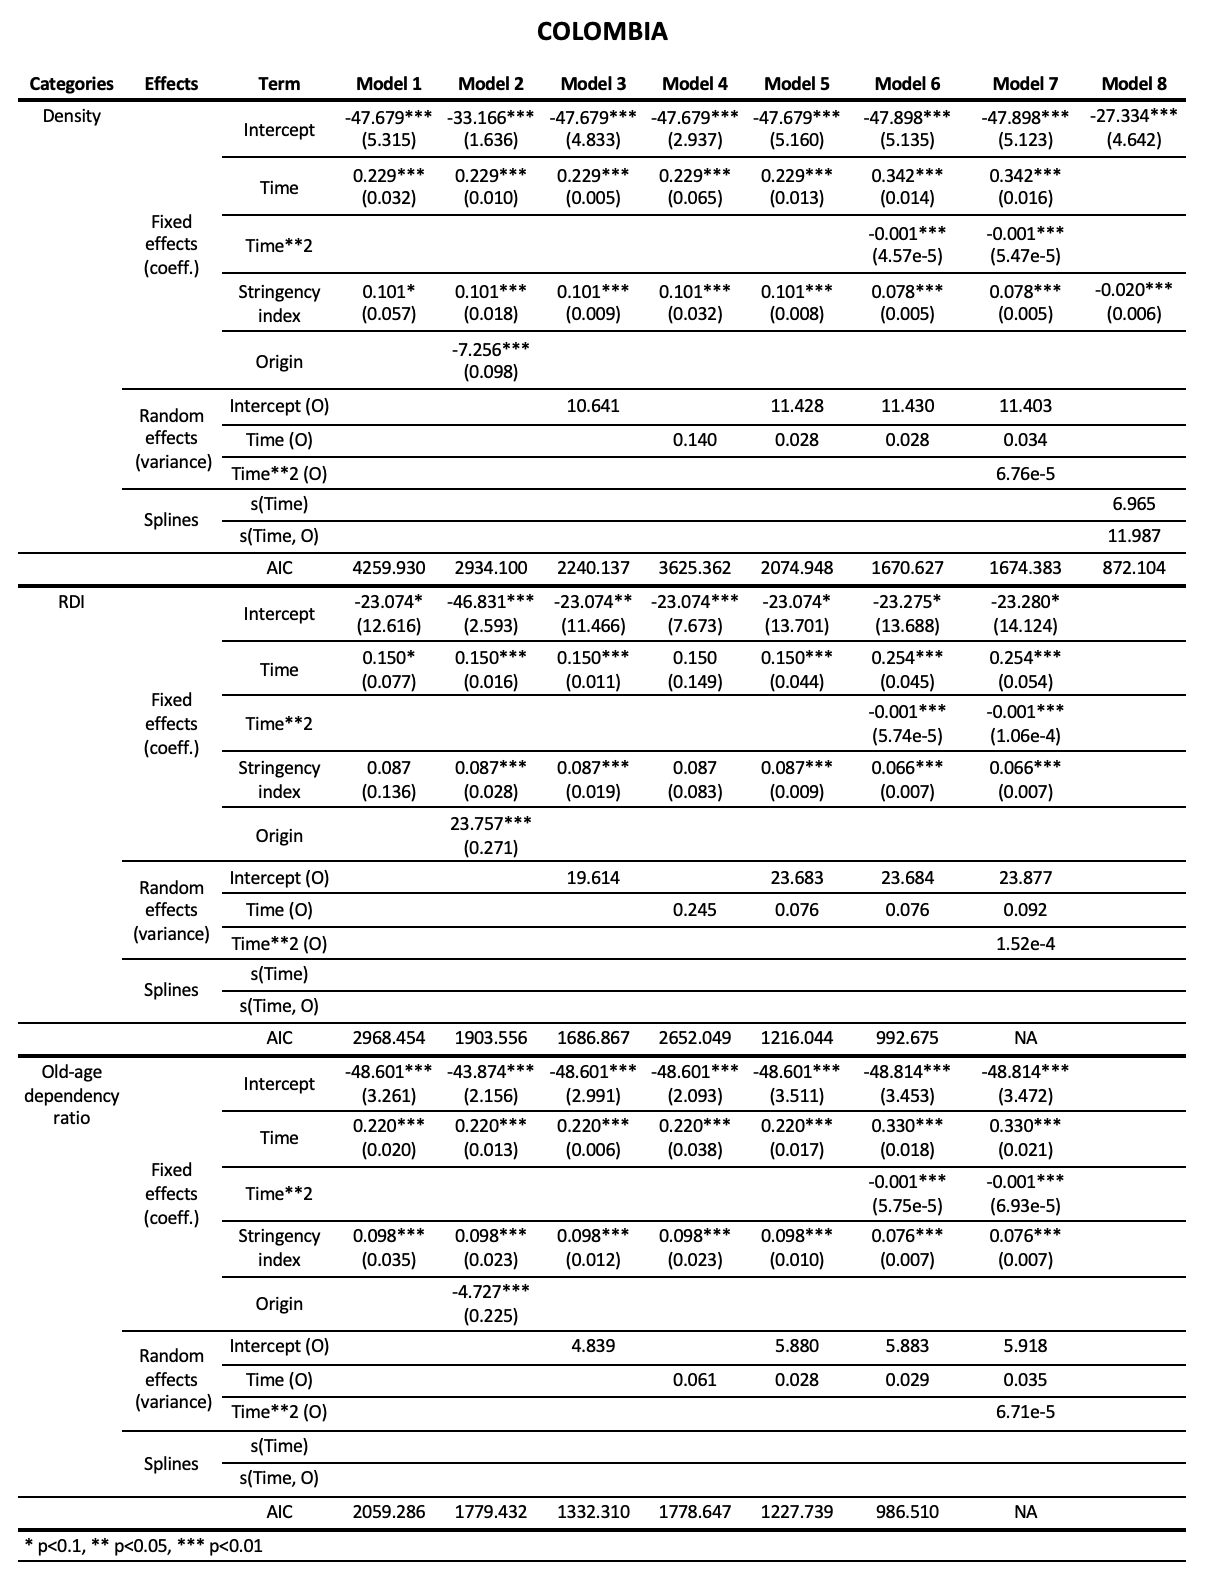
\includegraphics[width=0.9\linewidth]{supplementary/models-tables/models-table-COL-quadratic-stringency-new-censored10.png}
\caption{Results of mixed-effects and Generalised Additive Model (GAM) models for trend analysis of relative change in outflows in Colombia including stringency index as a predictor variable. Fixed and random effects according to the population density, the Relative Deprivation Index (RDI) or the old-age dependency ratio of the origin location of outflows are reported for Models 1-7. Effective degrees of freedom are reported for the Spline terms in Model 8.}
\label{tab-modelsCOL-stringency}
\end{table}

\clearpage

\subsection{Model estimates - relative change in netflows involving capital}

\begin{table}[h!]
\centering
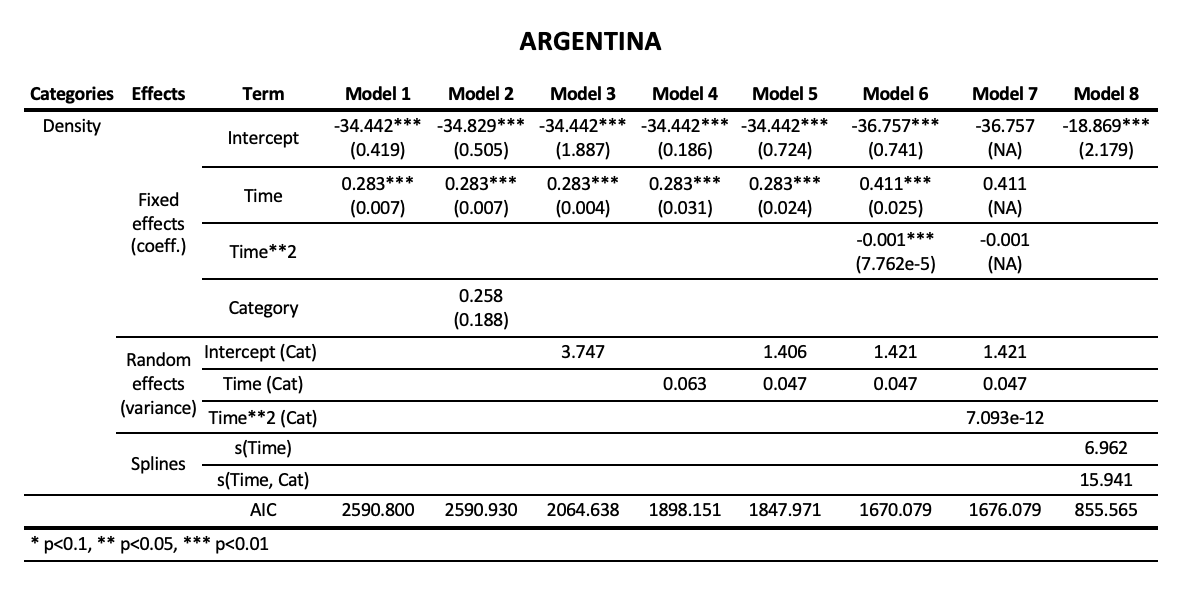
\includegraphics[width=\linewidth]{supplementary/models-tables/models-table-ARG-quadratic-capital-r2.png}
\caption{Results of mixed-effects and Generalised Additive Model (GAM) models for trend analysis of relative change in netflows involving urban region surrounding capital in Argentina. Netflows are defined as inflows to an urban core minus outflows from the urban core. Random effects and spline terms according to population density.}
\label{tab-modelsARG-capital}
\end{table}


\begin{table}[h!]
\centering
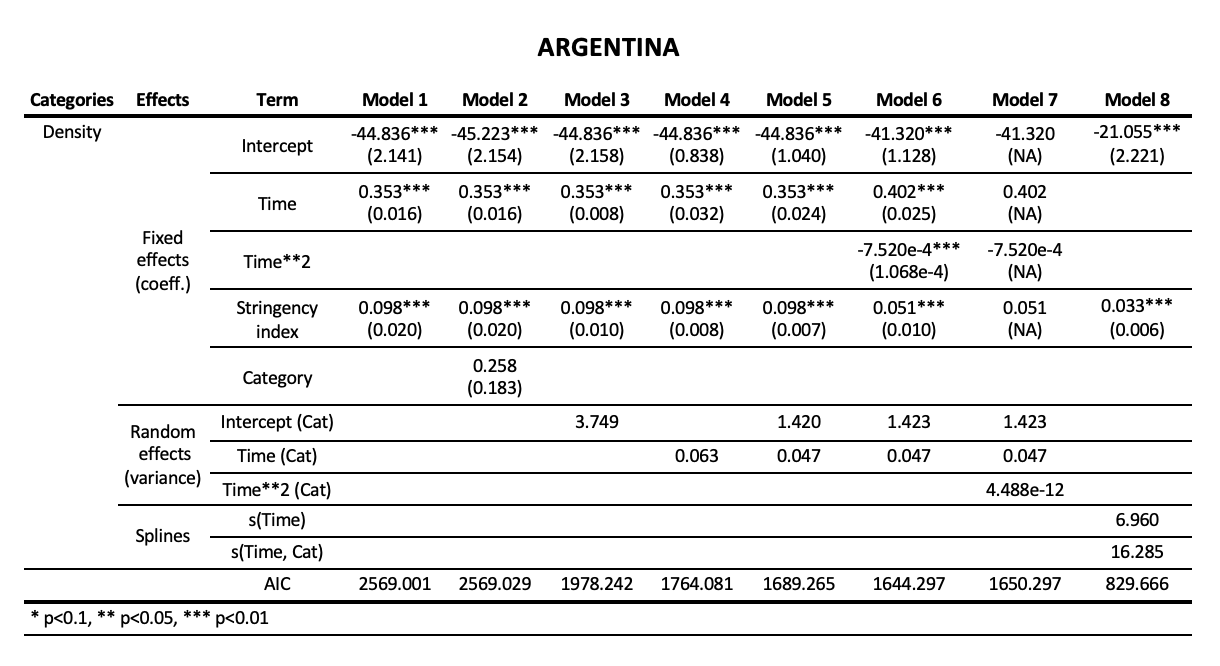
\includegraphics[width=\linewidth]{supplementary/models-tables/models-table-ARG-quadratic-capital-stringency-r2.png}
\caption{Results of mixed-effects and Generalised Additive Model (GAM) models for trend analysis of relative change in netflows involving urban region surrounding capital in Argentina including stringency index as a predictor variable. Netflows are defined as inflows to an urban core minus outflows from the urban core. Random effects and spline terms according to population density.}
\label{tab-modelsARG-capital-stringency}
\end{table}

\newpage

\begin{table}[h!]
\centering
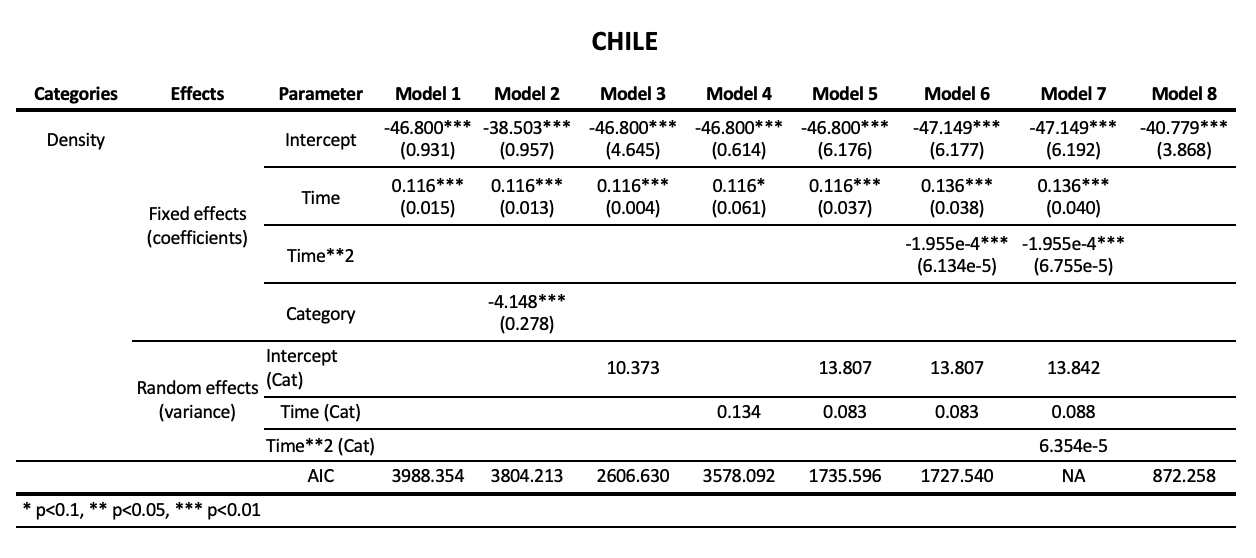
\includegraphics[width=\linewidth]{supplementary/models-tables/models-table-CHL-quadratic-capital-r2.png}
\caption{Results of mixed-effects and Generalised Additive Model (GAM) models for trend analysis of relative change in netflows involving urban region surrounding capital in Chile. Netflows are defined as inflows to an urban core minus outflows from the urban core. Random effects and spline terms according to population density.}
\label{tab-modelsCHL-capital}
\end{table}


\begin{table}[h!]
\centering
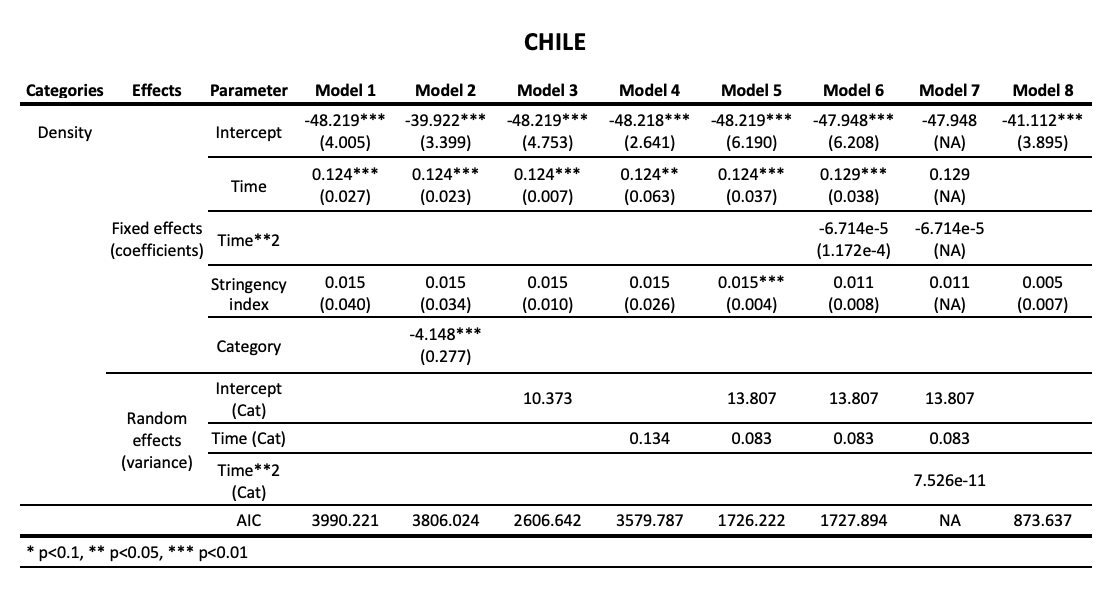
\includegraphics[width=\linewidth]{supplementary/models-tables/models-table-CHL-quadratic-capital-stringency-r2.png}
\caption{Results of mixed-effects and Generalised Additive Model (GAM) models for trend analysis of relative change in netflows involving urban region surrounding capital in Chile including stringency index as a predictor variable. Netflows are defined as inflows to an urban core minus outflows from the urban core. Random effects and spline terms according to population density.}
\label{tab-modelsCHL-capital-stringency}
\end{table}

\newpage

\begin{table}[h!]
\centering
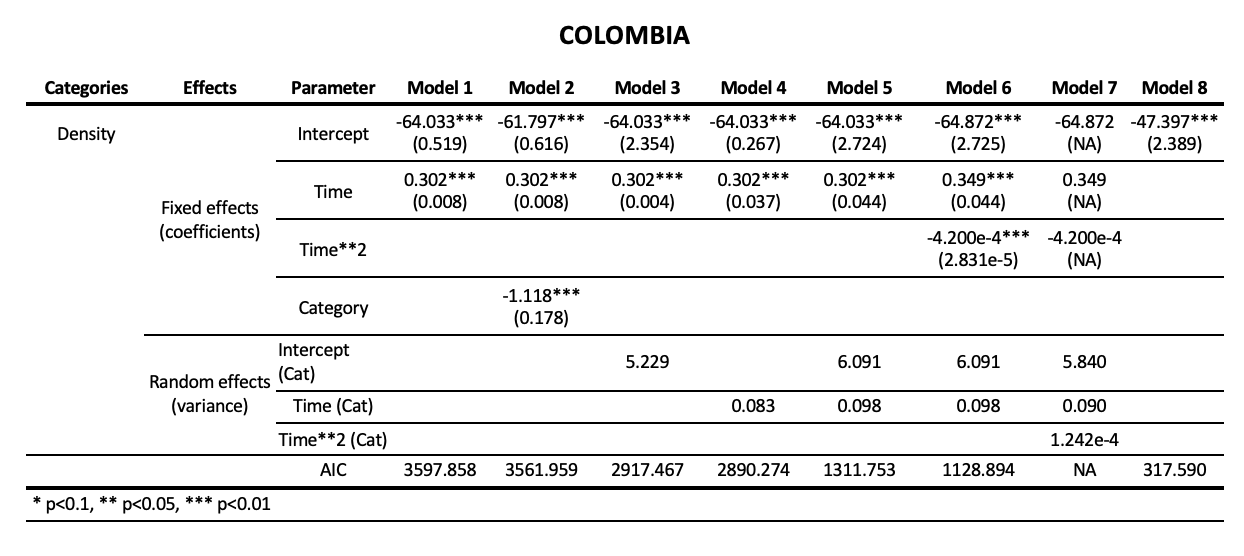
\includegraphics[width=\linewidth]{supplementary/models-tables/models-table-COL-quadratic-capital-r2.png}
\caption{Results of mixed-effects and Generalised Additive Model (GAM) models for trend analysis of relative change in netflows involving urban region surrounding capital in Colombia. Netflows are defined as inflows to an urban core minus outflows from the urban core. Random effects and spline terms according to population density.}
\label{tab-modelsCOL-capital}
\end{table}

\begin{table}[h!]
\centering
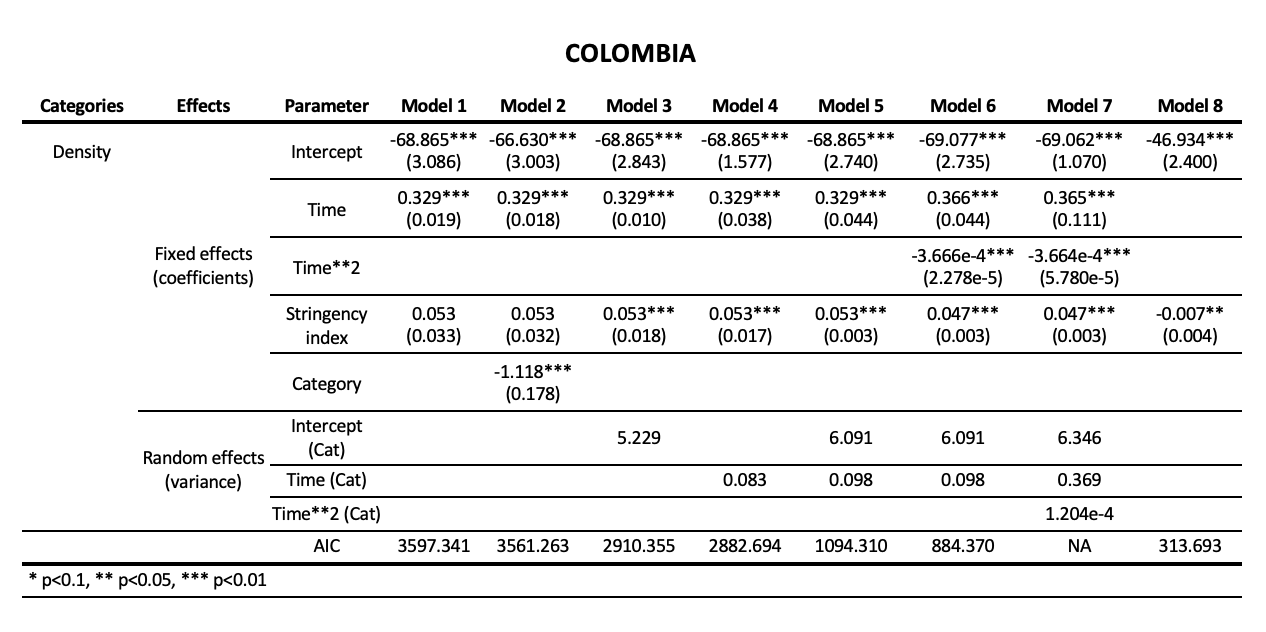
\includegraphics[width=\linewidth]{supplementary/models-tables/models-table-COL-quadratic-capital-stringency-r2.png}
\caption{Results of mixed-effects and Generalised Additive Model (GAM) models for trend analysis of relative change in netflows involving urban region surrounding capital in Colombia including stringency index as a predictor variable. Netflows are defined as inflows to an urban core minus outflows from the urban core. Random effects and spline terms according to population density.}
\label{tab-modelsCOL-capital-stringency}
\end{table}

\clearpage

\subsection{Model estimates - relative change in netflows involving all urban regions}

\begin{table}[h!]
\centering
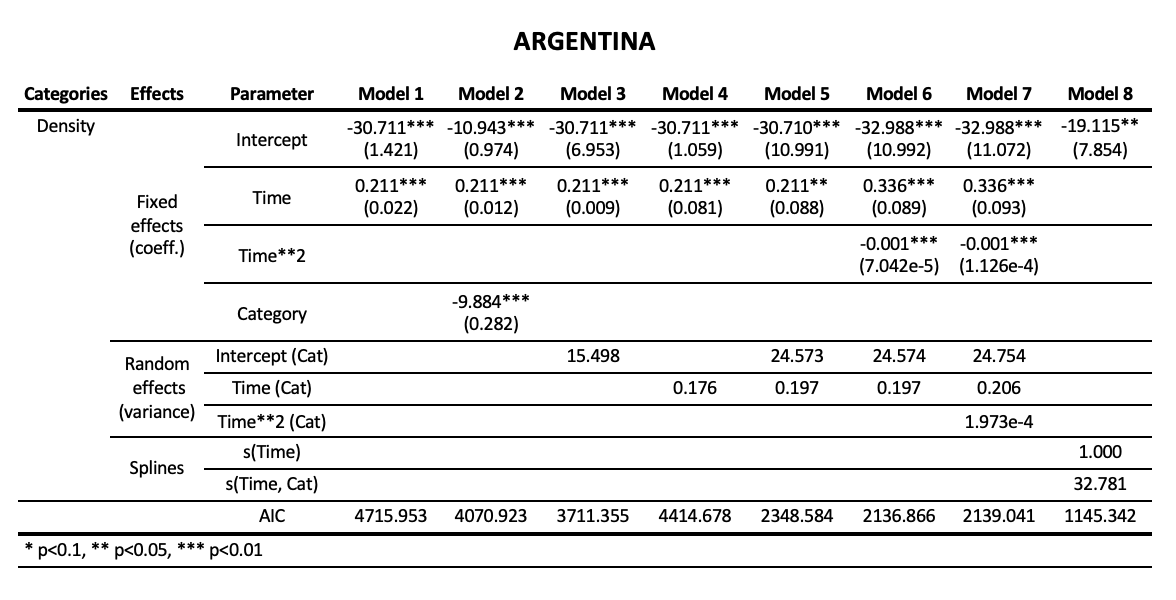
\includegraphics[width=\linewidth]{supplementary/models-tables/models-table-ARG-quadratic-fuas-r2.png}
\caption{Results of mixed-effects and Generalised Additive Model (GAM) models for trend analysis of relative change in netflows involving all urban regions in Argentina. Netflows are defined as inflows to an urban core minus outflows from the urban core. Random effects and spline terms according to population density.}
\label{tab-modelsARG-fuas}
\end{table}

\begin{table}[h!]
\centering
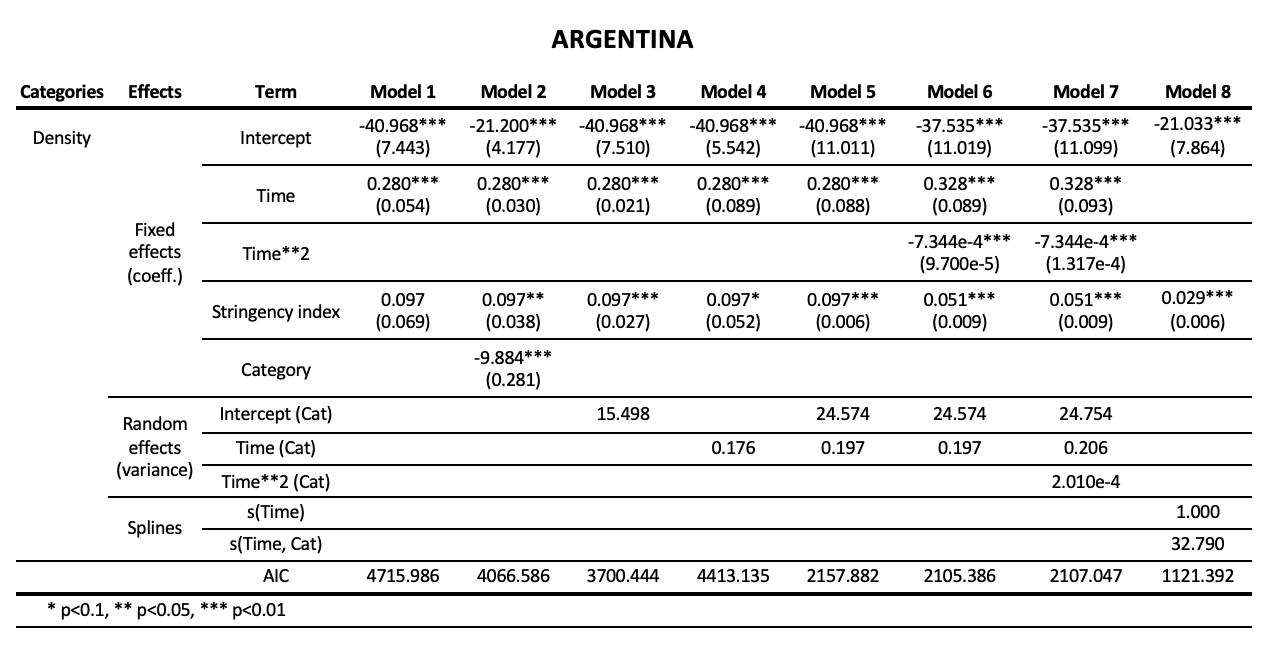
\includegraphics[width=\linewidth]{supplementary/models-tables/models-table-ARG-quadratic-fuas-stringency-r2.png}
\caption{Results of mixed-effects and Generalised Additive Model (GAM) models for trend analysis of relative change in netflows involving all urban regions in Argentina including stringency index as a predictor variable. Netflows are defined as inflows to an urban core minus outflows from the urban core. Random effects and spline terms according to population density.}
\label{tab-modelsARG-fuas-stringency}
\end{table}

\newpage

\begin{table}[h!]
\centering
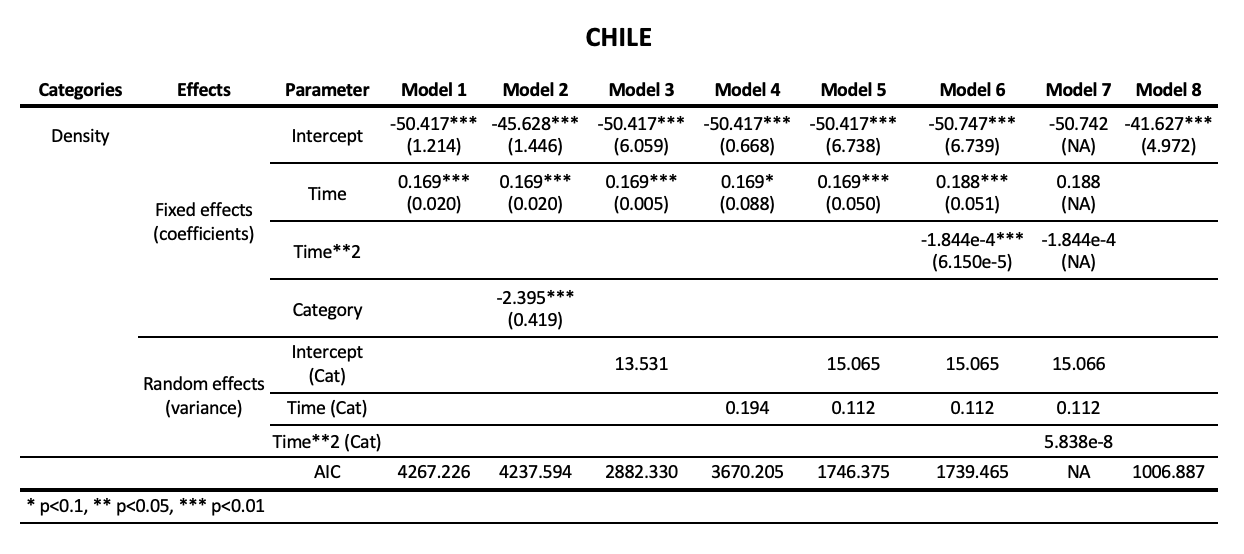
\includegraphics[width=\linewidth]{supplementary/models-tables/models-table-CHL-quadratic-fuas-r2.png}
\caption{Results of mixed-effects and Generalised Additive Model (GAM) models for trend analysis of relative change in netflows involving all urban regions in Chile. Netflows are defined as inflows to an urban core minus outflows from the urban core. Random effects and spline terms according to population density.}
\label{tab-modelsCHL-fuas}
\end{table}

\begin{table}[h!]
\centering
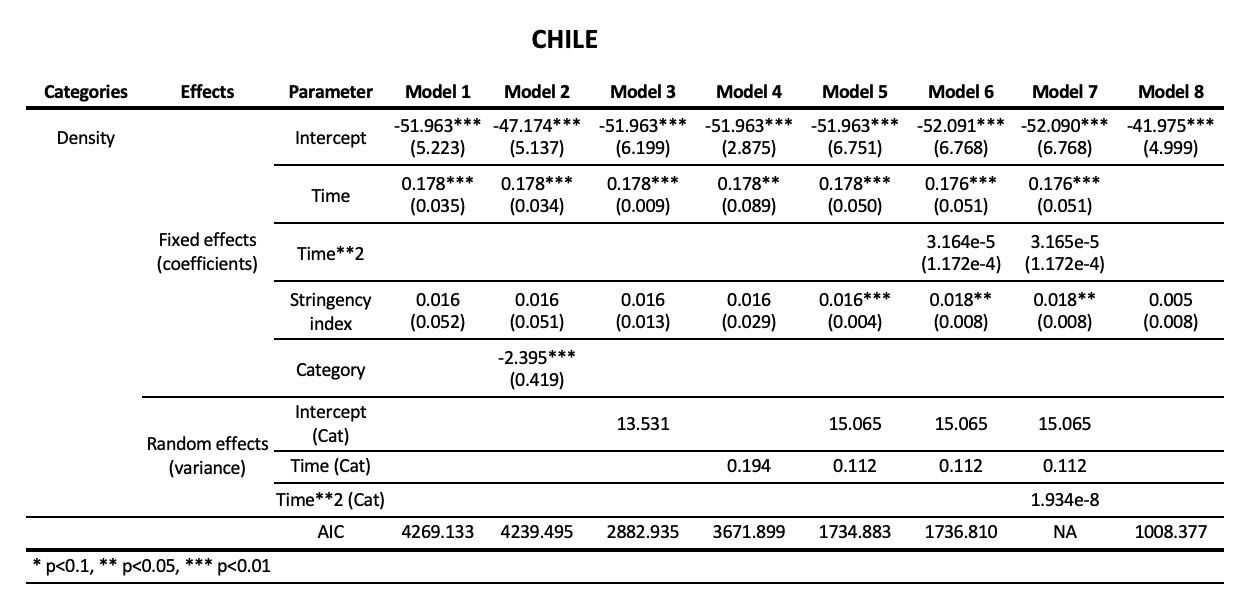
\includegraphics[width=\linewidth]{supplementary/models-tables/models-table-CHL-quadratic-fuas-stringency-r2.png}
\caption{Results of mixed-effects and Generalised Additive Model (GAM) models for trend analysis of relative change in netflows involving all urban regions in Chile including stringency index as a predictor variable. Netflows are defined as inflows to an urban core minus outflows from the urban core. Random effects and spline terms according to population density.}
\label{tab-modelsCHL-fuas-stringency}
\end{table}

\newpage

\begin{table}[h!]
\centering
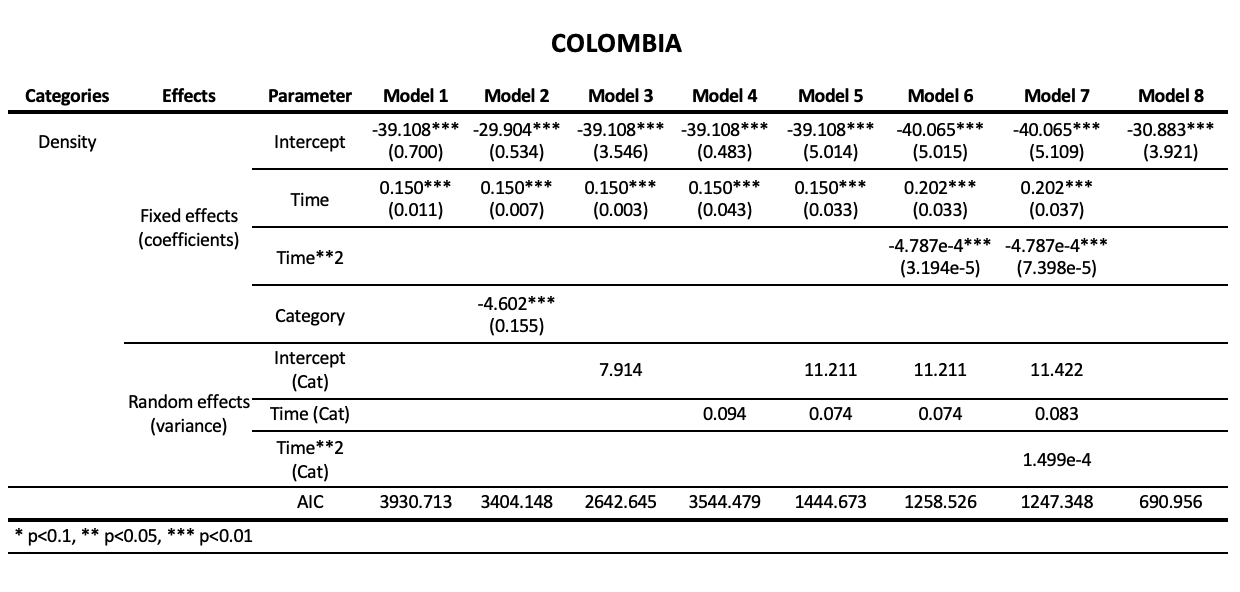
\includegraphics[width=\linewidth]{supplementary/models-tables/models-table-COL-quadratic-fuas-r2.png}
\caption{Results of mixed-effects and Generalised Additive Model (GAM) models for trend analysis of relative change in netflows involving all urban regions in Colombia. Netflows are defined as inflows to an urban core minus outflows from the urban core. Random effects and spline terms according to population density.}
\label{tab-modelsCOL-fuas}
\end{table}

\begin{table}[h!]
\centering
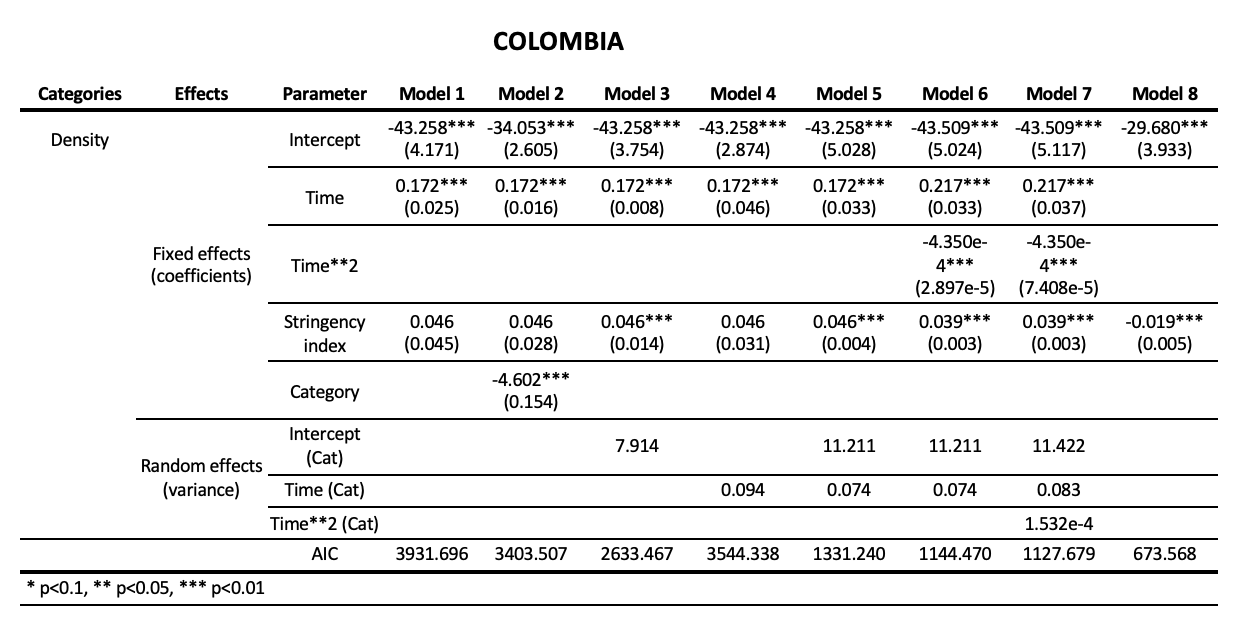
\includegraphics[width=\linewidth]{supplementary/models-tables/models-table-COL-quadratic-fuas-stringency-r2.png}
\caption{Results of mixed-effects and Generalised Additive Model (GAM) models for trend analysis of relative change in netflows involving all urban regions in Colombia including stringency index as a predictor variable. Netflows are defined as inflows to an urban core minus outflows from the urban core. Random effects and spline terms according to population density.}
\label{tab-modelsCOL-fuas-stringency}
\end{table}

\newpage

\subsection{Sensitivity of trend analysis to flow imputation}

\begin{figure}[h!]
\centering
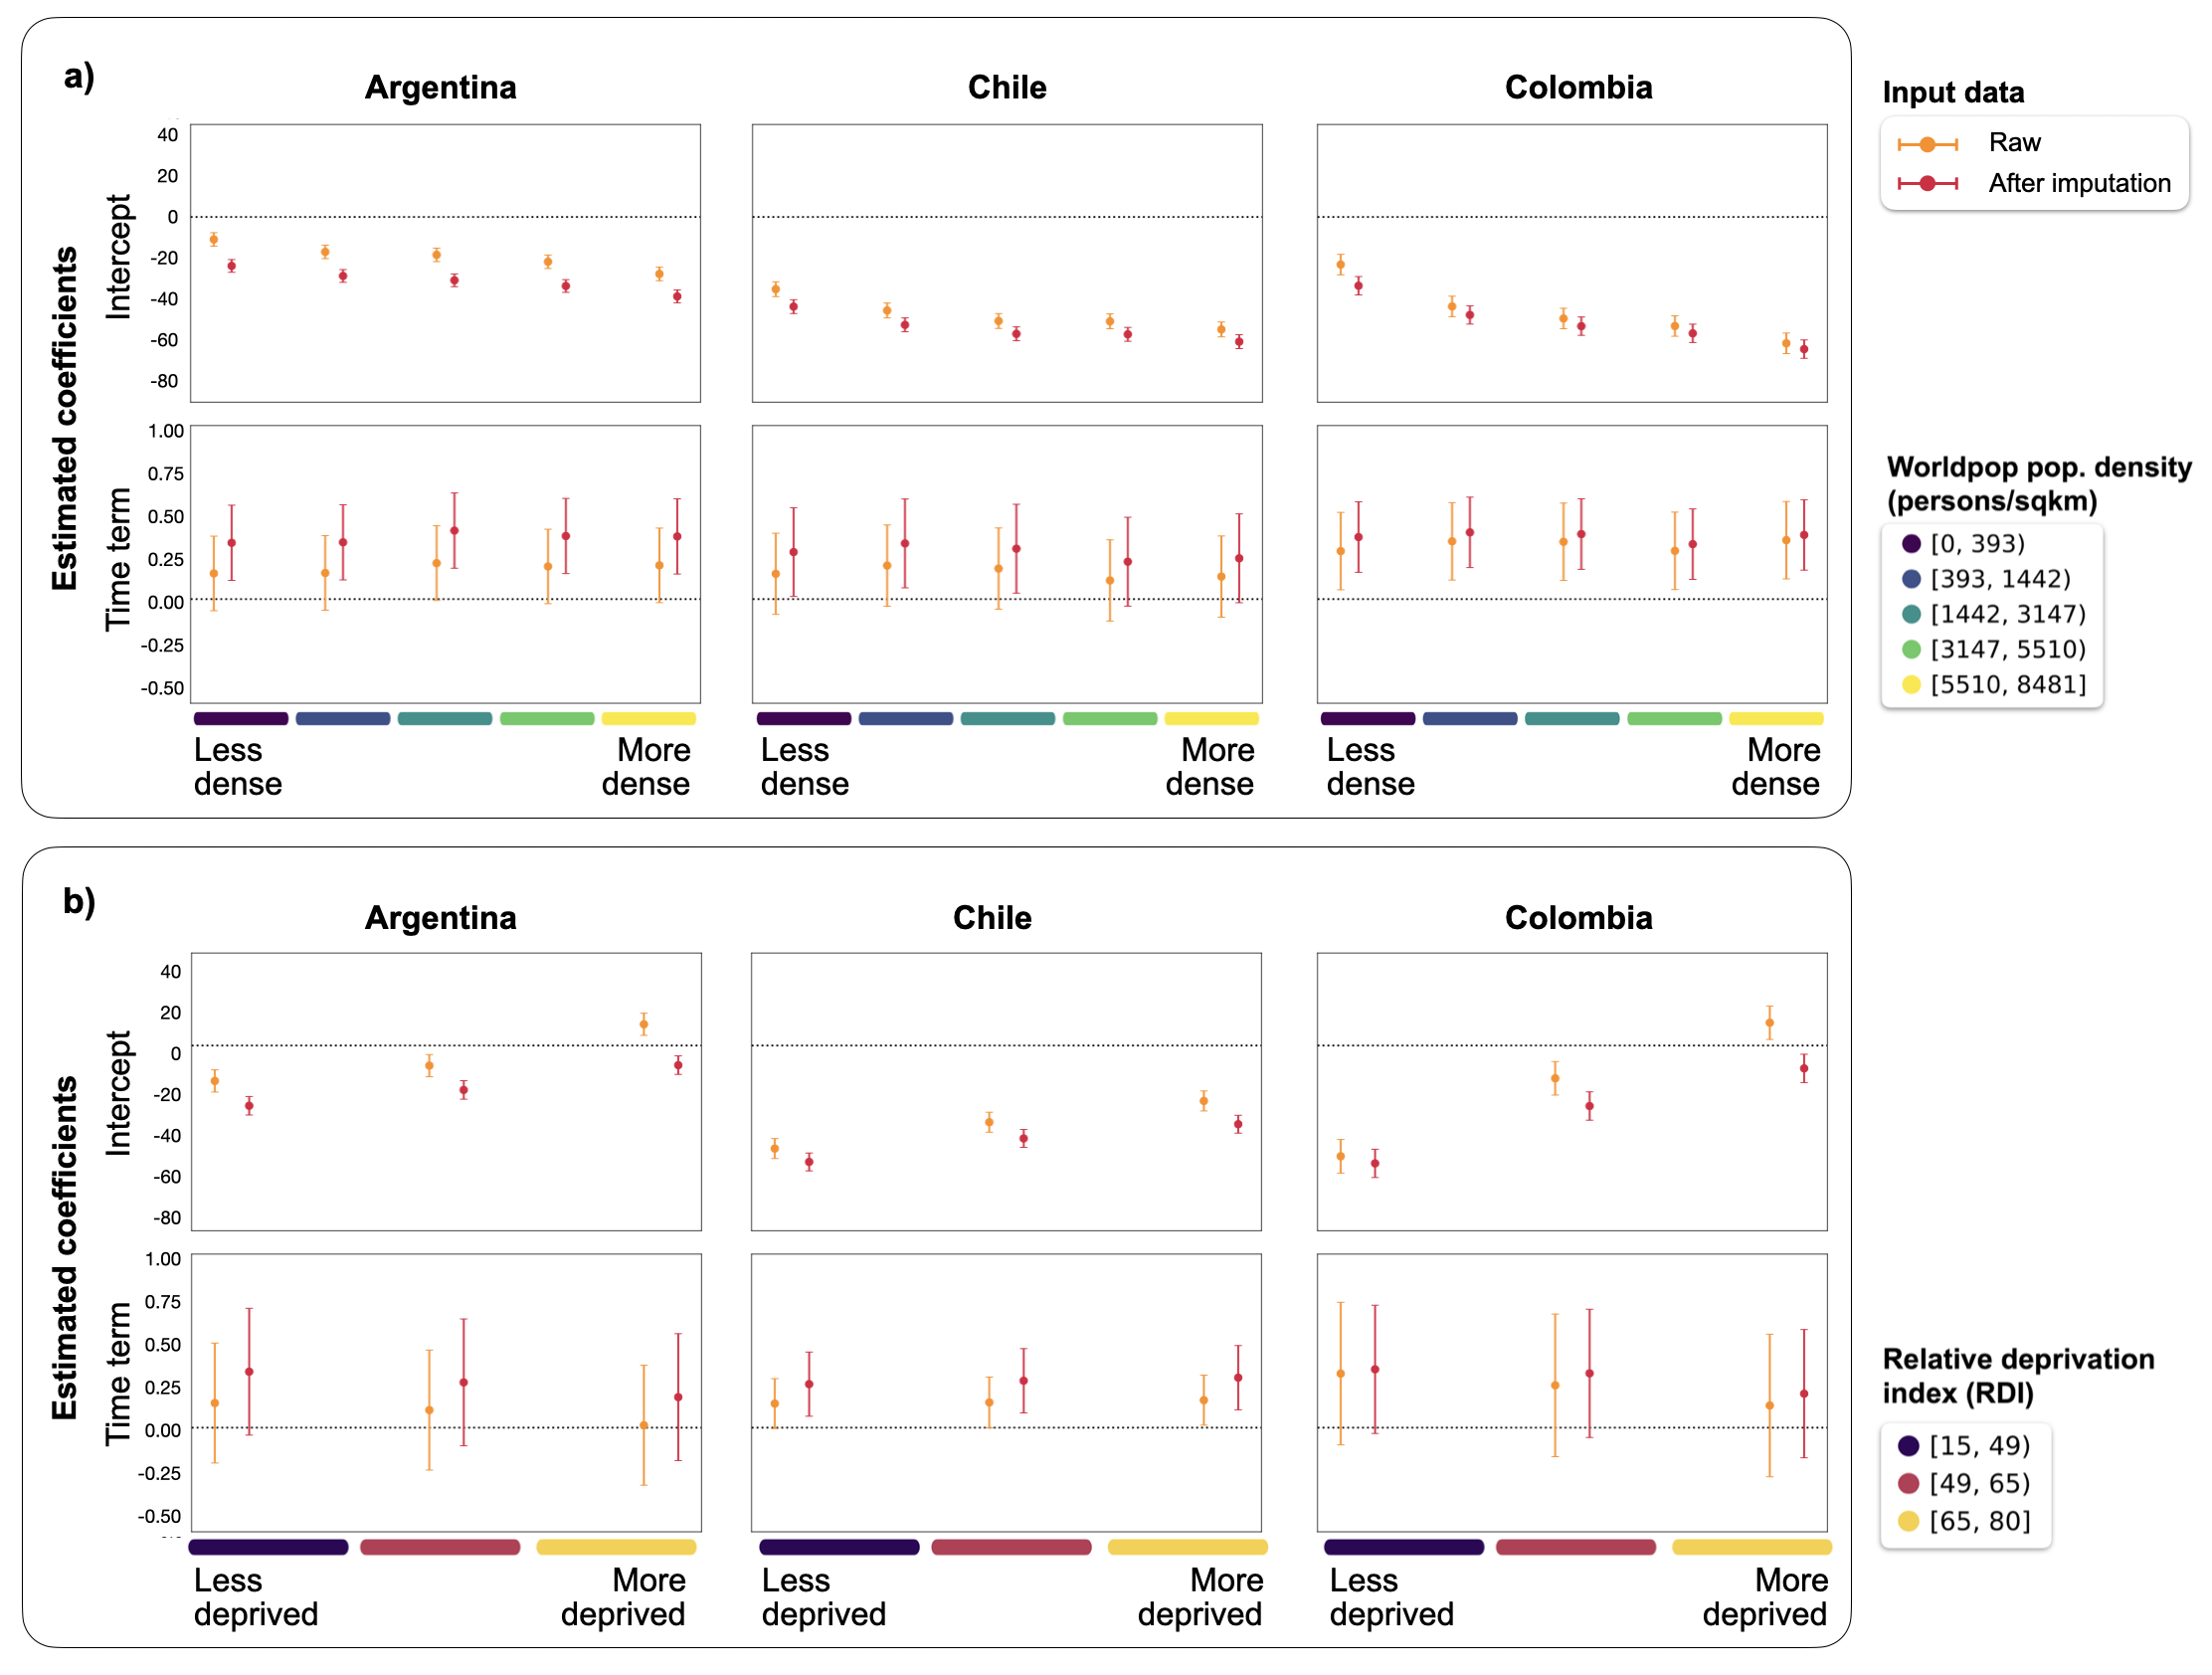
\includegraphics[width=\linewidth]{supplementary/validation-imputation/SF-validation-imputation-models-r2.png}
\caption{Sensitivity of mobility trend estimates to flow imputation across Argentina, Chile and Colombia. Estimated intercept and time coefficients from mixed-effects model 6, fitted to trend series derived from raw data and from imputed data are shown for categories of a) population density and b) relative deprivation index (RDI). Points indicate coefficient estimates and error bars indicate confidence intervals. Colours along the $x$-axis denote the population-density and RDI classes used in each country. Comparing raw and imputed inputs shows how the choice to impute suppressed or missing movement flows can affect the magnitude of the coefficient, but the gradient across density and RDI categories remains consistent.}
\end{figure}

\begin{figure}[h!]
\centering
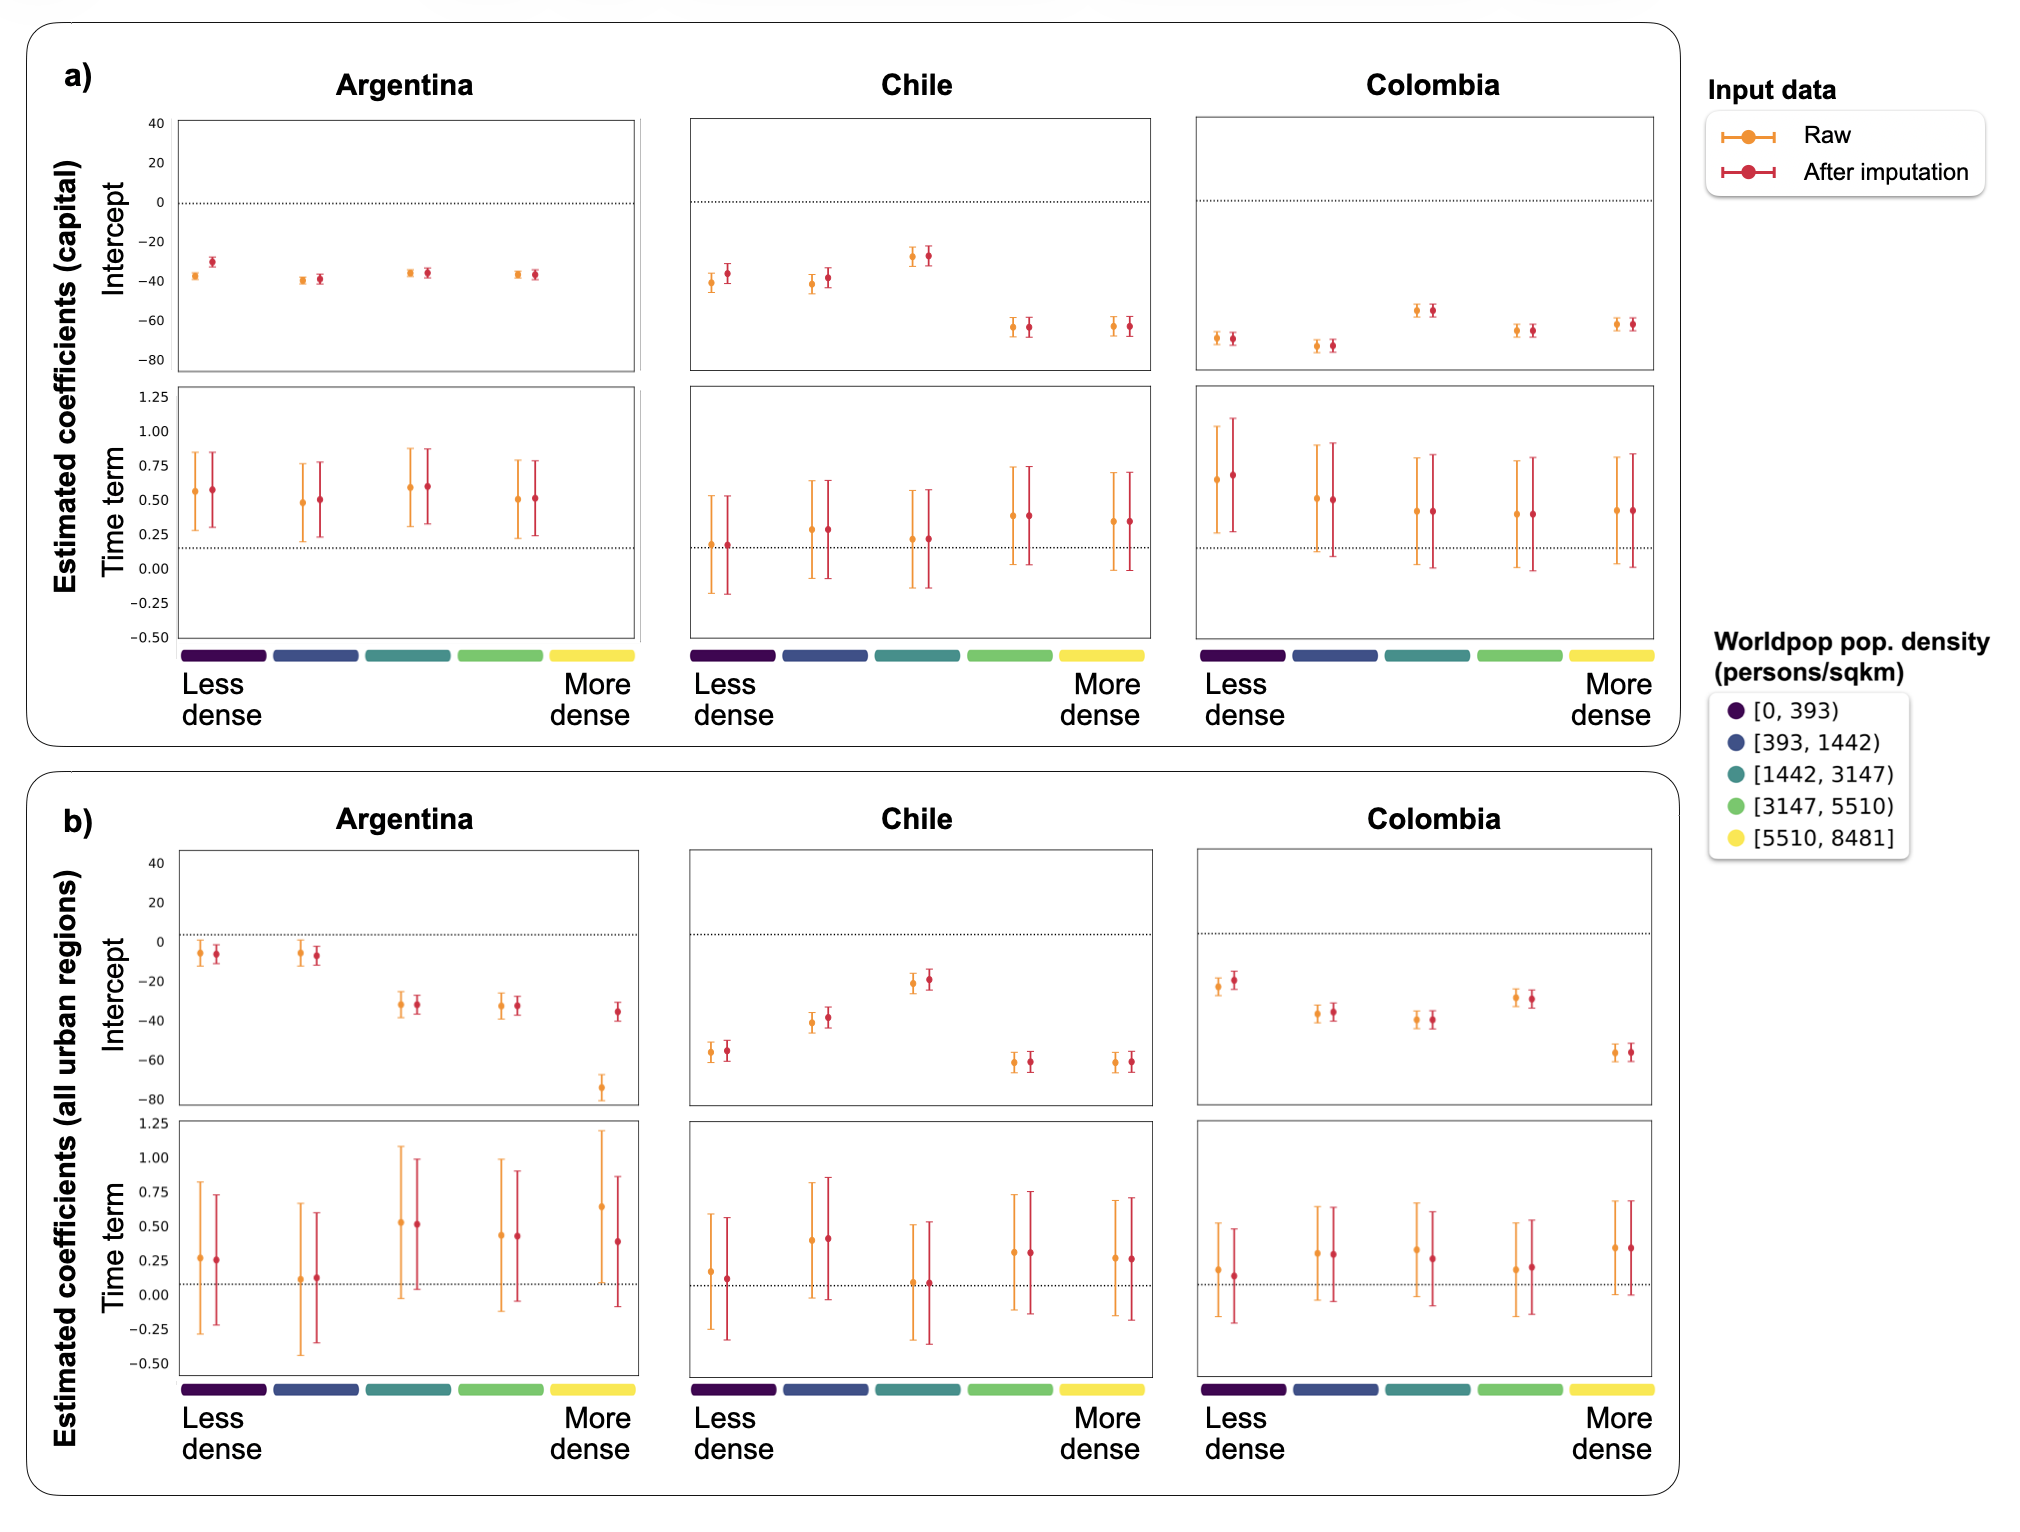
\includegraphics[width=\linewidth]{supplementary/validation-imputation/SF-validation-imputation-models-r2-cities.png}
\caption{Sensitivity of model estimates to flow imputation for mobility trends involving urban cores, across Argentina, Chile and Colombia. Estimated intercept and linear time coefficients from mixed-effects Model 6, fitted to trend series derived from raw and imputed data, are shown for categories of population density for (a) capitals and (b) all functional urban areas (FUAs). Points indicate coefficient estimates and error bars indicate confidence intervals. Colours along the x-axis denote the population-density classes used in each country. Comparing raw and imputed inputs shows that imputing suppressed or missing movement flows can affect coefficient magnitudes, but the gradient across population density categories remains mostly consistent for capitals and FUAs.}
\end{figure}

\newpage

\section{Recovery times}

\subsection{Deriving recovery time formula (equation 7)}

We begin by assuming a quadratic model to describe the evolution of mobility levels over time relative to the baseline:
\begin{equation}
    y(t) = a + b\cdot t + c\cdot t^2
\end{equation}\label{model-trend}

The coefficients \( a \), \( b \), and \( c \) can be expressed in terms of the parameters from equation (6) in the main text. For instance, under Model 6, we have \( a = \beta_0 + b_0 \), \( b = \beta_1 + b_{1i} \), and \( c = \beta_2 \).

The recovery time to a threshold \( \alpha \), denoted by \( t_{\alpha} \), is defined as the time it takes for \( y(t) \) to recover by \( \alpha\% \). If the mobility level relative to the baseline at time \( t = 0 \) is \( a \), then \( t_{\alpha} \) is the time at which
\[
y(t_{\alpha}) = \left(1 - \frac{\alpha}{100}\right) a.
\]

Substituting this into equation \eqref{model-trend} and solving for \( t_{\alpha} \), we obtain:
\begin{equation}
    t_{\alpha} = \frac{-b \pm \sqrt{b^2 - 4c \left( \frac{\alpha}{100} \right) a}}{2c}
\end{equation}\label{recovery-time}

A recovery time is only meaningful if mobility initially decreased relative to the baseline, which imposes the condition \( a < 0 \). Moreover, since we are referring to a ``recovery,'' the trend must be increasing at \( t = 0 \), requiring \( y'(0) > 0 \), or equivalently, \( b > 0 \). As we are only interested in positive time values, and given \( b > 0 \), we select the solution with the \( + \) sign in equation \eqref{recovery-time}.

Finally, if \( b^2 - 4c \left( \frac{\alpha}{100} \right) a < 0 \), there is no real-valued solution for \( t_{\alpha} \). In such cases, we interpret this as mobility levels never reaching the specified recovery threshold.

The recovery time can also be obtained under a linear model (e.g. Model 5). The derivation is then analogous, but $y(t) = a + b\cdot t$ and therefore, $t_\alpha$ is given by:
\begin{equation}
    t_{\alpha} = -\dfrac{\alpha}{100}\cdot \dfrac{a}{b}
\end{equation}

\subsection{Computation of uncertainty for recovery times}

According to Model 6, the recovery time at threshold $\alpha$ is given by equation \eqref{recovery-time} where $a$, $b$ and $c$ are the coefficients for the intercept, linear and quadratic terms in equation \eqref{model-trend}.

The partial derivatives are:
\[
\frac{\partial t_\alpha}{\partial a} = \frac{-\frac{\alpha}{100}}{\sqrt{b^2 - 4c\frac{\alpha}{100} a}}, \quad
\frac{\partial t_\alpha}{\partial b} = \frac{1}{2c} \left( -1 + \frac{b}{\sqrt{b^2 - 4c\frac{\alpha}{100} a}} \right), \quad
\frac{\partial t_\alpha}{\partial c} = \frac{(b - \sqrt{b^2 - 4c\frac{\alpha}{100} a})\sqrt{b^2 - 4c\frac{\alpha}{100} a} - 2\frac{\alpha}{100} a c}{2c^2\sqrt{b^2 - 4c\frac{\alpha}{100} a}}
\]

The propagated uncertainty is:
\[
\sigma_t = \sqrt{
\left( \frac{\partial t_\alpha}{\partial a} \right)^2 \sigma_a^2 +
\left( \frac{\partial t_\alpha}{\partial b} \right)^2 \sigma_b^2 +
\left( \frac{\partial t_\alpha}{\partial c} \right)^2 \sigma_c^2}
\]

If using a linear model to estimate $t_{\alpha}$, like Model 5, then:
\[
\frac{\partial t_\alpha}{\partial a} = -\frac{\alpha}{100} \cdot \frac{1}{b}, \quad
\frac{\partial t_\alpha}{\partial b} = \dfrac{\alpha}{100}\cdot\dfrac{a}{b^2}
\]
and the propagated uncertainty is 
\begin{displaymath}
    \sigma_{t_\alpha} = \sqrt{
\left( \frac{\partial t_\alpha}{\partial a} \right)^2 \sigma_a^2 +
\left( \frac{\partial t_\alpha}{\partial b} \right)^2 \sigma_b^2 }
\end{displaymath}

\newpage

\subsection{Estimated recovery times}

\begin{table}[h!]
\centering
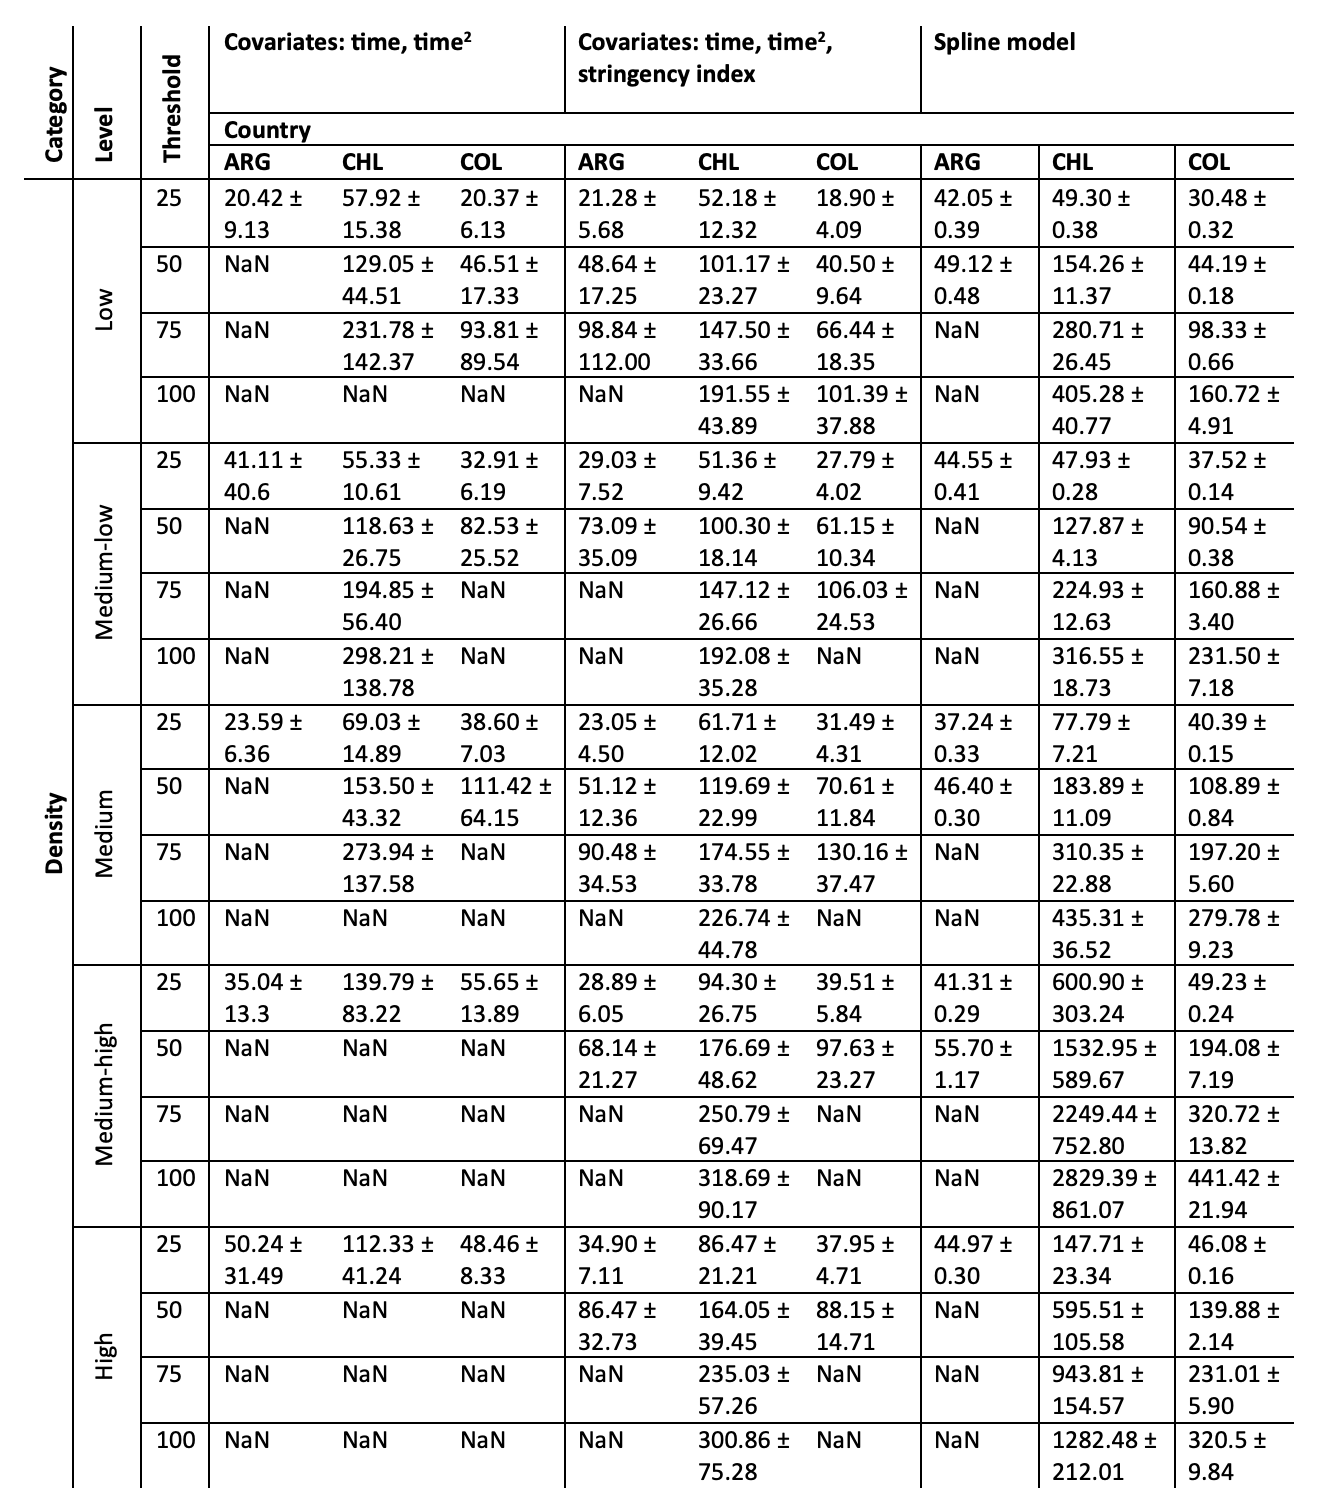
\includegraphics[width=0.9\linewidth]{supplementary/recovery-times/recovery-thresholds-table-quadratic-std-density-censored10.png}
\caption{Recovery times at multiple thresholds, for outflows in Argentina, Chile and Colombia, by population density. Computed using Model 6 (with covariates time and time$^2$, or time, time$^2$ and stringency index) or according to the GAM model (Model 8). N/A values correspond to cases where the initial mobility levels are above the baseline. NaN values correspond to cases where mobility never recovers to the specified threshold.}
\end{table}


\newpage 


\begin{table}[h!]
\centering
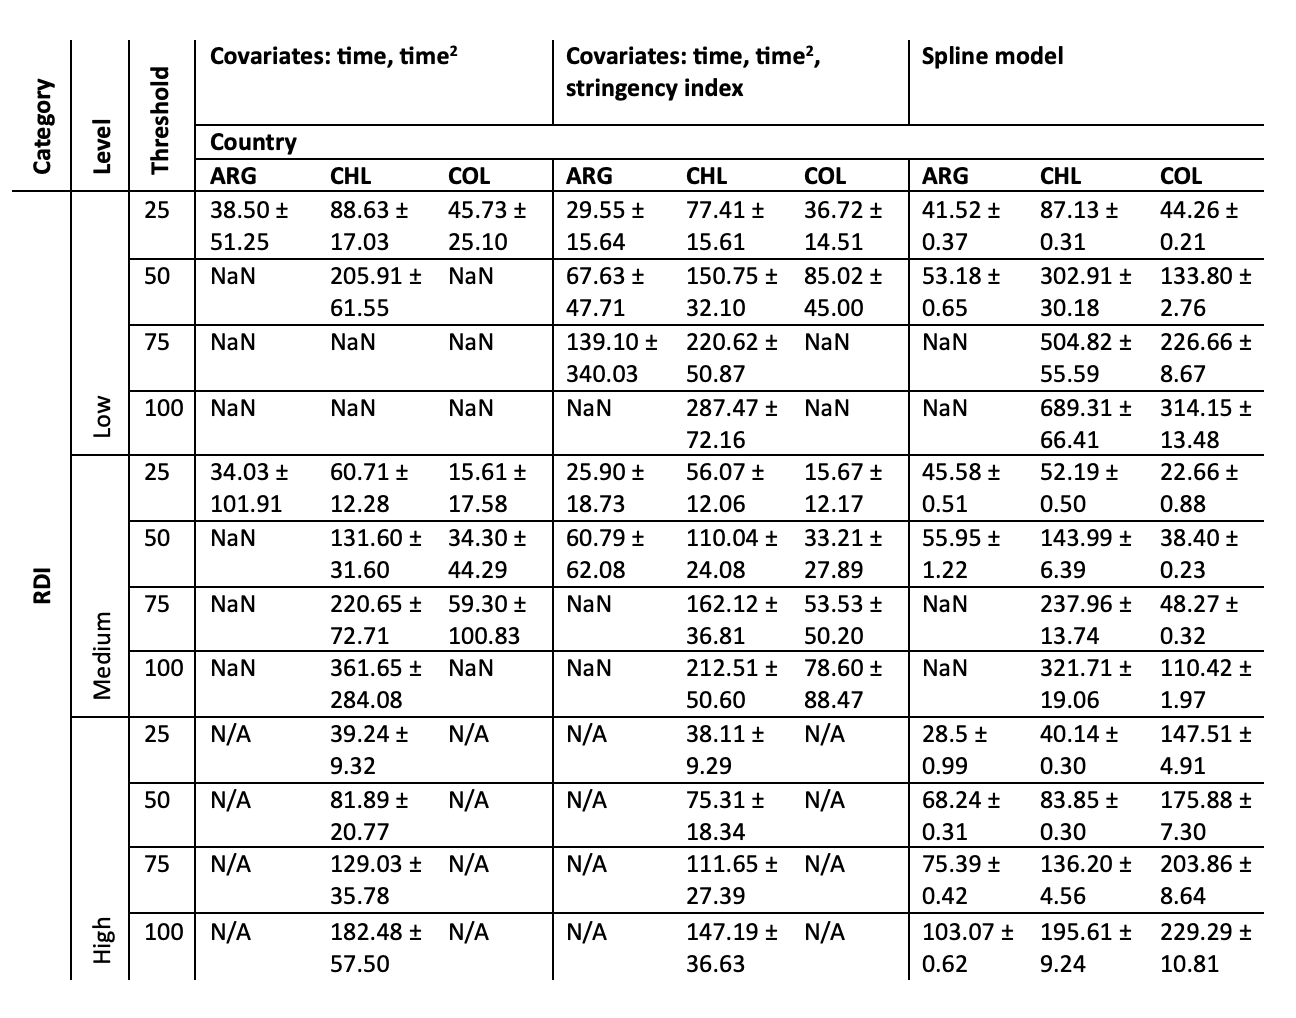
\includegraphics[width=0.9\linewidth]{supplementary/recovery-times/recovery-thresholds-table-quadratic-std-rdi-censored10.png}
\caption{Recovery times at multiple thresholds, for outflows in Argentina, Chile and Colombia, by Relative Deprivation Index (RDI) category. Computed using Model 6 (with covariates time and time$^2$, or time, time$^2$ and stringency index) or according to the GAM model (Model 8). N/A values correspond to cases where the initial mobility levels are above the baseline. NaN values correspond to cases where mobility never recovers to the specified threshold.}
\end{table}

\newpage

\begin{table}[h!]
\centering
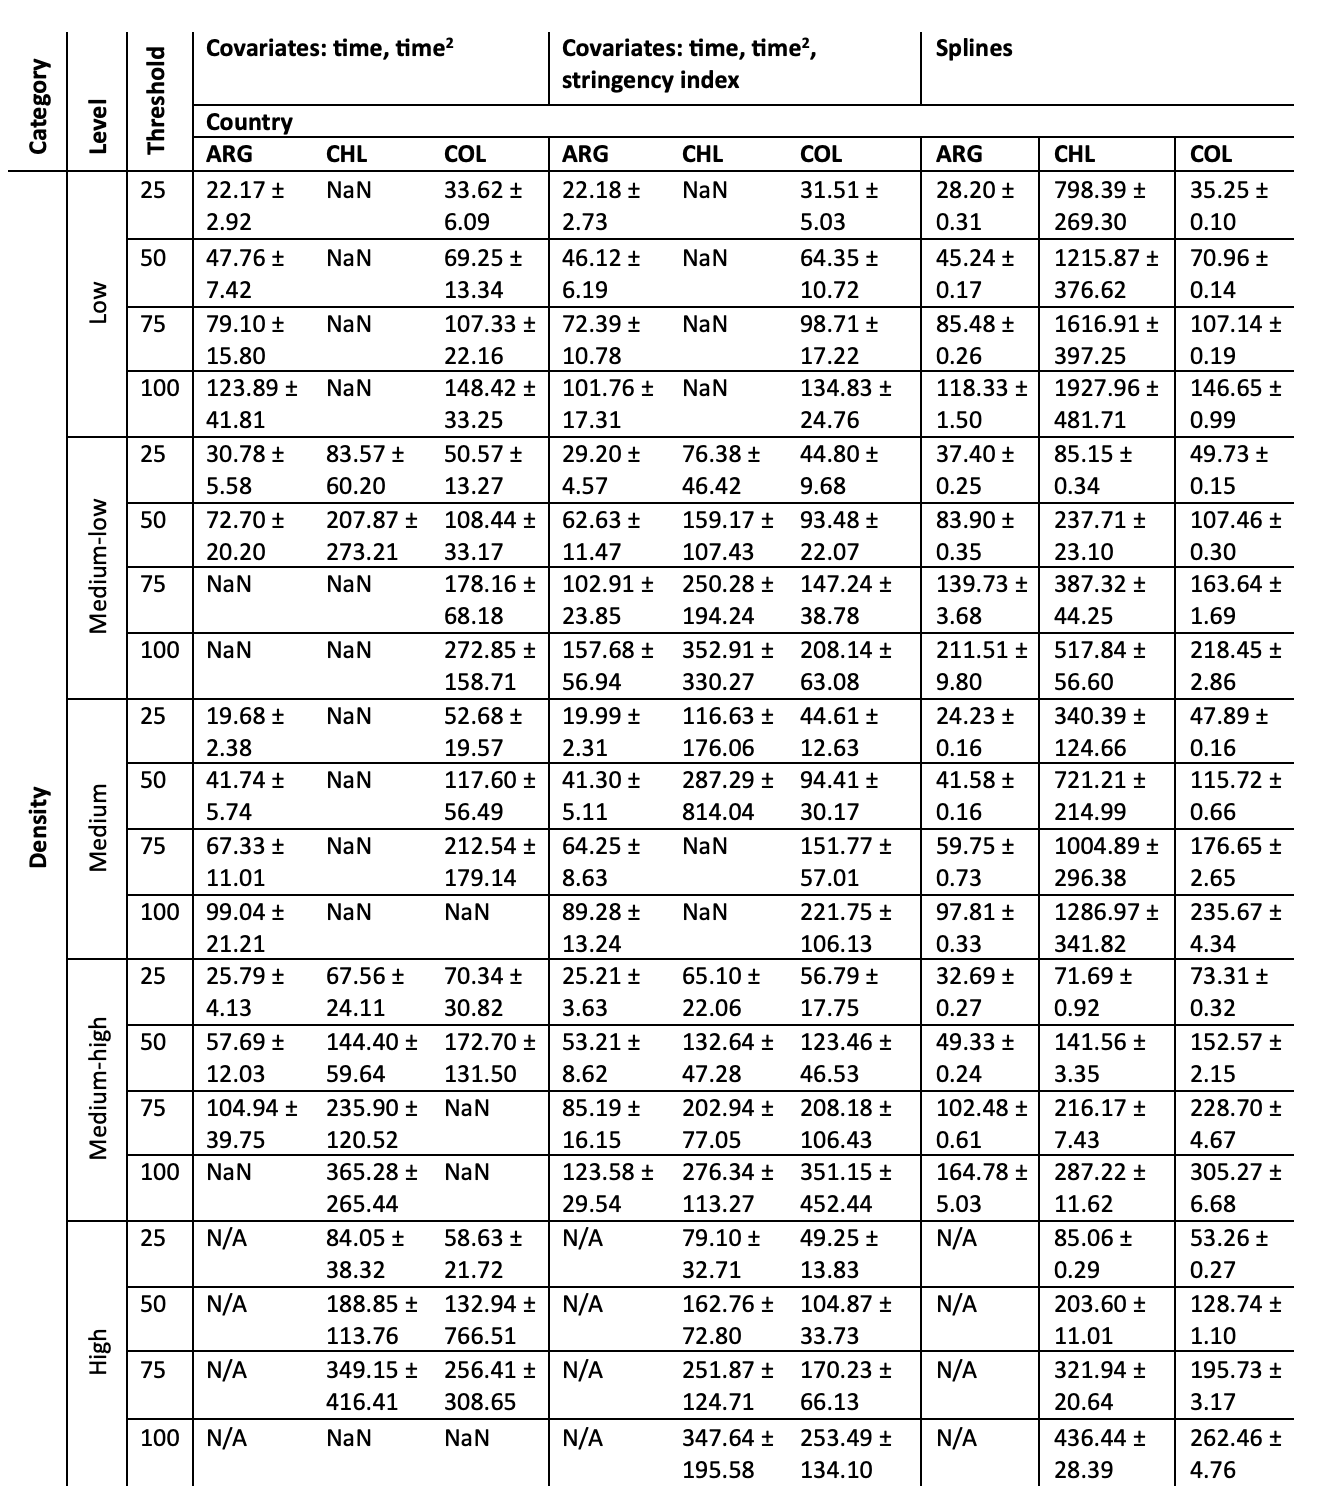
\includegraphics[width=0.9\linewidth]{supplementary/recovery-times/recovery-thresholds-table-quadratic-capital-std-r2.png}
\caption{Recovery times at multiple thresholds, for netflows involving the urban region surrounding the capital in Argentina, Chile and Colombia, by population density category. Computed using Model 6 (with covariates time and time$^2$, or time, time$^2$ and stringency index) or according to the GAM model (Model 8). N/A values correspond to cases where the initial mobility levels are above the baseline or the only cell in a population density category is the centre of netflows. NaN values correspond to cases where mobility never recovers to the specified threshold.}
\label{tab-rec-times-capital}
\end{table}

\newpage

\begin{table}[h!]
\centering
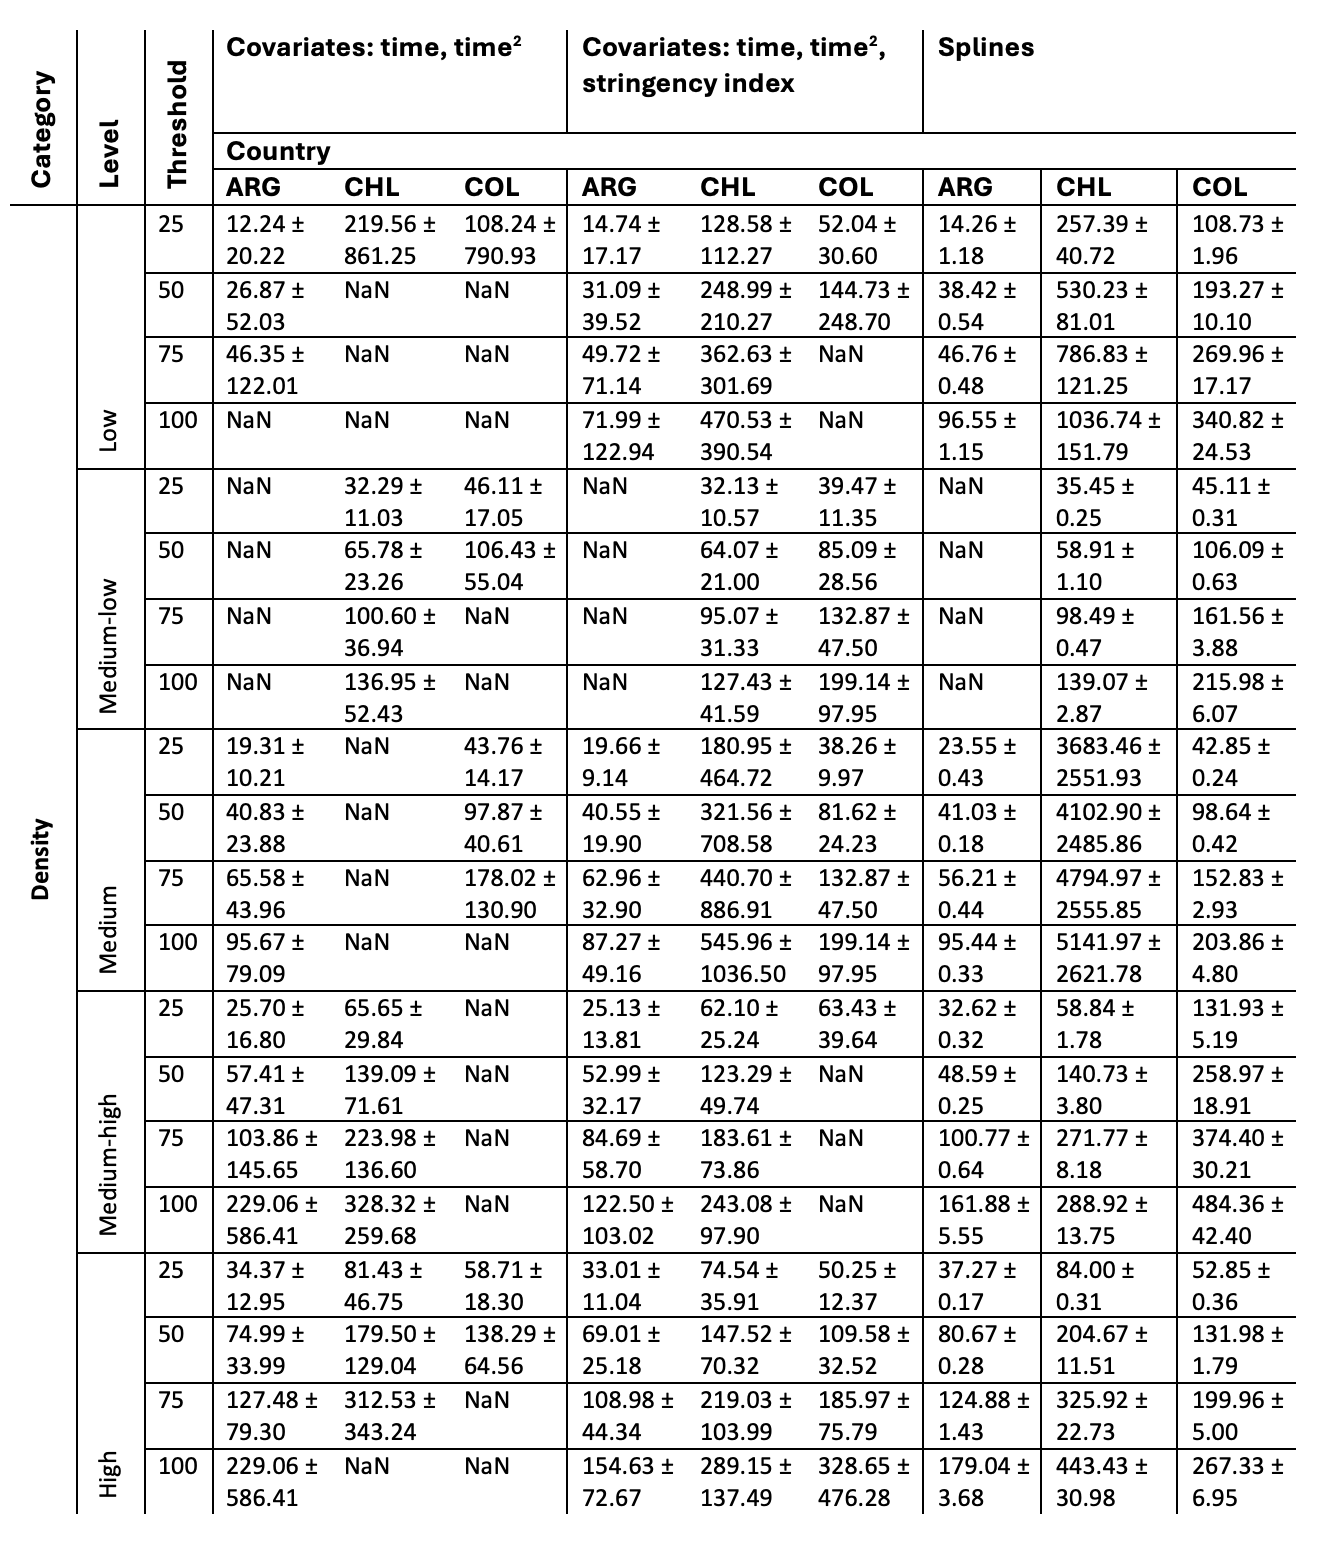
\includegraphics[width=0.9\linewidth]{supplementary/recovery-times/recovery-thresholds-table-quadratic-fuas-std-r2.png}
\caption{Recovery times at multiple thresholds, for netflows involving all urban regions in Argentina, Chile and Colombia, by population density category. Computed using Model 6 (with covariates time and time$^2$, or time, time$^2$ and stringency index) or according to the GAM model (Model 8). NaN values correspond to cases where mobility never recovers to the specified threshold.}
\label{tab-rec-times-fuas}
\end{table}

\newpage


\section{Supplementary Note 1: External consistency checks for mobility recovery patterns}


To externally validate the results from our analysis, we reviewed independent official statistics and survey evidence from settings covered by the study and from the wider Latin American and Caribbean region. These sources do not enable validation at the spatial and temporal resolution of our analysis, but they offer useful external consistency checks on the broad dynamics that we also identified.

For Argentina, we consulted the official Buenos Aires mobility monitoring reports produced by the ``Observatorio de Movilidad y Seguridad Vial'' \cite{OMSV2026BA}. These reports show a sharp decline in mobility during the pandemic period followed by gradual but incomplete recovery. By March 2026, daily unique public transport users in Buenos Aires remained 19.7\% below the same month in 2019, suggesting that urban mobility had not fully returned to its pre-pandemic baseline.

For Chile, we reviewed the 2024 Santiago Mobility Survey (EMS) \cite{Hurtubia2024EMS}. Its results are not directly comparable to our analysis because they focus on the relative use of different transport modes rather than longitudinal recovery in aggregate mobility levels. Yet, the report explicitly notes the value of complementary sources to better understand patterns of mobility, including mobile-phone and other digital trace data such as Meta's, when conventional surveys are infrequent or limited in scope.

For Colombia, we consulted the ``Encuesta de Transporte Urbano de Pasajeros'' (ETUP) produced by the National Administrative Department of Statistics (DANE), which covers 8 metropolitan areas and 15 cities \cite{DANE2025}. The data shows a decline in public transport demand in 2020 followed by incomplete recovery over time. Total passengers transported fell from 934.978 million in the fourth quarter of 2019 to 534 million in 2020, and then recovered to 682 million in 2021, 757 million in 2022, 776 million in 2023, 789 million in 2024 and 754 million in 2025. This evolution is consistent with the broad recovery dynamics identified in our analysis.

We also reviewed recent evidence for Latin America and the Caribbean, produced by the UN International Labour Organization (ILO) \cite{ILO2023PanoramaLaboral, BertranouGontero2024LACWork}. The ILO reports show that, before the pandemic, only around 3\% of employed people in the region worked remotely, whereas this proportion rose to 20--30\% during COVID-19 while lockdown measures were in place. Although remote work declined afterwards, it remained above pre-pandemic levels. For example, in Chile, the proportion of home workers increased from 4.6\% of all workers in 2019 to 21\% in 2020, before falling to 8.6\% in 2023. However, in absolute terms, the number of people working from home in 2023 remained 86\% higher than in 2019. These figures, based on national labour and household surveys, provide further external evidence consistent with our finding that daily mobility volumes have not fully returned to their pre-COVID baseline and are likely driven by higher engagement with remote work.


\bibliography{bibliography}

\end{document}